\documentclass[11pt,letterpaper,sans]{tex/moderncv/moderncv}

\newcommand{\lastupdated}{\today}

\moderncvstyle{casual}
\moderncvcolor{blue}
\usepackage[
  left=1.2in,
  right=1.2in,
  top=1.2in,
  bottom=1.2in
]{geometry}
\usepackage{xcolor}
% \usepackage{multicol}
\usepackage{tabularx}
\usepackage{hyperref}
% Prevent orphaned headings across all standard and moderncv commands
\usepackage{etoolbox}
\usepackage{needspace}
\usepackage{tipa}  % ou \usepackage{accents}
% Encoding for special characters
\usepackage[T1]{fontenc}
\usepackage[utf8]{inputenc}
\usepackage[canadian]{babel}



% --- Colour overrides for moderncv (casual, blue) ---
% Define the main accent colour
\definecolor{ulethblue}{RGB}{0,102,204}

% Base colours
\colorlet{color1}{ulethblue}    % main accent (rules, sections, etc.)
\colorlet{color2}{black!60}     % header text / name colour (adjust to taste)

% Rebind the derived colours used by the casual style
% Head and footer
\colorlet{lastnamecolor}{color2}
\colorlet{namecolor}{lastnamecolor}
\colorlet{headrulecolor}{lastnamecolor!50}
\colorlet{firstnamecolor}{lastnamecolor!50}
\colorlet{titlecolor}{color2}
\colorlet{addresscolor}{color2}
\colorlet{quotecolor}{color1}
\colorlet{pictureframecolor}{color1}

% Body
\colorlet{bodyrulecolor}{color1}
\colorlet{sectioncolor}{color1}
\colorlet{subsectioncolor}{color1}
\colorlet{hintstylecolor}{color0}
% --- end colour overrides ---


\PassOptionsToPackage{hyphens}{url}


% Standard LaTeX sections
\pretocmd{\section}{\Needspace{8\baselineskip}}{}{}
% \pretocmd{\subsection}{\Needspace{3\baselineskip}}{}{}
\pretocmd{\subsubsection}{\Needspace{4\baselineskip}}{}{}

% moderncv-specific commands
\pretocmd{\cvsection}{\Needspace{8\baselineskip}}{}{}
\pretocmd{\cvsubsection}{\Needspace{4\baselineskip}}{}{}
\pretocmd{\cvsubsubsection}{\Needspace{4\baselineskip}}{}{}

\makeatletter
\RenewDocumentCommand{\subsection}{sm}{ %
  % Reserve space to avoid the heading at the bottom of a page
  \Needspace{4\baselineskip} %
  % Vertical spacing before the heading
  \par\addvspace{1ex} %
  \phantomsection{} % reset the anchor for hyperrefs
  \addcontentsline{toc}{subsection}{#2}%
  % Left column: thinner / shorter bar in the hints column
  \cvitem[0ex]{%
    \strut\raggedleft
    \raisebox{\baseletterheight}{ %
      \color{color1} %
      % width = half of hints column, thickness = 0.5ex (thinner than section)
      \rule{0.5\hintscolumnwidth}{0.5ex} %
    } %
  }{ %
    % Right column: subsection text
    \strut\subsectionstyle{#2} %
  } %
  % Avoid page break immediately after heading
  \par\nobreak\addvspace{.5ex}\@afterheading
}
\makeatother


\newcommand{\cvheading}[2]{%
  \Needspace{#1}%
  \section{#2}
}

%\newcommand{\cvsubheading}[2]{%
%  \Needspace{#1}%
%  \section{#2}
%}%


\name{Daniel Paul}{\textnormal{O’Donnell}}
\title{Curriculum Vitae}
\email{daniel.odonnell@uleth.ca}
\social[github]{caedmon5}
\social[orcid]{0000-0002-0127-4893}
\social[zenodo]{https://zenodo.org/communities/dpodrepository}
\social[home page]{https://uleth.ca/dspace/handle/10133/3557}
\social[Google Scholar profile]{https://scholar.google.com/\citations?user=4WlgWHwAAAAJ&hl=en}

% Show page numbers in footer
% \pagestyle{fancy}
% \fancyfoot[C]{\thepage}
% \renewcommand{\headrulewidth}{0pt}
% \renewcommand{\footrulewidth}{0pt}

% --- Hyperlink underlining (moderncv-safe configuration) ---
\hypersetup{
  colorlinks=blue,        % hyperlink text not coloured
  pdfborder={1 1 1},       % 1pt underline for \href and \url
  breaklinks=true          % allow underlines to wrap across lines
}



\begin{document}

\makecvtitle

\vspace{-1em}
\hfill {\small \textbf{Last updated:} \lastupdated}

\hfill {\small \textbf{URL} (latest PDF): \url{https://caedmon5.github.io/curriculum-vitae/}

\hfill {\small \textbf{DOI} (latest code): 10.5281/zenodo.15391668}

\section{\textbf{Post Secondary Education}}

\cvitem{\textbf{Summary}}{\textit{O’Donnell completed his undergraduate studies at the University of Toronto in
English (specialist), Medieval Latin (minor), and Celtic Studies (minor). His MA and PhD are from Yale
University in English, where his research focused on variation in Old English poetry, supervised by
Fred C.\ Robinson.}}
\subsection*{\textbf{Degree programmes}}
\cventry
  {1996}
  {Ph.D. in English}
  {Yale University}
  {New Haven, Connecticut, USA}
  {}
  {%
    \textbf{Prizes/Fellowships:} Andrew W.\ Mellon Fellow; SSHRC Doctoral Fellow; Yale University Fellow.\\
    \textbf{Dissertation:}
    \emph{\href{https://doi.org/10.5281/zenodo.1171976}{Manuscript Variation in Multiple Recension Old English Poetic Texts:
    The Technical Problem and Poetical Art}}.\\
    \textbf{Supervisor:} Fred C.\ Robinson.\\
    \textbf{Reviewed in} \emph{Linguistica e Filologia} 9 (1999): 156.
  }

\cventry
  {1991}
  {M.A. in English}
  {Yale University}
  {New Haven, Connecticut, USA}
  {}
  {%
    \textbf{Prizes/Fellowships:} Andrew W.\ Mellon Fellow; Yale University Fellow.
  }

\cventry
  {1989}
  {B.A. in English Language and Literature (with Distinction)}
  {St.~Michael's College, University of Toronto}
  {Toronto, Ontario, Canada}
  {}
  {%
    \textbf{Specialisation:} English Language and Literature.\\
    \textbf{Minor:} Medieval Latin (requirements also met for a minor in Celtic Studies).
  }
\subsection*{\textbf{Non-degree programmes and certificates}}
\cventry
  {1993}
  {Graduate course in Old Frisian}
  {Rijksuniversiteit Leiden}
  {Leiden, Netherlands}
  {January-June}
  {}

  \cventry
   {1991}
   {Summer School in Modern Irish}
   {University College Galway}
   {An Cheathrú Rua, Ireland}
   {}
   {Funded by Andrew W. Mellon Foundation}

\cventry
     {1990}
     {Summer School in Old Irish}
     {University College Galway}
     {Galway, Ireland}
     {August}
     {Funded by Andrew W. Mellon Foundation}

  \cventry
   {1990}
   {Summer School in Modern Irish}
   {University College Galway}
   {an Cheathrú Rua, Ireland}
   {}
   {Funded by Andrew W. Mellon Foundation}
 
\cventry
    {1987}
    {French Immersion}
    {Université du Québec à Chicoutimi}
    {Chicoutimi, Quebec, Canada}
    {}
    {}


\section{\textbf{Languages studied}}
\cvitem{\textbf{Summary}}{\textit{O’Donnell works in a range of modern and historical languages relevant to medieval studies and digital scholarship. These include English (native),Dutch (Approx. C1), French (approx.\ B2), and German (reading), as well as a number of medieval and classical languages: Old English, Old Norse, Latin, Old Frisian, and Gothic.}}
\cvitem{\textbf{Note}}{\textit{CEFR equivalencies are informal self- and/or tutor-assessments rather than awarded.}}

\cvitem{}{
  \begin{tabularx}{\linewidth}{@{}>{\raggedright\arraybackslash}p{.48\linewidth}
                               >{\raggedright\arraybackslash}p{.48\linewidth}@{}}
    \textcolor{subsectioncolor}{\textbf{Modern}} & \textcolor{subsectioncolor}{\textbf{Historical}} \\
    \textbullet\ English (native)                 & \textbullet\ Old English \\
    \textbullet\ Dutch (approx C2)                 & \textbullet\ Latin \\
    \textbullet\ French (approx B2)                & \textbullet\ Old Frisian \\
    \textbullet\ German (academic reading)        & \textbullet\ Old Norse \\
    \textbullet\ Irish (approx A1)                 & \textbullet\ Gothic \\
                                                 & \textbullet\ Old Irish \\
  \end{tabularx}
}

\section{\textbf{Academic Positions}}
\cvitem{\textbf{Summary}}{\textit{O’Donnell has held a continuing faculty position at the University of Lethbridge since 1997 and is currently a tenured full professor of English. In 2018 he was offered but declined a position as tenured fuill professor of English at the University of Saskatchewan. He has also taught at Louisiana State University, the University of York, and Yale University, and has held adjunct and affiliate roles at the University of Saskatchewan and within the University Library. At the University of Toronto, he was the first undergraduate to hold a research position at the Dictionary of Old English.}}

\cventry
  {1997--}
  {Professor of English (Tenured)}
  {University of Lethbridge}
  {Lethbridge, Alberta}
  {}
  {\textit{Assistant Professor 1997--2002; Associate Professor 2002--2010 (tenured 2002); Full Professor 2010--. Study leaves: 2004--2005 (Digital Medievalist/Visionary Cross); 2011--2012 (Visionary Cross/Future Commons); 2018--2019 (Future Commons/Humanities Data). Each 12 months at full salary, allocated competitively.}}

\cventry
  {2015--}
  {Associate Member}
  {University Library Academic Staff, University of Lethbridge}
  {Lethbridge, Alberta}
  {}
  {}

\cventry
  {2020--}
  {Affiliate Member}
  {Prentice Institute for Global Population, University of Lethbridge}
  {Lethbridge, Alberta}
  {}
  {}

\cventry
  {2019--2024}
  {Adjunct Professor}
  {College of Postgraduate and Postdoctoral Studies, University of Saskatchewan}
  {Saskatoon, Saskatchewan}
  {}
  {}

\cventry
  {2018}
  {Professor of English}
  {University of Saskatchewan}
  {Saskatoon, Saskatchewan}
  {Offered and Declined}
  {}

\cventry
  {1997}
  {Tutor}
  {Department of English and Related Literatures, University of York}
  {York, United Kingdom}
  {}
  {}

\cventry
  {1997}
  {Tutor}
  {Workers' Educational Association}
  {York, United Kingdom}
  {}
  {}

\cventry
  {1994--1995}
  {Visiting Assistant Professor}
  {Department of English, Louisiana State University}
  {Baton Rouge, Louisiana}
  {}
  {}

\cventry
  {1991--1992}
  {Teaching Fellow}
  {Department of English, Yale University}
  {New Haven, Connecticut}
  {}
  {}

\cventry
  {1987--1989}
  {Research Assistant}
  {Dictionary of Old English, University of Toronto}
  {Toronto, Ontario}
  {}
  {}

\section{\textbf{Academic Leadership}}
\cvitem{\textbf{Summary}}{\textit{O’Donnell has led multiple academic and professional organisations, including the Confederation of Alberta Faculty Associations (CAFA), University of Lethbridge Faculty Association (ULFA), Future of Research Communication and E-Scholarship (Force11), Global Outlook::Digital Humanities (GO::DH), and the Text Encoding Initiative Consortium (TEI). He has chaired major digital infrastructure and policy boards, founded scholarly and advocacy groups, and served as department chair at Lethbridge. In these roles, he has often been asked to take leadership during moments of structural transition and policy change.}}

\cventry
  {2024--}
  {Past President}
  {Confederation of Alberta Faculty Associations (CAFA)}
  {Alberta}
  {}
  {\textit{Continued strategic advocacy. Helped establish quarterly meetings with the Deputy Minister and staff at the Ministry of Advanced Education (Alberta). Co-presenter to the Expert Panel on Post-Secondary Institution Funding and Alberta’s Competitiveness (Mintz Panel). Assisted in the production of podcasts and in writing op-eds and related public-relations material.}}

\cventry
  {2023--2026; 2005--2008}
  {Department Chair}
  {Department of English, University of Lethbridge}
  {Lethbridge, Alberta}
  {}
  {\textit{Led the department following the unexpected departure of the previous chair (2005--2008) and again after a decade of external leadership (2023--2026). Oversaw completion of an overdue Academic Quality Review (2024) and began the process of backfilling hires lost during the previous decade in response to budget cuts. Replaced by internal successors both terms.}}

\cventry
  {2010--2025}
  {Editor-in-Chief}
  {\textit{Digital Studies/Les champs numériques} (DSCN)}
  {Canadian Society for Digital Humanities/Société canadienne des humanités numériques (CSDH/SCHN)}
  {}
  {\textit{Assumed editorial leadership of the national journal in digital humanities studies at the end of volume 2. Established an alternate funding model to preserve Open Access status. Oversaw approval for membership in the Open Library of the Humanities (OLH). Edited fifteen volumes.}}

\cventry
  {2023--2025}
  {Past President}
  {University of Lethbridge Faculty Association (ULFA)}
  {Lethbridge, Alberta}
  {}
  {\textit{Supported the transition to new leadership. Advised on grievance resolution, governance, member relations, communications, and bargaining. Negotiated a memorandum of understanding extending the ULFA/University of Lethbridge collective agreement to cover faculty at the University of Lethbridge International College Calgary (UICC), a new Navitas/University of Lethbridge collaboration---the first agreement nationally to extend collective-agreement protections fully to instructors in a Navitas-led college.}}

\cventry
  {2023--2024}
  {President}
  {Confederation of Alberta Faculty Associations (CAFA)}
  {Alberta}
  {}
  {\textit{Assumed the role immediately following the loss of a major member (two-thirds of CAFA's income). Rebuilt the organisation and expanded connections to other post-secondary and civil-society organisations in the province, western Canada, and nationally. Redesigned public- and government-relations practices, resulting in improved press coverage and regular meetings with government officials. Led a successful inter-sectoral lobbying effort on Bill 18 (with Rural Municipalities of Alberta and the University of Alberta). Helped found the Western Regional Council.}}

\cventry
  {2021--2023}
  {President}
  {University of Lethbridge Faculty Association (ULFA)}
  {Lethbridge, Alberta}
  {}
  {\textit{Led Association communications and preparations for job action during two years of negotiations. Oversaw the Association during six-week job action in February and March 2022 (92\% strike vote, 91\% ratification). Led the restoration of management--union relations after the strike.}}

\cventry
  {2020--2021}
  {Vice-President}
  {University of Lethbridge Faculty Association (ULFA)}
  {Lethbridge, Alberta}
  {}
  {\textit{Assisted the president in major grievance cases while leading bargaining.}}

\cventry
  {2015--2021}
  {Chief Spokesperson and Bargaining Chair (2018--2021); Chief Spokesperson, Handbook (2015--2018)}
  {University of Lethbridge Faculty Association (ULFA)}
  {Lethbridge, Alberta}
  {}
  {\textit{Led the Association's negotiating teams in contract negotiations and prepared the Association for changes in lockout/strike rules resulting from the Supreme Court \emph{Saskatchewan Federation of Labour} decision. Successfully negotiated two collective agreements (2016--2018 and 2016--2020) and began negotiations on the 2022--2024 agreement before election as ULFA president. Helped lead the successful campaign for establishment of a \$2 million Strike/Lockout Fund (78.5\% in favour) in Spring 2016---the first such fund ratified at an Alberta university---and for doubling the union mill rate (87\% in favour). Established communications policies for the period following unionisation.}}

\cventry
  {2018--2019}
  {President}
  {Force11 (Future of Research Communications and E-Scholarship)}
  {}
  {}
  {\textit{Oversaw the launch of the FORCE11 Scholarly Communication Institute (FSCI) and expanded global FAIR and Open Science policy advocacy.}}

\cventry
  {2013--2017}
  {Vice-President}
  {Force11 (Future of Research Communications and E-Scholarship)}
  {}
  {}
  {\textit{Built global partnerships in scholarly communication and infrastructure.}}

\cventry
  {2015--2017}
  {Founding Director}
  {Lethbridge Centre for the Study of Scholarly Communication}
  {Lethbridge, Alberta}
  {}
  {\textit{Created an institutional centre supporting interdisciplinary research and innovation in Open Science and scholarly communication.}}

\cventry
  {2012--2015}
  {Founding Chair}
  {Global Outlook::Digital Humanities (GO::DH)}
  {}
  {}
  {\textit{Founded an equity-centred digital humanities network credited with leading the ``global turn'' in digital humanities research. Initiated multilingual and regional digital humanities programmes.}}

\cventry
  {2010--2013}
  {Co-President}
  {Canadian Society for Digital Humanities (CSDH/SCHN)}
  {Canada}
  {}
  {\textit{Coordinated national digital humanities strategy and membership growth.}}

\cventry
  {2009--2012}
  {Chair}
  {Digital Initiatives Advisory Board, Medieval Academy of America (MAA)}
  {}
  {}
  {\textit{Guided the MAA's digital infrastructure strategy; advised on journal and archive digitisation.}}

\cventry
  {2006--2011}
  {Chair and CEO}
  {Text Encoding Initiative (TEI)}
  {}
  {}
  {\textit{Restructured TEI governance; launched the member-led consortium; oversaw publication of revised TEI Guidelines; developed TEI Tite with funding from the Mellon Foundation.}}

\cventry
  {2004--2009}
  {Editor-in-Chief}
  {\textit{Digital Medievalist} (DM-J)}
  {Digital Medievalist (DM)}
  {}
  {\textit{Founding Editor-in-Chief of} Digital Medievalist \textit{an early Diamond Open Access journal published by the Digital Medievalist Community of Practice. Edited five volumes and served as Associate Editor and publisher for an additional twenty years. Moved the journal to the Open Library of the Humanities and funded production costs from 2004--2025 through the Lethbridge Journal Incubator.}}

\cventry
  {2003--2009}
  {Founding Director}
  {Digital Medievalist (DM)}
  {}
  {}
  {\textit{Established a pioneering digital community of practice for medievalists working with digital media. Built the project's infrastructure and journal.}}

\section{\textbf{Funding and Prizes}}

\subsection*{\textbf{Grants}}
\cvitem{Summary}{%
  \textit{O’Donnell has received approximately CA\$4 million in research funding as Applicant/Principal Investigator and Co-applicant from external agencies since 2000, including approx. CA\$1.4 million as Applicant/PI, placing him among the top earners in the Social Sciences and Humanities at the University of Lethbridge. His work spans scholarly communication, early English studies, research infrastructure, and innovation in academic publishing.}
}

\vspace{1em}

\cventry
  {2026--2028}
  {\textbf{SSHRC Insight Development Grant (IDG)}}
  {\textbf{CA\$75{,}000}}
  {Applicant}
  {Under review}
  {\emph{\#safespaces? Speaker-Centred Rights, Discursive Power, and the Changing Stakes in Debates about Academic Freedom} (430-2026).}

\cventry
  {2025--2026}
  {\textbf{SPARC (India)}}
  {\textbf{INR1.9 million}}
  {Co-applicant}
  {Under review}
  {\emph{SabdaSetu: Bringing Dialectic Knowledge to Digital Intelligence (IIT
Dhanbad)}.}

\cventry
  {2025--2029}
  {\textbf{SSHRC Insight Grant}}
  {\textbf{CA\$300{,}000}}
  {Applicant}
  {Awarded}
  {\emph{Resistance to Data: Understanding Data Use, Data Management, and Data Infrastructure in the “Traditional” Humanities through Historical, Comparative, and Ethnographic Study} (435-2025-0705).}

\cventry
  {2021--2026}
  {\textbf{SSHRC Insight Grant}}
  {\textbf{CA\$340{,}000}}
  {Co-applicant}
  {Awarded}
  {\emph{Canterbury Tales Project}.}

\cventry
  {2021--2023}
  {\textbf{SSHRC Partnership Development Grant}}
  {\textbf{CA\$200{,}000}}
  {Applicant}
  {Awarded}
  {\emph{Good Things Come in Small Packages: A Grassroots Community of Practice for Open and FAIR Humanities Data Practices} (890-2020-0095).}

\cventry
  {2022--2025}
  {\textbf{SSHRC Aid to Scholarly Journals}}
  {\textbf{CA\$30{,}000}}
  {Applicant}
  {Awarded}
  {\emph{Digital Studies / Les champs numériques} (651-2021-0150).}

\cventry
  {2019--2022}
  {\textbf{SSHRC Aid to Scholarly Journals}}
  {\textbf{CA\$90{,}000}}
  {Applicant}
  {Awarded}
  {\emph{Digital Studies / Les champs numériques} (651-2018-0062).}

\cventry
  {2020--2021}
  {\textbf{SSHRC Connections Grant}}
  {\textbf{CA\$25{,}000}}
  {Applicant}
  {Awarded}
  {\emph{Canada–LATAM Workshop on Open and Inclusive Access to Research} (611-2019-0499).}

\cventry
  {2020--2021}
  {\textbf{Sloan Foundation}}
  {\textbf{US\$50{,}000}}
  {PI}
  {Awarded}
  {\emph{REPO: Reimagining Education Practices for Open} (G-2020-13999).}

\cventry
  {2017--2019}
  {\textbf{SSHRC Partnership Development Grant}}
  {\textbf{CA\$200{,}000}}
  {Applicant}
  {Awarded}
  {\emph{Future Commons: Transforming Scholarly Communication through Collective Action} (890-2016-0081).}

\cventry
  {2017--2019}
  {\textbf{CFI John R. Evans Leadership Fund}}
  {\textbf{CA\$86{,}937}}
  {Applicant}
  {Awarded}
  {\emph{What Goes Around: The Visionary Cross Digital Library} (JELF 32819).}

\cventry
  {2015--2019}
  {\textbf{SSHRC Insight Grant}}
  {\textbf{CA\$233{,}224}}
  {Applicant}
  {Awarded}
  {\emph{What Goes Around: Editing the Anglo-Saxon Visionary Cross Cultural Matrix} (435-2015-1119).}

\cventry
  {2017--2018}
  {\textbf{Mellon Foundation}}
  {\textbf{US\$99{,}000}}
  {Co-PI}
  {Awarded}
  {\emph{Reading Peer Review}. Included research release time buyout.}

\cventry
  {2014--2017}
  {\textbf{SSHRC Aid to Scholarly Journals}}
  {\textbf{CA\$46{,}225}}
  {Applicant}
  {Awarded}
  {\emph{Digital Studies} (651-2014-0138).}

\cventry
  {2013--2017}
  {\textbf{SSHRC Insight Grant}}
  {\textbf{CA\$471{,}000}}
  {Co-applicant}
  {Awarded}
  {\emph{Canterbury Tales Project Phase 2}.}

\cventry
  {2015}
  {\textbf{Helmsley Charitable Trust (via Force11)}}
  {\textbf{US\$424{,}000}}
  {Drafting applicant}
  {Awarded}
  {\emph{Support for Force11}.}

\cventry
  {2015}
  {\textbf{Mitacs GlobalLink}}
  {\textbf{In-kind}}
  {Applicant}
  {Awarded}
  {\emph{Visionary Cross}.}

\cventry
  {2014--2015}
  {\textbf{Gordon and Betty Moore Foundation}}
  {\textbf{US\$150{,}000}}
  {Co-applicant}
  {Awarded}
  {\emph{Principles of the Scholarly Commons}.}

\cventry
  {2014--2015}
  {\textbf{GRAND Startup Grant}}
  {\textbf{CA\$9{,}640}}
  {Co-PI}
  {Awarded}
  {\emph{DigiCultH: Engaging with Digital Cultural Heritage Objects} (G-CI-14-LB-01)}

\cventry
  {2010--2014}
  {\textbf{SSHRC Standard Research Grant (SRG)}}
  {\textbf{CA\$62{,}430}}
  {Applicant}
  {Awarded}
  {\emph{Crossroads: Editing the Visionary Cross Matrix in Anglo-Saxon England} (410-2010-1474).}

\cventry
  {2008}
  {\textbf{Mellon Foundation}}
  {\textbf{US\$30{,}723}}
  {PI}
  {Awarded}
  {\emph{TEI Tite: Creating a Benefit of Membership to Support Standards Development} (GP1.2008).}

\cventry
  {2005--2006}
  {\textbf{SSHRC ITST}}
  {\textbf{CA\$27{,}490}}
  {Applicant}
  {Awarded}
  {\emph{The Digital Medievalist Project: A Community of Practice Network for Image, Text, Sound and Technology Research} (849-2003-0003).}

\subsection*{\textbf{Honours}}

\cvitem{Summary}{%
  \textit{O’Donnell has won numerous awards, fellowships and honours over his career, including his university's nomination for the 2025 SSHRC Impact Prize Competition, nomination for its Teaching Award (2015--2017), and honourable mention for the 2007 MLA Most-Distinguished Scholarly Edition prize. As a graduate student, he was a Mellon Fellow in the Humanities, a SSHRC Doctoral Fellow, and a Yale University Fellow.}
}

\vspace{1em}

\cventry
  {2025}
  {\textbf{SSHRC Impact Prize (Connections) Nominee}}
  {University of Lethbridge}
  {}
  {(780-2025-00021)}
  {}

\cventry
  {2015--2017}
  {\textbf{Teaching Award Nominee}}
  {University of Lethbridge}
  {}
  {}
  {}

\cventry
  {2007}
  {\textbf{Most Distinguished Scholarly Edition Honorable Mention}}
  {Modern Language Association of America (MLA)}
  {}
  {}
  {Awarded for my edition of \emph{Cædmon’s Hymn} (2005). This was the first competition in which a digital edition was a winner or honourable mention.}

\cventry
  {1993--1994}
  {\textbf{Mellon Fellowship in the Humanities}}
  {Andrew W. Mellon Foundation/Woodrow Wilson Foundation}
  {Dissertation Fellowship}
  {US\$11{,}000}
  {}

\cventry
  {1992--1994}
  {\textbf{SSHRC Doctoral Fellowship}}
  {Social Sciences and Humanities Research Council (SSHRC)}
  {Awarded in three separate competitions}
  {\$14{,}000/year}
  {}

\cventry
  {1992--1993}
  {\textbf{Yale University Fellowship}}
  {Yale University}
  {}
  {US\$16{,}000/year + tuition}
  {}

\cventry
  {1989--1993}
  {\textbf{University Fellowship}}
  {UCLA}
  {Declined}
  {US\$36{,}000/year + tuition}
  {}

\cventry
  {1989--1991}
  {\textbf{Mellon Fellowship in the Humanities}}
  {Andrew W. Mellon Foundation/Woodrow Wilson Foundation}
  {}
  {US\$22{,}000/year + tuition}
  {}

\cventry
  {1989--1991}
  {\textbf{Yale University Fellowship}}
  {Yale University}
  {Declined}
  {US\$16{,}000 + tuition}
  {}

\cventry
  {1988--1989}
  {\textbf{C. L. Burton In-course Scholarship}}
  {St. Michael’s College, University of Toronto}
  {Declined}
  {CA\$1{,}500}
  {}

\cventry
  {1987--1988}
  {\textbf{In-course Scholarship}}
  {St. Michael’s College, University of Toronto}
  {Declined}
  {CA\$1{,}500}
  {}

\section{\textbf{Major Projects}}

\cvitem{\textbf{Summary}}{\textit{O’Donnell is Principal Investigator (PI) on several research initiatives focused on scholarly communication, data infrastructure, academic governance, and early medieval language and culture. These projects are supported by internal and external funding from various programmes. The training of Highly Qualified Personnel (HQP) is an important element in all these projects.}}

\cventry
  {2024--}
  {\textbf{\#safespaces? Speaker-Centred Rights, Discursive Power, and the Changing Stakes in Debates about Academic Freedom}}
  {}
  {}
  {\textit{Examines how political polarisation and campus speech discourses intersect with evolving understandings of academic freedom.}}
  {\textbf{Funding:} SSHRC Insight Development Grant (under consideration).}

\cventry
  {2022--}
  {\textbf{Resistance to Data: Humanities Approaches to Research Classification and Infrastructure}}
  {}
  {}
  {\textit{Umbrella initiative investigating epistemic and institutional resistance to structured data in the humanities. Builds on the earlier} Good Things Come in Small Packages \textit{and} Humanities Data Inquiry (HDI) \textit{projects.}}
  {\textbf{Funding:} SSHRC Insight Grant 2025--2029, PI, \$300{,}000; SSHRC PDG 2022--2025, PI, \$200{,}000.}

\cventry
  {2005--}
  {\textbf{The Visionary Cross: Modelling the Ruthwell Cross, Bewcastle Cross, and Brussels Cross}}
  {}
  {}
  {\textit{A digital edition and visualisation of the Ruthwell Cross and related artefacts. Combines philology, archaeology, and imaging. Includes multi-format outputs and graduate training.}}
  {\textbf{Funding:} Chinook Summer Student Grant 2025 (\$6{,}000); Mitacs Global Interns; SSHRC Insight Grant 2014--2017 (\$282{,}190); SSHRC SRG 2005--2008 (\$62{,}430).}

\cventry
   {2012--2026}
   {\textbf{Lethbridge Journal Incubator: Using Open Access publication to provide work-integrated learning opportunities to graduate students}}
   {}
   {}
   {\textit{Training and mentorship programme in scholarly publishing. Provided over twenty graduate students with Work Integrated Learning in academic publishing. Facilitated the publication of over 400 articles across peer-reviewed open-access journals including \textit{Canadian Journal of Netherlandic Studies} (2011–2018), \textit{Digital Medievalist} (2010–-2024), and \textit{Digital Studies/Le champ numérique} (2010–-2026).}}
   {\textbf{Funding:} Approx. \$750,000 (grants, subventions, and in-kind support). SSHRC Aid to Scholarly Journals (PI); School of Graduate Studies; School of Graduate Studies Strategic Opportunities Fund (SOF); Alliance of Digital Humanities Organizations (ADHO).}

\cventry
   {2004--2021}
   {\textbf{Future Commons: Transforming Scholarly Communication through collective action}}
   {}
   {}
   {\textit{An umbrella project that involved exploring collective approaches towards solving problems in the funding, training, and management of various aspects of scholarly communication. Major organizational outputs from this work included the foundation of the Global Outlook::Digital Humanities Community of Practice (2012-); the Force11 Scholarly Communications Institute (FSCI; 2017-); the Journal Incubator (2012--2026); Digital Medievalist (2004--); and the development of "TEI Tite," a minimal markup language based on the TEI P5 standard.}}
   {\textbf{Funding:} SSHRC Connections Grant, \textit{Canada-LATAM Workshop on open and inclusive access to research} (2020--2021), \$25,000; Sloan Foundation, \textit{REPO: Reimagining Education Practices for Open} (2020--2021), US\$50,000; SSHRC Partnership Development Grant, \textit{Future Commons} (2017--2019), \$200,000; Mellon Foundation, \textit{Reading Peer Review} (2017--2018), US\$99,000 (Coapplicant); Gordon and Betty Moore Foundation, \textit{Principles of the Scholarly Commons} (2014--2015), US\$150,000 (Coapplicant); Mellon Foundation, \textit{TEI Tite: Creating a benefit of membership to support standards development} (2008), US\$30,723; SSHRC Information, Text, Sound, and Technology Networking Grant, \textit{The Digital Medievalist Project: A Community of Practice network} (2005--2006), \$27,490.}

\cvheading{10\baselineskip}{\textbf{Research Communication}}
 \cvitem{\textbf{Summary}}{\textit{O’Donnell began his publication career as an undergraduate, with an article on the linguistics and translation of} Beowulf\textit{, and has continued to publish regularly since then on topics in Old English studies, textual criticism, the digital humanities, open science, diversity and equity studies, etc.}}
 \cvitem{}{\textit{While much of his work has been in traditional academic genres (books, peer reviewed articles, chapters, etc., he has also published in various novels forms, going back to his participation, in 1991, in an early attempt at using email to develop an academic publication (see Earl et al. 1990, below: Non-traditional publication forms).}}
 \cvitem{\textbf{Note}}{\textit{In this section, the following symbols used before an item: \textbf{r} = refereed; \textbf{i} = invited; \textbf{s} = student co-authors at time of writing. Names followed by an asterisk were graduate students at the time of publication/presentation; names followed by two asterisks were undergraduate students at the time of publication/presentation.}}

%\subsection*{\textbf{Citations}}
%\cvitem{\textbf{}}{\textit{O’Donnell is a top-cited member of his department.}}

%\begin{center}
%  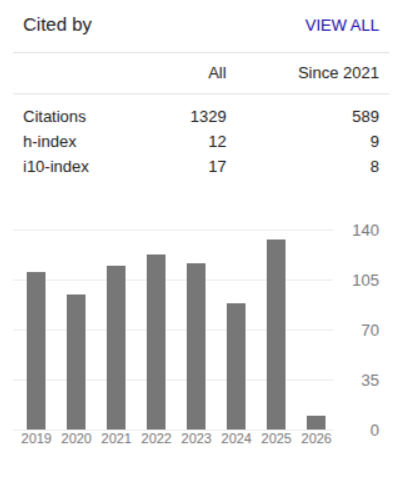
\includegraphics[
%    width=0.9\textwidth,
%    height=0.35\textheight,
%    keepaspectratio
%  ]{Scholar_Citations_2026-01-25T16-35-08.png}

 % \vspace{0.5\baselineskip}
 % {\small\itshape Google Scholar citation metrics (captured 25 January 2026).}
%\end{center}

\subsection*{\textbf{Books}}
\cvitem{Summary}{\textit{O’Donnell has published monographs, editions, and edited collections with Cambridge University Press, Boydell \& Brewer/Medieval Academy of America, and the University of Alberta Press. His edition of} Cædmon's Hymn \textit{(2005) was honorable mention for most distinguished critical edition (2007, MLA) and reprinted in an internet edition in 2018 (SEENET).}}

\cvitem{[3]}{rs Bordalejo, Barbara and \textbf{Daniel Paul O’Donnell}, eds. Contracted/Under review 2026. \textit{The Unessay Across the Disciplines: Practical Advice from Instructors in the Humanities, Social Sciences, and STEM}. University of Alberta Press.}
\cvitem{}{\textit{Collection of contributions exploring the use and impact of the "unessay" from teachers and researchers in English, History, Anthropology, Political Science, Biology, Medical Education, and Writing Studies/Study of Teaching and Learning. Fourteen chapters. Seventeen authors (one student). 78,500 words.}}

\cvitem{[2]}{rs Eve, Martin Paul, Cameron Neylon, \textbf{Daniel Paul O’Donnell}, Samuel Moore, Robert Gadie*, Victoria Odeniyi*, and Shahina Parvin*. 2020. \textit{Reading Peer Review: PLOS ONE and Institutional Change in Academia}. Cambridge: Cambridge University Press. \textsc{doi}: \url{https://doi.org/10.1017/9781108783521}. ISBN: 9781108486637 (hardback); 9781108783521 (ebook).}
\cvitem{}{%
  \textbf{Review:}
  \begin{itemize}
    \item \textit{Public Understanding of Science} 31.7 (2022): 892--894.
  \end{itemize}
}

\cvitem{[1]}{r \textbf{O’Donnell, Daniel Paul}. 2005. \textit{Cædmon’s Hymn: A Multimedia Study, Edition and Archive}. SEENET A.8. Cambridge: Medieval Academy of America and D.S. Brewer. xxii + 261~pp. + CD-ROM. Internet reprint (2018): \url{https://caedmon.seenet.org/}. Codebase \textsc{doi}: \url{https://doi.org/10.5281/zenodo.1198856}.}
\cvitem{}{%
  \textbf{Prize:}
  \begin{itemize}
    \item 2007 MLA Distinguished Scholarly Edition Prize (honourable mention).
  \end{itemize}
}
\cvitem{}{%
  \textbf{Reviews:}
  \begin{itemize}
    \item \textit{e-data\&research} 1 (2006): 1.
    \item \textit{Medium Aevum} 75 (2006): 356--357.
    \item \textit{Old English Newsletter} 40.1 (2006).
    \item \textit{Speculum} 82 (2007): 223--224.
    \item \textit{Journal of Ecclesiastical History} 58 (2007): 120--121.
    \item \textit{Early Medieval Europe} 15 (2007): 466--469.
    \item \textit{Textual Cultures} 2 (2007): 139--142.
    \item \textit{JEGP} 107.2 (2008): 248--251.
    \item \textit{Digital Medievalist} 5 (2009).
    \item \textit{Leeds Medieval Studies} 3 (2023).
  \end{itemize}
}
\cvitem{}{ %
  \textbf{Extended scholarly discussions} (other than reviews)\textbf{:}
  \begin{itemize}
    \item Katherine O'Brien O'Keeffe, “The Architecture of Old English Editions,” in \textit{Probable Truth: Editing Medieval Texts from Britain in the Twenty-First Century}, ed. Vincent Gillespie and Anne Hudson, 73--90. Turnhout: Brepols.
    \item Daniel Sondheim, Geoffrey Rockwell, Stan Ruecker, Mihaela Ilovan, Luciano Frizzera, and Jennifer Windsor. 2016. “Scholarly Editions in Print and on the Screen: A Theoretical Comparison.” \textit{Digital Studies / Le Champ Numérique}.
  \end{itemize}
}

\subsection*{\textbf{Articles and Chapters (Traditional)}}
\cvitem{Summary}{\textit{O’Donnell has published regularly as both a sole author and as part of teams in traditional scholarly venues including peer-reviewed journals and essay collections. In recent years, his authorship teams have regularly included graduate, and even undergraduate, student authors.}}

\cvitem{[46]}{rs Grandfield, Virgil, Davide Pafumi*, \textbf{Daniel Paul O’Donnell}, Frank Onuh*. Accepted 2026. "Insights regarding The “Subeditor Model”: Integrating Apprenticeship into Editorial Decision-Making for Acquiring Scholarly Communication Skills." \textit{Insights}. At press.}
\cvitem{[45]}{rs Bordalejo, Barbara, Davide Pafumi*, Morgan S. Pearce*, \textbf{Daniel Paul O’Donnell}. 2025. "Adapting a Research Tool for Teaching in a Post-Pandemic World: Textual Communities and Critical Digital Pedagogy in the Context of a Comprehensive Liberal Arts Research University." \textit{Digital Humanities Quarterly} 19.2. \url{https://www.digitalhumanities.org/dhq/vol/19/2/000787/000787.html}.}
\cvitem{[44]}{rs Davide Pafumi*, Frank Onuh*, AKM Iftekhar Khalid*, Morgan Pearce*, Barbara Bordalejo, \textbf{Daniel Paul O’Donnell}. 2025. “Scarlet Cloak and the Forest Adventure: A preliminary study of the impact of AI on commonly used writing tools.” \textit{International Journal of Educational Technology in Higher Education} 22.6. \textsc{doi}: \url{https://doi.org/10.1186/s41239-025-00505-5}.}
\cvitem{[43]}{ri \textbf{O’Donnell, Daniel Paul}. 2021. “‘I heard he sang a good song’: Caedmon’s inspiration and medieval dream theory.” In: \textit{Sogni, visioni e profezie nella letteratura germanica medievale}, edited by Roberto Rosselli Del Turco. Bibliotheca Germanica. Studi e testi 48. Allessandria: Edizioni del l’Orso, pp. 147–172.}
\cvitem{[42]}{r Heather Bliss, Inge Genee, Marie-Odile Junker, \textbf{Daniel Paul O’Donnell}. 2020. “‘Credit Where Credit Is Due’: Authorship and Attribution in Algonquian Language Digital Resources.” \textit{IDEAH} 1.1. Author order: Alphabetical. \textsc{doi}: \url{https://doi.org/10.21428/f1f23564.3d64b2ed}.}
\cvitem{[41]}{r \textbf{O’Donnell, Daniel Paul}. 2020. “Critical Mass: The Listserv and the Early Online Community as a Case Study in the Unanticipated Consequences of Innovation in Scholarly Communication.” In: \textit{Digital Technology and the Practices of Humanities Research}, edited by Jennifer Edmond. Cambridge: Open Book Publishers, pp. 184–206. \textsc{doi}: \url{https://doi.org/10.5281/zenodo.3633429}.}
\cvitem{[40]}{r \textbf{O’Donnell, Daniel Paul}. 2019. “All along the Watchtower: Intersectional diversity as a core intellectual value in the Digital Humanities.” In: \textit{Intersectionality in Digital Humanities}, edited by Barbara Bordalejo and Roopika Risam. Amsterdam: ARC. \textsc{doi}: \url{https://doi.org/10.5281/zenodo.3580235}.}
\cvitem{[39]}{rs Paul Esau*, Carey Viejou*, Sylvia Chow*, Kimberly Dohms*, Steve Firth*, Jarret McKinnon*, Dorethea Morrison*, Reed Parsons*, Courtney Rieger*, Vanja Spiric*, Elaine Toth*, Kayla Ueland*, Rumi Graham, \textbf{Daniel Paul O’Donnell}. 2018. “‘Let’s Start a Journal!’: The Multidisciplinary Graduate Student Journal as Educational Opportunity.” \textit{The Journal of Electronic Publishing (JEP)} 21.1. Corresponding author. \textsc{doi}: \url{https://doi.org/10.3998/3336451.0021.109}.}
\cvitem{[38]}{i \textbf{O’Donnell, Daniel Paul}, Matteo Callieri, Marco Dellepiane, Catherine Karkov, Dot Porter, Roberto Rosselli Del Turco. 2018. “Archaeology in the Study: Scanning Anglo-Saxon Artifacts in the Visionary Cross Project.” \textit{Wiðowinde} 185 (Spring), pp. 21–27. \textsc{doi}: \url{https://doi.org/10.5281/zenodo.1208167}.}
\cvitem{[37]}{rs \textbf{O’Donnell, Daniel Paul}, Carey Viejou*, Sylvia Chow*, Kimberly Dohms*, Paul Esau*, Steve Firth*, Rumi Graham. 2018. “Zombie Journals: Designing a Technological Infrastructure for a Precarious Graduate Student Journal.” \textit{Scholarly and Research Communication} 9.2. Corresponding author. \textsc{doi}: \url{https://doi.org/10.22230/src.2018v9n2a296}.}
\cvitem{[36]}{r Samuel Moore*, Cameron Neylon, Martin Paul Eve, \textbf{Daniel Paul O’Donnell}, Damian Pattinson. 
2017. “‘Excellence R Us’: University Research and the Fetishisation of Excellence.” \textit{Palgrave Communications} 3 (January). 
Author order: Random. \textsc{doi}: \url{https://doi.org/10.1057/palcomms.2016.105}.
\begin{itemize}
  \item This paper is the top publication by downloads and citations in the Nature imprint \textit{Humanities and Social Sciences Communications} (\href{https://www.nature.com/articles/palcomms2016105/metrics}{see article metrics}).
  \item It was also selected by the editors as one of the \href{https://www.nature.com/collections/dhhcjffjhb}{top fifty publications of the journal's first decade}.
\end{itemize}}
\cvitem{[35]}{r Tennant, Jonathan P., Jonathan M. Dugan,... \textbf{Daniel Paul O’Donnell} [38th author],... and others. 2017. “A Multi-Disciplinary Perspective on Emergent and Future Innovations in Peer Review.” \textit{F1000Research} 6.1151. Author order: Based on date of first edit. \textsc{doi}: \url{https://doi.org/10.12688/f1000research.12037.2}.}
\cvitem{[34]}{r Robin Champieux, Bianca Kramer, Jeroen Bosman, Ian Bruno, Amy Buckland, Sarah Callaghan, Chris Chapman, Stephanie Hagstrom, MaryAnn E. Martone, \textbf{Daniel Paul O’Donnell}. 2016. “Finding the Principles of the Commons: A Report of the Force11 Scholarly Communications Working Group.” \textit{Collaborative Librarianship} 8.2. \url{http://digitalcommons.du.edu/collaborativelibrarianship/vol8/iss2/5}.}
\cvitem{[33]}{rs Heather Hobma*, \textbf{Daniel Paul O’Donnell}, Catherine Karkov, Sally Foster, James Graham, Wendy Osborn, Roberto Rosselli Del Turco, Robert Broatch, Susan Broatch, Marco Callieri, Matteo Dellepiane. 2016. “Modern impact on the fabric of the Ruthwell Cross.” \textit{OEN} 46.1. Corresponding author. \url{http://www.oenewsletter.org/OEN/issue/ruthwell.php}.}
\cvitem{[32]}{r Bianca Kramer, Jeroen Bosman, Marcin Ignac, Christina Kral, Tellervo Kalleinen, Pekko Koskinen, Ian Bruno, Amy Buckland, Sarah Callaghan, Robin Champieux, Chris Chapman, Stephanie Hagstrom, MaryAnn Martone, Fiona Murphy, \textbf{Daniel Paul O’Donnell}. 2016. “Defining the Scholarly Commons – Reimagining Research Communication.” \textit{Research Ideas and Outcomes} 2 (May), e9340. \textsc{doi}: \url{https://doi.org/10.3897/rio.2.e9340}.}
\cvitem{[31]}{i \textbf{O’Donnell, Daniel Paul}. 2016. “The Bird in Hand: Humanities Research in the Age of Open Data.” In: \textit{The State of Open Data}, edited by Figshare. London: Digital Science, pp. 34–35. \textsc{doi}: \url{https://doi.org/10.5281/zenodo.1470821}.}
\cvitem{[30]}{rs \textbf{O’Donnell, Daniel Paul}, Jessica Bay*, Emma Dering*, Matt Gal*, Virgil Grandfield*, Heather Hobma*, Gurpreet Singh*. 2016. “The Third Academic Freedom.” \textit{Light on Teaching}, pp. 4–9. Corresponding author. \textsc{doi}: \url{https://doi.org/10.5281/zenodo.3596098}.}
\cvitem{[29]}{rs Chiara Leoni*, Marco Callieri, Matteo Dellepiane, \textbf{Daniel Paul O’Donnell}, Roberto Rosselli Del Turco, Roberto Scopigno. 2015. “The Dream and the Cross: a 3D scanning project to bring 3D content in a digital edition.” \textit{Journal on Computing and Cultural Heritage}. \textsc{doi}: \url{https://doi.org/10.1145/2686873}.}
\cvitem{[28]}{r \textbf{O’Donnell, Daniel Paul}, Alex Gil, Katherine Walters, Neil Fraistat. 2015. “Only Connect: The Globalization of the Digital Humanities.” In: \textit{A New Companion to Digital Humanities}, edited by Susan Schreibman, Ray Siemens, and John Unsworth. Wiley, pp. 493–510. \textsc{doi}: \url{https://doi.org/10.1002/9781118680605.ch34}.}
\cvitem{[27]}{rs \textbf{O’Donnell, Daniel Paul}, Heather Hobma*, Sandra Cowan, Gillian Ayers*, Jessica Bay*, Marinus Swanepoel, Wendy Merkley, Kelaine Devine*, Emma Dering*, Inge Genee. 2015. “Aligning Open Access Publication with the Research and Teaching Missions of the Public University.” \textit{Journal of Electronic Publishing} 18.3. Corresponding author. \textsc{doi}: \url{https://doi.org/10.3998/3336451.0018.309}.}
\cvitem{[26]}{r \textbf{O’Donnell, Daniel Paul}. 2013. “‘I certainly have subjects in my mind’: The Diary of Anne Frank as Bildungsroman.” \textit{Canadian Journal of Netherlandic Studies} 32, pp. 49–88. \textsc{doi}: \url{https://doi.org/10.5281/zenodo.3596110}.}
\cvitem{[25]}{r \textbf{O’Donnell, Daniel Paul}. 2012. “Move Over: Learning to Read (and Write) with Novel Technology.” \textit{Scholarly and Research Communication} 3.4. \textsc{doi}: \url{https://doi.org/10.22230/src.2012v3n4a68}.}
\cvitem{[24]}{r \textbf{O’Donnell, Daniel Paul}. 2010. “Different Strokes, Same Folk: Designing the Multi-form Digital Edition.” \textit{Literature Compass} 7.2. \textsc{doi}: \url{https://doi.org/10.1111/j.1741-4113.2009.00683.x}.}
\cvitem{[23]}{r Stuart Lee and \textbf{Daniel Paul O’Donnell}. 2009. “From Manuscript to Computer.” In: \textit{Working with Anglo-Saxon Manuscripts}, edited by Gale R. Owen-Crocker. Exeter: Exeter UP, pp. 253–284.}
\cvitem{[22]}{r \textbf{O’Donnell, Daniel Paul}. 2009a. “Back to the future: What digital editors can learn from print editorial practice.” \textit{Literary and Linguistic Computing} 24, pp. 113–125. \textsc{doi}: \url{https://doi.org/10.1093/llc/fqn039}.}
\cvitem{[21]}{i \textbf{O’Donnell, Daniel Paul}. 2009b. “Byte me: Technological Education and the Humanities.” \textit{Heroic Age} 12. \url{http://www.mun.ca/mst/heroicage/issues/12/em.php}.}
\cvitem{[20]}{ri Gabriel Bodard, \textbf{Daniel Paul O’Donnell}. 2008. “We are all together: On publishing a Digital Classicist issue of the Digital Medievalist journal.” \textit{Digital Medievalist} 4. Corresponding author. \textsc{doi}: \url{https://doi.org/10.16995/dm.18}.}
\cvitem{[19]}{i \textbf{O’Donnell, Daniel Paul}. 2008. “Resisting The Tyranny of the Screen, or, Must a Digital Edition be Electronic?” \textit{Heroic Age} 11. \url{http://www.heroicage.org/issues/11/em.php}.}
\cvitem{[18]}{r \textbf{O’Donnell, Daniel Paul}. 2007a. “Disciplinary impact and technological obsolescence in digital medieval studies.” In: \textit{A Companion to Digital Literary Studies}, edited by Ray Siemens and Susan Schreibman. Cambridge: Blackwell. \textsc{doi}: \url{https://doi.org/10.1002/9781405177504.ch3}.}
\cvitem{[17]}{i \textbf{O’Donnell, Daniel Paul}. 2007b. “If I were ‘You’: How academics can stop worrying and learn to love ‘the encyclopedia that anyone can edit.’” \textit{Heroic Age} 10. \url{http://www.heroicage.org/issues/10/em.html}.}
\cvitem{[16]}{r \textbf{O’Donnell, Daniel Paul}. 2007c. “Material differences: The place of Cædmon’s Hymn in the history of Anglo-Saxon vernacular poetry.” In: \textit{Cædmon’s Hymn and Material Culture in the World of Bede}, edited by Allen J. Frantzen and John Hines. Morgantown VA: West Virginia University Press, pp. 15–50.}
\cvitem{[15]}{i \textbf{O’Donnell, Daniel Paul}. 2005a. “O Captain! My Captain! Using technology to guide readers through an electronic edition.” \textit{Heroic Age} 8. \url{http://www.heroicage.org/issues/8/em.html}.}
\cvitem{[14]}{i \textbf{O’Donnell, Daniel Paul}. 2005b. “The Ghost in the Machine: Revisiting an Old Model for the Dynamic Generation of Digital Editions.” \textit{HumanIT} 8.1, pp. 51–71. \textsc{doi}: \url{https://doi.org/10.5281/zenodo.3596125}.}
\cvitem{[13]}{r \textbf{O’Donnell, Daniel Paul}. 2004a. “Bede’s Strategy in Paraphrasing Cædmon’s Hymn.” \textit{JEGP} 103, pp. 417–433.}
\cvitem{[12]}{r \textbf{O’Donnell, Daniel Paul}. 2004b. “Numeric and Geometric Patterning in Cædmon’s Hymn.” \textit{ANQ} 17, pp. 3–12.}
\cvitem{[11]}{i \textbf{O’Donnell, Daniel Paul}. 2004c. “The Digital Medievalist Project.” \textit{Old English Newsletter} 37, pp. 19–21.}
\cvitem{[10]}{i \textbf{O’Donnell, Daniel Paul}. 2004d. “The Doomsday Machine, or, ‘If you build it, will they still come ten years from now?’: What Medievalists working in digital media can do to ensure the longevity of their research.” \textit{Heroic Age} 7. \url{http://www.heroicage.org/issues/7/ecolumn.html}.}
\cvitem{[9]}{r \textbf{O’Donnell, Daniel Paul}. 2003. “‘Pioneers! O Pioneers!’: Some Electronic Editing Do’s and Don’ts from Stijn Streuvels’s \textit{De teleurgang van den Waterhoek}.” \textit{Literary and Linguistic Computing}.}
\cvitem{[8]}{r \textbf{O’Donnell, Daniel Paul}. 2002a. “Junius’s Knowledge of the Old English Poem \textit{Durham}.” \textit{Anglo-Saxon England} 30, pp. 231–245.}
\cvitem{[7]}{r \textbf{O’Donnell, Daniel Paul}. 2002b. “The Accuracy of the St. Petersburg Bede.” \textit{Notes and Queries} 247, pp. 4–6.}
\cvitem{[6]}{r \textbf{O’Donnell, Daniel Paul}. 2001. “Fish and Fowl: Generic Expectations and the Relationship between the Old English \textit{Phoenix} poem and Lactantius’s \textit{De ave phoenice}.” In: \textit{Germanic Texts and Latin Models: Medieval Reconstructions}, edited by K.E. Olsen, A. Harbus, and T. Hofstra. Germania Latina IV. Mediaevalia Groningana, n.s. 2. Leuven, Paris and Sterling, VA: Peeters, pp. 157–171.}
\cvitem{[5]}{r \textbf{O’Donnell, Daniel Paul}. 1999. “Hædre and Hædre Gehogode (\textit{Solomon and Saturn} line 62b and \textit{Resignation} line 63a).” \textit{Notes and Queries} 244, pp. 312–316.}
\cvitem{[4]}{r \textbf{O’Donnell, Daniel Paul}. 1998. “The Spirit and the Letter: Literary Embellishment in Old Frisian Legal Texts.” \textit{Amsterdamer Beiträge zur älteren Germanistik} 49, pp. 245–256.}
\cvitem{[3]}{r \textbf{O’Donnell, Daniel Paul}. 1996. “A Northumbrian Version of ‘Cædmon’s Hymn’ (eordu-recension) in Brussels Bibliothèque Royale Manuscript 8245–57 ff.62r\textsuperscript{2}–v\textsuperscript{1}: Identification, Edition, and Filiation.” In: \textit{Beda Venerabilis: Historian, Monk and Northumbrian}, edited by L.A.R.J. Houwen and A.A. MacDonald. Groningen: Egbert Forsten, pp. 139–166.}
\cvitem{[2]}{r \textbf{O’Donnell, Daniel Paul}. 1995. “Schoolbook Design in the Fifteenth Century.” \textit{The Yale University Library Gazette} 70, pp. 23–38.}
\cvitem{[1]}{r \textbf{O’Donnell, Daniel Paul}. 1991. “The Collective Sense of Concrete Singular Nouns in \textit{Beowulf}: Emendations of Sense.” \textit{Neuphilologische Mitteilungen} 92, pp. 433–440.}

\subsection*{\textbf{Research Lectures}}

\cvitem{[134]}{rs Khalid, AKM Iftekhar*, Frank Onuh*, Barbara Bordalejo, and \textbf{Daniel Paul O’Donnell}. 2025. “Choose Your Poison: The Company Store vs. Data Colonialism as a Means of Understanding the Exploitative Potential of Asymmetry in Data Collection and Service Provision.” DH 2025, Lisbon, July 18. https://dh2025.adho.org/browse-the-program-agenda/.}
\cvitem{[133]}{rs McKnight, Jocelyn Lilly**, \textbf{Daniel Paul O’Donnell}, Roberto Rosselli Del Turco, Barbara Bordalejo. 2025. "I’m Looking Through You: Building the Interface for a 3D Edition for The Visionary Cross Project." Session 5B: "Space and Sound." Congress 2025 - CSDH/SCHN, Toronto, June 1.}
\cvitem{[132]}{rs McKnight, Jocelyn Lily**, Davide Pafumi*, \textbf{Daniel Paul O’Donnell}. 2025. "Working with Historical Textual Data: Preliminary Results from Applying Survival Analysis to the Old English Poetic Corpus." Session 5B: "Literary DH." Congress 2025 - CSDH/SCHN, Toronto, May 31.}
\cvitem{[131]}{rs Woods, Nathan D., Davide Pafumi*, Barbara Bordalejo, \textbf{Daniel Paul O’Donnell}. 2025. "Rethinking the Advancement of Humanities Knowledge: Innovation and Change in the Humanities Data Ecosystem." Session 3A: "DH Communities." Congress 2025 - CSDH/SCHN, Toronto, May 31.}
\cvitem{[130]}{rs Onuh, Frank*, AKM Iftekhar Khalid*, Barbara Bordalejo, and \textbf{Daniel Paul O’Donnell}. “Choose Your Poison: Data Colonialism or Company Town?”. Session 1B "Digital Capitalism." Congress 2025 - CSDH/SCHN, Toronto, May 30. https://doi.org/10.5281/zenodo.15548208.}
\cvitem{[129]}{is \textbf{O’Donnell, Daniel Paul}, Barbara Bordalejo, Davide Pafumi*, and Jocelyn McKnight**. 2025. "Éloge de la variante? Working with Old English textual variants for 30 years." Norma variazione identità. May 30. Rome/Online. https://doi.org/10.5281/zenodo.15549269}
\cvitem{[128]}{i \textbf{O’Donnell, Daniel Paul}. 2024. “Academic Freedom, Privilege, and Intersectionality.” July 29.  Force11 Scholarly Communications Institute (FSCI), Los Angeles. Zenodo. https://doi.org/10.5281/zenodo.13121345}
\cvitem{[127]}{rs Bordalejo, Barbara, Davide Pafumi*, Frank Onuh, AKM Iftekhar Khalid, and \textbf{Daniel Paul O’Donnell}. 2024. “Scarlet Cloak and the Forest Adventure: The Issue of False Positives in AI Detection Tools.” June 17. Congress of the Humanities and Social Sciences (CSDH/SCHN). Montreal. https://doi.org/10.5281/zenodo.12011536.}
\cvitem{[126]}{rs Bordalejo, Barbara, Davide Pafumi*, Morgan Slayde Pearce*, and \textbf{Daniel Paul O’Donnell}. 2024. “Adapting a Research Tool for Teaching in a Post-Pandemic World.” June 17. Congress of the Humanities and Social Sciences (CSDH/SCHN). Montreal.  https://doi.org/10.5281/zenodo.12018101.}
\cvitem{[125]}{r \textbf{O’Donnell, Daniel Paul}, Barbara Bordalejo, and Nathan D. Woods. 2024. “Data in/And Mediaeval Studies.” International Congress on Medieval Studies. Kalamazoo. May 11. https://doi.org/10.5281/zenodo.11179271.}
\cvitem{[124]}{r Woods, Nathan, Barbara Bordalejo, and \textbf{Daniel Paul O’Donnell}. 2023. “Data Problems in the Humanities, or ‘When Everybody Is Special, No One Is’?” October 3. https://doi.org/10.5281/zenodo.8403789.}
\cvitem{[123]}{r Bordalejo, Barbara, \textbf{Daniel Paul O’Donnell}, and Nathan Woods. 2023. “The Implications of Multiple Hierarchies for the Future of Humanities Data: Or, What Is a Markup Language, Actually?” October 5. https://doi.org/10.5281/zenodo.8411165.}
\cvitem{[122]}{r \textbf{O’Donnell, Daniel Paul}, Barbara Bordalejo, and Nathan Woods. 2023. “Representational Data:  A Case Study.” May 30.  Congress of the Social Sciences and Humanities. https://doi.org/10.5281/zenodo.7986430.}
\cvitem{[121]}{r \textbf{O’Donnell, Daniel Paul}, Barbara Bordalejo, Nathan Woods, Roberto Rosselli Del Turco. 2022. “Small Data projects/Big Data research: contemporary problems and historical solutions.” DH 2022 (Tokyo/online). July 28. https://doi.org/10.5281/zenodo.6857202.}
\cvitem{[120]}{r \textbf{O’Donnell, Daniel Paul}. 2022. “‘Good things come in small packets’: Investigating Humanities Research Data Practices: A Community of Practice Approach.” FSCI 2022. Lightning Talks. July 25-29. https://doi.org/10.5281/zenodo.6902821.}
\cvitem{[119]}{r \textbf{O’Donnell, Daniel Paul}. 2022. “REPO: Reimagining Educational Practices for Open 2020-2021.” FSCI 2022. Force11 Working Group Bazaar. July 25. https://doi.org/10.5281/zenodo.6902861.}
\cvitem{[118]}{r \textbf{O’Donnell, Daniel Paul}, Barbara Bordalejo, Nathan Woods, Roberto Rosselli Del Turco. 2022. “Small Data Management in Humanities and Cultural Heritage Projects.” DH Unbound. May 17. https://doi.org/10.5281/zenodo.6773410.}
\cvitem{[117]}{i \textbf{O’Donnell, Daniel Paul}. 2022. “Thinking about CARE principles in the Digital Humanities.  Why CARE may not be only a matter for researchers working with indigenous peoples.” RDA-DU. Online. Feb 21.}
\cvitem{[116]}{i \textbf{O’Donnell, Daniel Paul}. 2021. ''Thinking about CARE principles in the Digital Humanities. Why CARE may not be only a matter for researchers working with indigenous peoples.” DARIAH Friday Frontiers. Online. October. France. October 8.}
\cvitem{[115]}{i \textbf{O’Donnell, Daniel Paul}, Rosselli Del Turco R. 2020. 'Methods and tools to build a web-based edition on the basis of FAIR/OA data'. Assemblée Générale du consortium Cahier. France. November 27. https://cahier.hypotheses.org/5384.}
\cvitem{[114]}{i \textbf{O’Donnell, Daniel Paul}. (2020, August). How to make a manifesto… and not: Principles of the Scholarly Commons as Case History (Version Presentation). Presented at the Force11 Scholarly Communication Institute 2020 Online (FSCI 2020 Online), Online: Zenodo. http://doi.org/10.5281/zenodo.3979532.}
\cvitem{[113]}{r Bordalejo, Barbara, Folgert Karsdorp, \textbf{Daniel Paul O’Donnell}, Basten Stokhuyzen, and Karina Van Dalen-Oskam. 2020. “Check Your Privilege: The Digital Privilege Game.” Congress 2020 (online). June 5. Published in Building Community Online. https://hcommons.org/deposits/item/hc:30179.}
\cvitem{[112]}{i \textbf{O’Donnell, Daniel Paul}, and Virgil Grandfield. 2020. “The Lethbridge Journal Incubator: A Collaborative Student-Expert Open Access Publishing Model.” Open Publishing Fest. May 28. https://doi.org/10.5281/zenodo.3863022.}
\cvitem{[111]}{i \textbf{O’Donnell, Daniel Paul}. 2019. Publishing (and Forgetting) the Small or Medium-sized Scholarly Edition or Cultural Heritage Collection as Linked Open Data: Using Zenodo and Github to Publish the Visionary Cross Project. Winter Institute in Digital Humanities. IIT Gandhinagar. Palaj, India. December 20. https://zenodo.org/record/3586007. (Updated version of DH2019 presentation).}
\cvitem{[110]}{i \textbf{O’Donnell, Daniel Paul}. 2019. Small, thick, and slow: Towards an Open and FAIR data culture in the Humanities. Winter Institute in Digital Humanities. IIT Gandhinagar. Palaj, India. December 18. https://zenodo.org/record/3581520.}
\cvitem{[109]}{r \textbf{O’Donnell, Daniel Paul}. 2019. Publishing (and Forgetting) the Small or Medium-sized Scholarly Edition or Cultural Heritage Collection as Linked Open Data: Using Zenodo and Github to Publish the Visionary Cross Project. Digital Humanities 2019. Utrecht, Netherlands. July 10. https://zenodo.org/record/3586007.}
\cvitem{[108]}{i \textbf{O’Donnell, Daniel Paul}. 2019. Small, thick, and slow: Thinking about data and research publication in the Humanities in the age of Open and FAIR. Curtin University. Perth, Australia. November 25, 2019. https://zenodo.org/record/3554760.}
\cvitem{[107]}{i \textbf{O’Donnell, Daniel Paul}. 2018. The Nature of Humanities Data. Open Science Infrastructures for Big Cultural Data: International Advanced Masterclass. Plovdiv, Bulgaria. December 14. http://doi.org/10.5281/zenodo.2246390.}
\cvitem{[106]}{i \textbf{O’Donnell, Daniel Paul}. 2018. The Humanities and New Technologies: Exploring Digital Tools for Innovation and Development. Keynote address. 2nd Lagos Summer School in Digital Humanities. University of Lagos, Nigeria. October 2. https://doi.org/10.5281/zenodo.1443255.}
\cvitem{[105]}{i \textbf{O’Donnell, Daniel Paul}. 2018. Open Access/Open Science and the Humanities on a Cross-Regional Basis. Invited lecture. Elizade University, Ilara-Mokin, Nigeria. Sept. 28. https://doi.org/10.5281/zenodo.1455735.}
\cvitem{[104]}{i \textbf{O’Donnell, Daniel Paul}. 2018. Sometimes a poet is just a poet: Reading Bede reading Cædmon’s inspiration in light of Germanic Tradition and cultural analogues. Invited lecture. XIX Seminario Avanzato in Filologia Germanica "Sogni, Visioni e Profezie nella letteratura Germanica medievale. Università degli studi di Torino. Sept. 18. http://doi.org/10.5281/zenodo.2222396.}
\cvitem{[103]}{r \textbf{O’Donnell, Daniel Paul}. 2018. Open in the Digital Humanities. Some thoughts on cross-disciplinary similarity and difference. DH 2018. Mexico City.}
\cvitem{[102]}{i \textbf{O’Donnell, Daniel Paul}. 2018. Le goût de la mer: Teaching Research. Invited lecture. University of Saskatchewan. May 8.}
\cvitem{[101]}{isc Bar-Sinai, Michael, Jeroen Bosman, Ian Bruno, Chris Chapman, Bastian Greshake Tzovaras, Stephanie Hagstrom, Nate Jacobs*, Bianca Kramer, Maryann Martone, Fiona Murphy, \textbf{Daniel Paul O’Donnell} [alphabetical order]. 2018. “Hier stehe ich! Operationalising conviction in the Scholarly Commons.” McGill. April 4.}
\cvitem{[100]}{i \textbf{O’Donnell, Daniel Paul} 2017. 'How to Start an Open Access Journal'. Open Access Week. Lethbridge. Canada.}
\cvitem{[99]}{rs Heather Bliss*, Inge Genee, Marie Odile Junker, and \textbf{Daniel Paul O’Donnell}, 2017. “Credit where credit is due”: How to handle attribution, copyright, and intellectual property in on-line digital resources for Algonquian languages.” The Algonguin Conference, Université de Montréal. October 28.}
\cvitem{[98]}{i \textbf{O’Donnell, Daniel Paul}. 2017. Humanities in the Age of Technology [Keynote]. 1st Lagos Summer School in Digital Humanities. University of Lagos, Nigeria. July 11.}
\cvitem{[97]}{rs Esau, Paul*, Carey Viejou*, Sylvia Chow*, Jarret McKinnon*, Reed Parsons*, and \textbf{Daniel Paul O’Donnell}. 2017. First World Problems: Publishing a Graduate Student Journal in the Anglophone Global North Using Minimal Computing Techniques. Session 9a: Open Access/Social Scholarship. Canadian Society for Digital Humanities/Société canadienne des humanités numériques. Congress 2017. Ryerson University, Toronto. May 31.}
\cvitem{[96]}{rsc \textbf{O’Donnell, Daniel Paul}, Dot Porter, Roberto Rosselli Del Turco, Gurpreet Singh*. 2017. Let’s Get Nekkid! Stripping the User Experience to the Bare Essentials. Sesion 5a: Digital Editions. Canadian Society for Digital Humanities/Société canadienne des humanités numériques. Congress 2017. Ryerson University, Toronto. May 30.}
\cvitem{[95]}{rs Esau, Paul*, Carey Viejou*, and \textbf{Daniel Paul O’Donnell}. 2017. Publishing the Unpublishable: The Story of a Graduate Journal and a University that Wouldn’t Submit to it. Canadian Association of Learned Journals. Congress 2017. Ryerson University, Toronto. May 27.}
\cvitem{[94]}{i \textbf{O’Donnell, Daniel Paul}. 2017. “The Bird in Hand: Humanities research in the age of open data.” Research Data Management Interdisciplinary Panel Discussion. Centre for the Study of Scholarly Communication. University Library. University of Lethbridge. March 16.}
\cvitem{[93]}{i \textbf{O’Donnell, Daniel Paul}. 2017. “When is infrastructure really a project?.” Open Scientific Infrastructure: in Search of a Development Model. Gaidar Forum: Russia and the World: The Choice of Priorities. Russian Presidential Academy of National Economy and Public Administration. Moscow. January 14.}
\cvitem{[92]}{i \textbf{O’Donnell, Daniel Paul}. 2016. “Length and Breadth: Why diversity is a core intellectual value in the Digital Humanities.” Intersectionality in Digital Humanities Conference. KU Leuven. September 15.}
\cvitem{[91]}{r \textbf{O’Donnell, Daniel Paul}. 2016. All along the Watchtower: An interdisciplinary approach to understanding the importance technical, disciplinary, and interpersonal diversity within the Digital Humanities. DH 2016. Krakow. July 12.}
\cvitem{[90]}{rs \textbf{O’Donnell, Daniel Paul} and Shelaigh Brantford**. 2016. “The tip of the iceberg: Transparency and diversity in contemporary DH.” Congress 2016. University of Calgary. June 1. Summarised by Geoffrey Rockwell at http://philosophi.ca/pmwiki.php/Main/CSDH-CGSA2016.}
\cvitem{[89]}{Bosman, Jeroen, Ian Bruno, Amy Buckland, Sarah Callaghan, Robin Champieux, Chris Chapman, Stephanie Hagstrom, Bianca Kramer, MaryAnn Martone, \textbf{Daniel Paul O’Donnell}. 2016. Scholarly Commons Working Group Webinar. Force11.org. May 24. https://www.force11.org/group/SCWG/May24webinar}
\cvitem{[88]}{i \textbf{O’Donnell, Daniel Paul}. 2016. “All Growed Up: Preparing Gold Open Access Journals for a Post-Incubator Life. Some lessons on transitions and new beginnings.” OA@UNT. University of North Texas. May 20.}
\cvitem{[87]}{i \textbf{O’Donnell, Daniel Paul}. 2016. The Visionary Cross Project and the Lethbridge Journal Incubator. Lethbridge SSHRC Showcase. April 29, 2016.}
\cvitem{[86]}{ir \textbf{O’Donnell, Daniel Paul}. 2016. Est ce qu’il y a de hors-edition? or, Can you edit everything? MLA 2016 Austin. Session 215 Editing Unruly Objects. January 8.}
\cvitem{[85]}{rs Moore, Samuel*, Damian Pattison, Cameron Neylon, \textbf{Daniel Paul O’Donnell}. 2015. The Quality of Qualities. Excellence and Soundness in Scholarly Communication. Mellon Triangle Scholarly Communication Workshop. Durham/Raleigh. UNC. October 12-16.}
\cvitem{[84]}{r Ortega, Élika, Alex Gil, \textbf{Daniel Paul O’Donnell}. 2015. “Psst! An Informal Approach to Expanding the Linguistic Range of the Digital Humanities.” Digital Humanities 2015. Melbourne. July 1.}
\cvitem{[83]}{rs \textbf{O’Donnell, Daniel Paul}, Gurpreet Singh*, Rachel Hanks**, Roberto Rosselli Del Turco. 2015. “The Old Familiar Faces: On the Consumption of Digital Scholarship.” Digital Humanities 2015. Melbourne. July 2.}
\cvitem{[82]}{r \textbf{O’Donnell, Daniel Paul}. 2015. “Est ce qu’il y a de hors-edition? or, Can you edit everything?” Canadian Society for Digital Humanities. Congress of the Humanities and Social Sciences. Ottawa. June 3.}
\cvitem{[81]}{s \textbf{O’Donnell, Daniel Paul}, Rachel Hanks**, Gurpreet Singh*, Roberto Rosselli Del Turco. 2015. “The Old Familiar Faces: On the consumption of (digital) textual scholarship.” Highway 2 Conference, University of Lethbridge May 9.}
\cvitem{[80]}{r \textbf{O’Donnell, Daniel Paul}. 2015. “The 'Unessay': A new approach to not teaching composition.” Spark. University of Lethbridge. April 30.}
\cvitem{[79]}{i \textbf{O’Donnell, Daniel Paul}. 2015. ““If 'if's and 'and's were pots and pans...”: Aligning Open Access Publication with the Research and Teaching Missions of the Public University: The Case of the Lethbridge Journal Incubator.” Advancing Research Communication and Scholarship. Philadelphia. April 15.}
\cvitem{[78]}{i \textbf{O’Donnell, Daniel Paul}. 2015. “‘Living Out Loud: Public Humanities and an Eight Century Cross.” North Carolina State University. April 15.}
\cvitem{[77]}{i \textbf{O’Donnell, Daniel Paul}. 2015. “Critical Mass: Online Communities and the Advancement of Research Communication.” Maynooth University (Ireland). March 5.}
\cvitem{[76]}{i \textbf{O’Donnell, Daniel Paul}. 2015. “‘Living Out Loud: The Visionary Cross Project and the Public Humanities.” Maynooth University (Ireland). March 5.}
\cvitem{[75]}{i \textbf{O’Donnell, Daniel Paul}. 2015. “‘All Together Now...’ Mobilising the (digital) Humanities in the Information Age.” Brigham Young University. February 2.}
\cvitem{[74]}{i \textbf{O’Donnell, Daniel Paul}. 2015. “‘All Together Now...’ Mobilising the (digital) Humanities in the Information Age.” University of Balamand (Lebanon). January 16.}
\cvitem{[73]}{r \textbf{O’Donnell, Daniel Paul}. 2015. “First thing we do, let's kill all the authors. On subverting scientific and scholarly authorship.” Force 2015. Oxford. January 13.}
\cvitem{[72]}{i \textbf{O’Donnell, Daniel Paul}. 2014. “‘All Together Now...’ Mobilising the (digital) Humanities in the Information Age” Universität Basel, October 13. http://www.slideshare.net/caedmon/20141013-basel.}
\cvitem{[71]}{i \textbf{O’Donnell, Daniel Paul}, Alex Gil. “Globalisation.” Around the world. A worldwide collaborative conference on privacy and surveillance in the digital age. Hosted by the Kule Institute for Advanced Study. May 21, 2014. http://aroundtheworld.ualberta.ca/2014/06/ulethbridge-and-columbia/}
\cvitem{[70]}{i Rockwell, Geoffrey, Michael Sinatra, Susan Brown, Dean Irvine, Ray Siemens, Stefan Sinclair, \textbf{Daniel Paul O’Donnell}. “Problems to be solved in DigHum: The Large-Scale Digital Humanities. Opportunities and challenges of distributed large-scale data to the humanities.” GRAND Ottawa. May 14, 2014.}
\cvitem{[69]}{i \textbf{O’Donnell, Daniel Paul}, et al. “The Lethbridge Journal Incubator: A new business model for Open Access journal publication.” Elsevier Labs (Virtual presentation). February 18, 2014.}
\cvitem{[68]}{is Hobma, Heather* and \textbf{Daniel Paul O’Donnell}. “Living out loud: The Visionary Cross Project and the Public Humanities.” CMRS/ETRUS. University of Saskatchewan. Saskatoon. January 16, 2014.}
\cvitem{[67]}{is \textbf{O’Donnell, Daniel Paul}, et al. “Class 2.0: Digital technology and digital rhetorics in the undergraduate classroom.” Department of English, University of Saskatchewan. Saskatoon. January  15, 2014. Also presented to the Department of English, University of Lethbridge. February 7, 2014.}
\cvitem{[66]}{i \textbf{O’Donnell, Daniel Paul}, et al. “The Lethbridge Journal Incubator. Leveraging Open Access Publication to Increase the Training and Research Capacity of the University.” Western Humanities Associate 2013. University of California San Diego. November 1, 2013.}
\cvitem{[65]}{rs Leoni, Chiara*, Marco Callieri, Matteo Dellepiane, Roberto Rosselli del Turco, \textbf{Daniel Paul O’Donnell}, and Roberto Scopigno. Forthcoming. “The Dream and the Cross: A 3D-Referenced, Web-Based Digital Edition.” Digital Heritage International Conference 2013. Marseille. Monday, October 28, 2013. This also won best paper prize.}
\cvitem{[64]}{i \textbf{O’Donnell, Daniel Paul}. “This changes everything! The “Digital Turn” and the Institutional Practice of the Humanities.” I Seminário Internacional em Humanidades Digitais no Brasil. Universidade de São Paulo.  October 23, 2013.}
\cvitem{[63]}{r \textbf{O’Donnell, Daniel Paul}, et al. “The The Visionary Cross Project.” ISAS 2013 (International Society of Anglo-Saxonists). Trinity College and University College Dublin.  29 July, 2013.}
\cvitem{[62]}{\textbf{O’Donnell, Daniel Paul}, et al. “The Unessay, or, The Pedagogy of Screwing Around. A Digital Humanities Approach to Teaching Scholarly Writing.” Pedagogy Lightening Talks. Digital Humanities 2013. University of Nebraska. 17 July, 2013.}
\cvitem{[61]}{r \textbf{O’Donnell, Daniel Paul}. “Everything that Rises Must Converge: On the Convergence of Informational and Critical Approaches to Textual, Cultural, and Material Heritage.” Medieval Cultural, Textual, and Material Culture in the Digital Age. Leeds International Medieval Congress. University of Leeds. 1 July, 2013. Different Version also delivered to Social Digital Scholarly Editing 2013. University of Saskatoon. 11 July, 2013.}
\cvitem{[60]}{s r \textbf{O’Donnell, Daniel Paul}. “The end of history: A case study in the practice of digital popular knowledge mobilization.” Refereed Lecture. Immersive interpretation and the small cultural heritage site: the case of Ruthwell Kirk. Canadian Society for Digital Humanities. Victoria. 5 June, 2013.}
\cvitem{[59]}{r \textbf{O’Donnell, Daniel Paul}. “The Old Familiar Faces: On the consumption of (digital) textual scholarship.” Refereed Lecture. Social and Digital Editions. Canadian Society for Digital Humanities. Victoria. 3 June, 2013.}
\cvitem{[58]}{i \textbf{O’Donnell, Daniel Paul}. 2013. “The meteor has struck. The dust is in the air. Let’s leave the dinosaurs to their fate and concentrate on the mammals: Notes on the New Humanities.” Invited Keynote. Digging the Digital. Graduate Student Conference on the Digital Humanities. University of Alberta. April 5-6.}
\cvitem{[57]}{i \textbf{O’Donnell, Daniel Paul}. 2013. “New Business Models for Open Access Publication in the Humanities: The Lethbridge Journal Incubator.” Beyond the PDF2. Amsterdam. 19 March.}
\cvitem{[56]}{rs \textbf{O’Donnell, Daniel Paul}, Heather Hobma*. 2012. “Far From the Maddening Crowd: Digital Projects and the Ethics of Popular Knowledge Mobilization.” Havana. 12 December.}
\cvitem{[55]}{r \textbf{O’Donnell, Daniel Paul}, James Graham, Catherine E. Karkov, and Roberto Rosselli del Turco. 2012. "Is there a text in this edition? On the implications of multiple media and immersive technology for the future of the ‘scholarly edition’." European Society for Textual Scholarship (ESTS), Amsterdam. 23 November.}
\cvitem{[54]}{i \textbf{O’Donnell, Daniel Paul}. 2012. "The Lethbridge Journal Incubator: Aligning scholarly publishing with the teaching and research missions of a public university." Canadian Association of Learned Journals. Congress of the Federation of the Social Sciences and Humanities. Waterloo, Ontario. May 27.}
\cvitem{[53]}{i \textbf{O’Donnell, Daniel Paul}. 2012. "Markup and Metadata: An introduction to the power of XML and related technologies in humanities research applications." Pre-conference Workshop. Society for Digital Humanities/Société pour l’étude des médias interactifs. Congress of the Federation of the Social Sciences and Humanities. Waterloo, Ontario. May 25.}
\cvitem{[52]}{i \textbf{O’Donnell, Daniel Paul}. 2012. "abdah.org: Alberta Digital Arts and Humanities and Campus Alberta." Presentation to Campus Alberta Arts, Social Sciences, and Humanities. University of Calgary. May 11.}
\cvitem{[51]}{i \textbf{O’Donnell, Daniel Paul}. 2012. "Move Over: Learning to Read (and Write) with Novel Technology." MARCS: The Medieval and Renaissance Cultural Studies Research Group. University of  Calgary, March 15.}
\cvitem{[50]}{r \textbf{O’Donnell, Daniel Paul}. 2011. "'Nor doubted once': Editing Text and Context." INKE Research Foundations For Understanding Books And Reading In A Digital Age Text And Beyond. Ritsumeikan University, Kyoto, Japan. November 18th.}
\cvitem{[49]}{i \textbf{O’Donnell, Daniel Paul}. 2011. “The Medieval Academy's Digital Initiatives.” Invited Lecture. Medieval Electronic Scholarly Alliance (MESA). Mellon Workshop, Baltimore, May 2.}
\cvitem{[48]}{i \textbf{O’Donnell, Daniel Paul}. 2011. “Digital Humanities and 'The Digital Humanities', Or, Should a Digital Humanities Center be Concerned with Word Processing.” Invited Lecture. Texas A\&M University. February 17.}
\cvitem{[47]}{r \textbf{O’Donnell, Daniel Paul}. 2010. “What Comes Between: Editing Context.” 7th Annual Conference. European Society for Textual Scholarship. Pisa, Italy. November.}
\cvitem{[46]}{r \textbf{O’Donnell, Daniel Paul}. 2010. “What is a Markup Language, Really? A Generic and Modular Approach to Understanding Markup Semantics” TEI Annual Conference and Members' Meeting, Zadar, Croatia. November.}
\cvitem{[45]}{r \textbf{O’Donnell, Daniel Paul}. 2010. “And everybody goes ahh: thinking outloud about interoperability.” Response paper. Digitized Collections of Medieval Manuscripts.}
\cvitem{[44]}{i \textbf{O’Donnell, Daniel Paul}. 2010. A Workshop on Uses and Interoperation. Paris, January 14-15. http://lib.stanford.edu/DMSS (https://lib.stanford.edu/files/ODonnellMellon1Smaller.pdf)}
\cvitem{[43]}{i \textbf{O’Donnell, Daniel Paul}. 2009. "TEI: What and Why?" Invited Lectures and Workshop. Textual heritage and modern information technologies. Izhevsk, Russia. October 11-15.}
\cvitem{[42]}{i \textbf{O’Donnell, Daniel Paul}. 2009. "Exploiting TEI Markup." Invited Lectures and Workshop. Textual heritage and modern information technologies. Izhevsk, Russia. October 11-15.}
\cvitem{[41]}{i \textbf{O’Donnell, Daniel Paul}. 2009. "Cædmon's Hymn: Project Management and Development." Invited Lectures and Workshop. Textual heritage and modern information technologies. Izhevsk, Russia. October 11-15.}
\cvitem{[40]}{i \textbf{O’Donnell, Daniel Paul}. 2009. "Sugar and Spice and... Sausage filling. What the TEI is made of." Invited Lecture. Early Chán Manuscripts among the Dūnhuáng Findings– Resources in the Mark-up and Digitalization of Historical Texts. Oslo, September 30.}
\cvitem{[39]}{i \textbf{O’Donnell, Daniel Paul}. 2009. "Are you sure we're not in Kansas any more, Dorothy? Domain knowledge and the future of the Digital Humanities." (Invited Lecture and Workshop). University of South Carolina September 24.}
\cvitem{[38]}{i \textbf{O’Donnell, Daniel Paul}. 2009. "Sugar and Spice and... Sausage filling. What the TEI is made of" (Institute Lecture). Invited Lecture. Digital Humanities Summer Institute, University of Victoria. June 6.}
\cvitem{[37]}{i \textbf{O’Donnell, Daniel Paul}. 2009. "We are Family: Digital Medievalist as Community of Practice." Medieval Studies and New Media / Les Médiévistes et les Nouveaux Media. ENS-Lyon. March 31.}
\cvitem{[36]}{i \textbf{O’Donnell, Daniel Paul}. 2009. "Mind the Gap: Editing the spaces between objects in a post print world" (Keynote). Beyond Analogue: Current Graduate Research in Humanities Computing. University of Alberta. February 13.}
\cvitem{[35]}{i \textbf{O’Donnell, Daniel Paul}. 2009. "Mind the Gap: Representing the Relationships among Constituents in a Multi-Object Digital Edition" (Keynote). Incontri di Filologia digitale. Università degli Studi di Verona, January 15.}
\cvitem{[34]}{i \textbf{O’Donnell, Daniel Paul}. 2008. "Standoff Markup." Invited participant. Roundtable. CASTA. University of Saskatchewan. October 18.}
\cvitem{[33]}{r \textbf{O’Donnell, Daniel Paul}. 2007. "'Murder to dissect'?: Digitisation as a Theory of the Text." SDH/SÉMI 2007, University of Saskatchewan. May 29.}
\cvitem{[32]}{r \textbf{O’Donnell, Daniel Paul}, Catherine Karkov, James Graham, Wendy Osborn, Roberto Rosselli Del Turco. 2007. "The Visionary Cross: An Experiment in the Multimedia Edition." Digital Humanities 2007. University of Illinois, Urbana-Champaign. June 5.}
\cvitem{[31]}{i \textbf{O’Donnell, Daniel Paul}. 2006. “We are family: the economics of best practice.” Invited Lecture. TEI Members Meeting, Victoria BC. October 27.}
\cvitem{[30]}{r \textbf{O’Donnell, Daniel Paul}. 2006. “How Digital must a digital edition be?” 41st International Congress on Medieval Studies. University of Western Michigan. May 7.}
\cvitem{[29]}{i \textbf{O’Donnell, Daniel Paul}. 2006. “Why should I write for your Wiki.” Renaissance Society of America. San Francisco. March.}
\cvitem{[28]}{r \textbf{O’Donnell, Daniel Paul}. 2005. “Using Electronic Media to Improve Efficiency and Intelligibility in Teaching and Researching the Middle Ages” [Satirical lecture]. Societas Fontibus Historiæ medii Aevii Inveniendis, vulgo dicta “The Pseudo Society”. 40th International Congress on Medieval Studies, Western Michigan University (Kalamazoo), May 7. \textit{While this session }is\textit{ selective, it is for parody papers.}}
\cvitem{[27]}{r \textbf{O’Donnell, Daniel Paul}. 2004. “Back to the future: what electronic editors can learn from print editions of texts in multiple versions.” European Society for Textual Studies Conference. Alicante, Spain. November 24-25.}
\cvitem{[26]}{r \textbf{O’Donnell, Daniel Paul}. 2004. “Best Practice in the Production of Digital Resources for Medievalists: Theory and Application”. Thirty-ninth International Congress on Medieval Studies (Kalamazoo). May.}
\cvitem{[25]}{r \textbf{O’Donnell, Daniel Paul}. 2004. “Best Practice in the Production of Digital Resources for Medievalists: Project Design, Management, and Implementation”. Thirty-ninth International Congress on Medieval Studies (Kalamazoo). May.}
\cvitem{[24]}{i \textbf{O’Donnell, Daniel Paul}. 2004. “Now What?: The Digital Medievalist Project and the Discovery of Best Practice.” Invited Lecture. SSHRC/University of Calgary ITST Summer Institute. May 26.}
\cvitem{[23]}{i \textbf{O’Donnell, Daniel Paul}. 2004. “The Electronic Cædmon's Hymn: A Single Scholar, Multiple Text Electronic Edition and Archive.” Invited Lecture. SSHRC/University of Saskatchewan ITST Conference, May 15.}
\cvitem{[22]}{i \textbf{O’Donnell, Daniel Paul}. 2004. “The Text Encoding Initiative: A Theoretical Standard for the Encoding of Electronic Texts.” Invited Lecture. SSHRC/University of Saskatchewan ITST Conference, May 15.}
\cvitem{[21]}{r \textbf{O’Donnell, Daniel Paul}. 2004. “Poetry, Prose, and Book History: A way forward in debates about scribal literacy in Anglo-Saxon England?” Poetry and Prose: Intersections (to 1100): Methods and Approaches (Organisers: Carin Ruff and Elizabeth M. Tyler). Thirty-ninth International Congress on Medieval Studies (Kalamazoo). May 8.}
\cvitem{[20]}{r \textbf{O’Donnell, Daniel Paul}. 2003. “Texts and the Single Scholar: Is the morning after worth the night before?” [Lecture on electronic project management]. Thirty-eighth International Congress on Medieval Studies (Kalamazoo). May 8.}
\cvitem{[19]}{\textbf{O’Donnell, Daniel Paul}. 2002. “'Vade retro me Satana': What the Norton Anthology of Poetry gets Wrong on Page 1.” Department of English Colloquium series. University of Lethbridge. November 28.}
\cvitem{[18]}{\textbf{O’Donnell, Daniel Paul}. 2002. “The Cædmon Code: Some Problems with Numerical and Geometrical Patterning in an Early Medieval Text.” Working Papers in the Humanities Colloquium. University of Lethbridge. April 4.}
\cvitem{[17]}{\textbf{O’Donnell, Daniel Paul}. 2001. “‘Is that your final answer?’ Reconstructing Cædmon’s Hymn in a Post-Modern Age.” Germanic Philology Session, MLA Annual Meeting. Washington D.C., December 27, 2000. Also delivered the Department of English Research Colloquium, January.}
\cvitem{[16]}{\textbf{O’Donnell, Daniel Paul}. 2000. “Text and Context: Generic Factors affecting Scribal Performance in the Transmission of Old English Verse.” Department of English Research Colloquium. University of Lethbridge. November 15.}
\cvitem{[15]}{i \textbf{O’Donnell, Daniel Paul}. 2000. “The Editor Function, or I Know More about Cædmon’s Hymn than you do, Nyah, Nyah!” Inaugural Lecture, Humanities Computing Series, University of Calgary, June 15.}
\cvitem{[14]}{r \textbf{O’Donnell, Daniel Paul}. 2000. “Reading Bede Reading Cædmon: Understanding a Critical Miracle.” Thirty-fifth International Congress on Medieval Studies (Kalamazoo). May 8, 2000. This was a thoroughly revised and abridged version of my March 1999 Departmental lecture and April 2000 lecture at Queen’s.}
\cvitem{[13]}{i \textbf{O’Donnell, Daniel Paul}. 2000. “Reading Bede Reading Cædmon: Bede’s Historia ecclesiastica as Source and Source of Interpretation for Cædmon’s Hymn.” Invited Lecture. Department of English, Queen’s University. April 10.}
\cvitem{[12]}{\textbf{O’Donnell, Daniel Paul}. 1999. “The Editor Function: Form, Content, and Editorial Theory in Editing Cædmon’s Hymn.” Department of English Research Colloquium. University of Lethbridge. February 2, 2000. This was a revised version of my May 9, 1999 invited lecture at the Kalamazoo Medieval Studies Conference.}
\cvitem{[11]}{r \textbf{O’Donnell, Daniel Paul}. 1999. “The Editor Function: Form, Content, and Editorial Theory in Editing Cædmon’s Hymn.” Commissioned Lecture. Thirty-fourth International Congress on Medieval Studies (Kalamazoo). May 9.}
\cvitem{[10]}{\textbf{O’Donnell, Daniel Paul}. 1999. “Reading Bede Reading Cædmon: Bede’s Historia ecclesiastica as Source and Source of Interpretation for Cædmon’s Hymn.” Department of English Research Colloquium. University of Lethbridge. March 1999.  A lightly revised version of this paper was delivered as an invited lecture, April 10, 2000 at Queen’s University.}
\cvitem{[9]}{i \textbf{O’Donnell, Daniel Paul}. 1998. “Fish and Fowl: Generic Expectations and the Relationship between the Old English Phoenix poem and Lactantius’s de ave phoenice.” Germania Latina IV. Groningen, The Netherlands, July.}
\cvitem{[8]}{\textbf{O’Donnell, Daniel Paul}. 1998. “What Anne Meant: Generic Instability and the Transmission of Anne Frank’s Diary.” Department of English Research Colloquium. University of Lethbridge. March.}
\cvitem{[7]}{r \textbf{O’Donnell, Daniel Paul}. 1997. “A New Theory of Poetic Textual Transmission.” Delivered at: “Anglo-Saxon Studies in the Twentieth Century.” International Society of Anglo-Saxonists Conference (Palermo, Italy). July 11.}
\cvitem{[6]}{r \textbf{O’Donnell, Daniel Paul}. 1996. “The Text of Cædmon’s Hymns.” Delivered at: “Focusing on Editorial Scholarship at the Century’s End.” MLA Convention, Washington D.C. December 28.}
\cvitem{[5]}{r \textbf{O’Donnell, Daniel Paul}. 1996. “‘Transitional Literacy’ and the Poems of the Anglo-Saxon Chronicle: Context as Counter-evidence.” Medieval Chronicle Conference. Rijksuniversiteit Utrecht/Driebergen. July 13.}
\cvitem{[4]}{i \textbf{O’Donnell, Daniel Paul}. 1996. “Ends and Means: Manuscript Context and Scribal Accuracy in the Copying of Anglo-Saxon Poetry.” Invited Lecture. Department of English, Trinity College Dublin. March 19.}
\cvitem{[3]}{i \textbf{O’Donnell, Daniel Paul}. 1994. “The Spirit and the Letter: The Use of the Dramatic in Old Frisian Legal Writing.” Twenty-ninth International Congress on Medieval Studies (Kalamazoo). May 4.}
\cvitem{[2]}{r \textbf{O’Donnell, Daniel Paul}. 1991. “Beinecke MS 594: A Second Look at a Well-Known Nominale.” Early Book Society Conference. Trinity College Dublin.}
\cvitem{[1]}{\textbf{O’Donnell, Daniel Paul}. 1991. “The OE ‘Phoenix’, Lactantius’s ‘De ave phoenice’ and the Science of Allegory,” Harvard-Yale Graduate Student Colloquium.}

\subsection*{\textbf{Non-traditional Publication forms}}
\cvitem{Summary}{\textit{O’Donnell has frequently experimented with what are (or were at the time) considered novel forms of publication in his disciplines, including through blogs, podcasts, Wikipedia entries, micropublications, and email publication.}}
\cvitem{[10]}{s Eve, Martin Paul, \textbf{O’Donnell, Daniel Paul}, Neylon, Cameron, Moore, Samuel*, Gadie, Robert*, Odeniyi, Victoria*, and Parvin, Shahina*. 2021. “Reading Peer Review – What a Dataset of Peer Review Reports Can Teach Us about Changing Research Culture.” \textit{Impact of Social Sciences (blog)}, March 31. \href{https://blogs.lse.ac.uk/impac
     tofsocialsciences/2021/03/31/reading-peer-review-what-a-dataset-of-peer-review-reports-can-teach-us-about-changing-research-culture}{https://blogs.lse.ac.uk/impactofsocialsciences/2021/03/31/reading-peer-review-what-a-dataset-of-peer-review-reports-can-teach-us-about-changing-research-culture}.}
\cvitem{[9]}{Bordalejo, Barbara, Karina Van Dalen-Oskam, Folgert Karsdorp, \textbf{Daniel Paul O’Donnell}, and Basten Stokhuysen. 2019. \textit{Check Your Privilege} (version 1). Online game. Amsterdam: Huygens Institute. \href{https://privilege.huc.knaw.nl/}{https://privilege.huc.knaw.nl/}.}
\cvitem{[8]}{s Bosman, Jeroen, Bruno, Ian, Chapman, Chris, Greshake Tzovaras, Bastian, Jacobs, Nate*, Kramer, Bianca, Martone, Maryann, Murphy, Fiona, \textbf{O’Donnell, Daniel Paul}, Bar-Sinai, Michael, Hagestrom, Stephanie, Utley, Josh, and Veksler, Lusia. 2017. “The Scholarly Commons – Principles and Practices to Guide Research Communication.” \textit{OSF Preprints}. Author order: alphabetical. \textsc{doi}: \href{https://doi.org/10.17605/OSF.IO/6C2XT}{https://doi.org/10.17605/OSF.IO/6C2XT}.}
\cvitem{[7]}{s Moore, Samuel*, Neylon, Cameron, Eve, Martin Paul, \textbf{O’Donnell, Daniel Paul}, and Pattinson, Damian. 2016. “Excellence R Us: University Research and the Fetishisation of Excellence.” [Preprint]. Author order: random. \url{https://figshare.com/articles/Excellence_R_Us_University_Research_and_the_Fetishisation_of_Excellence/3413821}. \textsc{doi}: \href{https://doi.org/10.6084/m9.figshare.3413821.v1}{https://doi.org/10.6084/m9.figshare.3413821.v1}.}
\cvitem{}{%
\textbf{Journalism about this article:}%
\begin{itemize}
  \item Carmichael, Joe. 2016. “Science Has an Excellence Problem: Why the Incessant Quest for Academic Excellence Leads to Bad Science.” \textit{Inverse}, June 14. \href{http://bit.ly/ExcellenceInverse}{http://bit.ly/ExcellenceInverse}
  \item Matthews, David. 2016. “Focus on Research ‘Excellence’ Is ‘Damaging Science.’” \textit{Times Higher Education Supplement}. \href{https://www.timeshighereducation.com/news/foc}{https://www.timeshighereducation.com/news/focus-on-research-excellence-is-damaging-science}
\end{itemize}
}
\cvitem{[6]}{\textbf{O’Donnell, Daniel Paul}. 2016. “Synchronic Similarity in Scholarly Communication May Mask Diachronically Distinct Goals and Histories.” \textit{Journal of Brief Ideas}, May 30. \textsc{doi}: \href{https://doi.org/10.5281/zenodo.53748}{https://doi.org/10.5281/zenodo.53748}.}
\cvitem{[5]}{\textbf{O’Donnell, Daniel Paul}. 2016. “A First Law of Humanities Computing.” \textit{Journal of Brief Ideas}, March 13. \textsc{doi}: \href{https://doi.org/10.5281/zeno}{https://doi.org/10.5281/zenodo.47473}.}
\cvitem{[4]}{\textbf{O’Donnell, Daniel Paul}. 2014. “The Credit Line.” \textit{Digital Humanities Now, Editors’ Choice}, July. \href{http://digitalhumanitiesnow.org/2014/07/editor}{http://digitalhumanitiesnow.org/2014/07/editors-choice-the-credit-line/}.}
\cvitem{[3]}{\textbf{O’Donnell, Daniel Paul}. 2012. “‘There’s No Next about It’: Stanley Fish, William Pannapacker, and the Digital Humanities as Paradiscipline.” \textit{Digital Humanities Now, Editors’ Choice}, September. \href{http://digitalhumanitiesnow.org/2012/09/editors-choice-theres-no-next-about-it-stanley-fish-william-pannapacker-and-the-digital-hu}{http://digitalhumanitiesnow.org/2012/09/editors-choice-theres-no-next-about-it-stanley-fish-william-pannapacker-and-the-digital-humanities-as-paradiscipline/}.}
\cvitem{[2]}{Bauman, Syd, Lou Burnard, and the TEI Consortium. 2007. \textit{TEI P5: Guidelines for Electronic Text Encoding and Interchange}. [Text Encoding Initiative Consortium]. \href{https://tei-c.org/guidelines/p5/}{https://tei-c.org/guidelines/p5/}.}
\cvitem{}{\textit{I was President of the TEI and helped oversee the final development of this version of the Guidelines. As an} ex officio \textit{member of the TEI Council, I was responsible for editing Chapter 21 “Non-hierarchical Structures” and contributions throughout.}}
\cvitem{[1]}{s Earl, Jim, Conner, Pat, Jolly, Karen, Higley, Sarah, Keefer, Sarah, Hieatt, Connie, \textbf{O’Donnell, Daniel Paul}*, et al. 1990. “Bi-Coastal Beowulfians of the ’90s: A Curious ANSAXNET Conversation [Excerpted from ANSAXNET, December 1990–February 1991].” \textit{Old English Newsletter} 24(1): 36–39. Author order by contribution. \href{http://www.oenewsletter.org/OEN/archive/OEN24_1.pdf}{http://www.oenewsletter.org/OEN/archive/OEN24\_1.pdf}.}

\subsection*{\textbf{Working Papers}}
\cvitem{Summary}{\textit{These are papers that O’Donnell and coauthors have written for submission to panels, committes, and corporations based on his research, teaching, or service}.}
\cvitem{[4]}{\textbf{O’Donnell, Daniel Paul}. 2016. “The DHSI Analogy: Rationale, Growth, History, and Business Model.” University of California San Diego, September 18.}
\cvitem{[3]}{Co-author with the TEI Technical Council (esp. Boot, Peter; \textbf{O’Donnell, Daniel Paul}; Porter, Dot; Bodard, Gabriel; Ciula, Arianna). 2009. “Response to: Request for Information Regarding the Weekly Notes of Dr. Wernher von Braun (NNH09CAO002L).” NASA (Space Operations Directorate), August 31.}
\cvitem{[2]}{\textbf{O’Donnell, Daniel Paul}, Cummings, James, and Rosselli Del Turco, Roberto. 2006. “Why Should I Write for Your Wiki?” Readex Community Academic Advisory Board, April 21.}
\cvitem{[1]}{\textbf{O’Donnell, Daniel Paul}. 1999. “An Undocumented Method of Filtering and Translating Structural SGML to HTML Using Citec Multidoc Pro Style Sheets.”}
\vspace{1em}

\subsection*{\textbf{Reviews and Encyclopædia Entries}}
\cvitem{[8]}{rsc \textbf{O’Donnell, Daniel Paul}, Copland, Colleen**, Carrell, Stephen**, Davidson, Gwendolyn**, and Grandfield, Virgil. 2016. Review of \textit{Electronic Beowulf}. \textit{Digital Medievalist} 10. \href{https://doi.org/10.16995/dm.56}{https://doi.org/10.16995/dm.56}.}
\cvitem{[7]}{i \textbf{O’Donnell, Daniel Paul}. 2015. Review of \textit{A Conspectus of Scribal Hands Writing in English, 960–1100}. \textit{Journal of English and Germanic Philology} 114.2: 294–297.}
\cvitem{[6]}{i \textbf{O’Donnell, Daniel Paul}. 2011. Review of June Terasawa, \textit{Old English Metre: An Introduction}. Toronto Anglo-Saxon Series. Toronto: University of Toronto Press. \textit{The Medieval Review} 2011-09-28. \href{https://scholarworks.iu.edu/dspace/bitstream/handle/2022/13595/11.09.28.html}{https://scholarworks.iu.edu/dspace/bitstream/handle/2022/13595/11.09.28.html}.}
\cvitem{[5]}{i \textbf{O’Donnell, Daniel Paul}. 2009. Review of Martin Foys, \textit{Virtually Anglo-Saxon}. Florida University Press. \textit{Review of English Studies} 60: 475–476.}
\cvitem{[4]}{i \textbf{O’Donnell, Daniel Paul}. 2008. Review of Thomas A. Bredehoft, \textit{Early English Metre}. Toronto Old English Series. University of Toronto Press. \textit{Heroic Age} 10.}
\cvitem{[3]}{r \textbf{O’Donnell, Daniel Paul}. “Cædmon.” \textit{Wikipedia}. Featured article, June 2006–present. Published on Wikipedia’s front page, July 7, 2006, after a complete revision.}
\cvitem{[2]}{i \textbf{O’Donnell, Daniel Paul}. 2002. Review of Donald Scragg and Carole Weinberg, eds., \textit{Literary Appropriations of the Anglo-Saxons from the Thirteenth to the Twentieth Centuries}. \textit{Early Medieval Europe} 11.2.}
\cvitem{[1]}{i \textbf{O’Donnell, Daniel Paul}. 2002. Review of Timothy Graham, ed., \textit{The Recovery of Old English: Anglo-Saxon Studies in the Sixteenth and Seventeenth Centuries}. \textit{Early Medieval Europe} 11.1: 93–95.}


\section{\textbf{Knowledge Mobilisation}}
\cvitem{\textbf{Summary}}{\textit{O’Donnell contributes to knowledge mobilisation through interviews, journalism, blogs, podcasts, and the organisation of scholarly conferences and summer schools. Notable conference work includes the Force11 Scholarly Communications Institute (FSCI) — which he proposed and organised in its first years in collaboration with UC San Diego and UCLA — the peer-reviewed and open Text Encoding Initiative Conference (which he adapted from the original invitation-only TEI annual meeting), the first University of Lagos Summer School in Digital Humanities (under the supervision of Professor 'Tunde Opeibi), and (under the leadership of Barbara Bordalejo) the annual Implicit Bias Workshops organised for the Alliance of Digital Humanities Organisations.}}

\subsection*{\textbf{Interviews and Journalism about my Work}}
\cvitem{Summary}{\textit{Interviews with O’Donnell (and his coauthors) about their work, including scholarly interviews and articles by journalists.}}

\cvitem{[18]}{Schmidt, Scott, Appel, Jeremy, Cranker, Mo, and \textbf{O’Donnell, Daniel Paul}. 2022. “ULFA on Strike with President Dan O’Donnell.” Podcast interview. \textit{The Forgotten Corner}, Episode 63, March 17. \href{https://www.forgottencornerpod.com/episodes/episode-63-ulfa-on-strike-with-president-dan-odonnell}{https://www.forgottencornerpod.com/episodes/episode-63-ulfa-on-strike-with-president-dan-odonnell}}
\cvitem{[17]}{si Eve, Martin Paul, \textbf{O’Donnell, Daniel Paul}, Gadie, Robert*, Odeniyi, Victoria*, and Parvin, Shahina*. 2021. “Reading Peer Review: PLOS One and...” Podcast interview. \textit{New Books Network}, June 1. \href{https://newbooksnetwork.com/reading-peer-review}{https://newbooksnetwork.com/reading-peer-review}}
\cvitem{[16]}{i Cook, Eleanor I. and \textbf{O’Donnell, Daniel Paul}. 2019. “An Interview with Daniel O’Donnell, Current President of FORCE11.” \textit{The Serials Librarian} 76.1–2: 1–3. \href{https://doi.org/10.1080/0361526X.2019.1643437}{https://doi.org/10.1080/0361526X.2019.1643437}}
\cvitem{[15]}{Srivastava, Sanjay, Tullett, Alexa, and Vazire, Simine. 2017. “Excellence Adventures.” \textit{The Black Goat}, April 19. \href{https://www.theblackgoatpodcast.com/posts/excellence-adventures/}{https://www.theblackgoatpodcast.com/posts/excellence-adventures/}}
\cvitem{[14]}{Carmichael, Joe. 2016. “Science Has an Excellence Problem.” \textit{Inverse}, June 14. \href{http://bit.ly/ExcellenceInverse}{http://bit.ly/ExcellenceInverse}}
\cvitem{[13]}{Matthews, David. 2016. “Focus on Research ‘Excellence’ Is ‘Damaging Science.’” \textit{Times Higher Education Supplement}. \href{https://www.timeshighereducation.com/news/focus-on-research-excellence-is-damaging-science}{https://www.timeshighereducation.com/news/focus-on-research-excellence-is-damaging-science}}
\cvitem{[12]}{\textit{ULethbridge News}. 2015. “U of L Researchers Benefit from Canada Foundation for Innovation Funding.” July 29. \href{http://www.uleth.ca/unews/article/u-l-researchers-benefit-canada-foundation-innovation-funding}{http://www.uleth.ca/unews/article/u-l-researchers-benefit-canada-foundation-innovation-funding}}
\cvitem{[11]}{i Priego, Ernesto and \textbf{O’Donnell, Daniel Paul}. 2013. “Bringing Diversity of Experience Together: An Interview with Daniel O’Donnell.” \textit{4Humanities}. Accessed May 9. \href{http://4humanities.org/2013/05/interview-daniel-o-donnell/}{http://4humanities.org/2013/05/interview-daniel-o-donnell/}. Also translated into Spanish: \href{http://4humanities.org/2013/06/diversidad-y-experiencia-una-entrevi}{http://4humanities.org/2013/06/diversidad-y-experiencia-una-entrevi}, and Japanese: \href{http://www.jadh.org/godh}{http://www.jadh.org/godh}.}
\cvitem{[10]}{Cooney, Bob. 2012. “O’Donnell, Graham Bring 3D Imaging to Ancient Cross.” \textit{ULethbridge News}, June 18. \href{http://www.uleth.ca/unews/article/odonnell-graham-bring-3d-imaging-ancient-cross}{http://www.uleth.ca/unews/article/odonnell-graham-bring-3d-imaging-ancient-cross}}
\cvitem{[9]}{\textit{Dumfries and Galloway Standard}. 2012. “Centuries-Old Tale Gets Modern Twist.” April 20, p. 9.}
\cvitem{[8]}{Interview about “The Copy-and-Paste Generation” (\textit{National Post}) on Shaw TV, Lethbridge, September 22, 2010.}
\cvitem{[7]}{Interview about “Gun-list Debate Way Off Target” (\textit{Globe and Mail}) on CBC Radio One’s \textit{Cross Country Checkup}, September 19, 2010. \href{http://bit.ly/cFsK8B}{http://bit.ly/cFsK8B}. Podcast: \href{http://bit.ly/d1EN3h}{http://bit.ly/d1EN3h} (at 32’).}
\cvitem{[6]}{Interview about “Gun-list Debate Way Off Target” (\textit{Globe and Mail}) on CBC Radio One (Winnipeg), \textit{Information Radio}, September 15, 2010.}
\cvitem{[5]}{Interview about “The Copy-and-Paste Generation” (\textit{National Post}) on CFAX 1070, September 8, 2010.}
\cvitem{[4]}{Interview about academic use of Wikipedia: CBC Radio One (British Columbia), \textit{BC Almanac}, March 3, 2008.}
\cvitem{[3]}{Interview about academic use of Wikipedia: CBC Radio One (Alberta), \textit{Wild Rose Country}, February 12, 2008.}
\cvitem{[2]}{Interview about “Cædmon’s Hymn” and TEI: CBC Radio One (Alberta), \textit{Wild Rose Country}, December 21, 2006.}
\cvitem{[1]}{Interview about coverage of second Iraq war: \textit{Lethbridge Herald}. 2003. “Iraq War Coverage More Balanced than 1991: Prof.” April 3.}

\subsection*{\textbf{Journalism}}
\cvitem{Summary}{\textit{O’Donnell regularly contributed opeds and other types of journalism to the national, provincial, and local press on topics related to his research, teaching, and service activities.}}

\cvitem{[24]}{Easton, Lee. 2025. “Opinion: Privacy Violated, Equity Eroded, Autonomy Revoked.” \textit{Calgary Herald}, November 15. \href{https://calgaryherald.com/opinion/columnists/opinion-privacy-violated-equity-roded-autonomy-revoked}{https://calgaryherald.com/opinion/columnists/opinion-privacy-violated-equity-eroded-autonomy-revoked}. \textit{Part of team that drafted oped}.}
\cvitem{[23]}{\textbf{O’Donnell, Dan}. 2025. “Attempt to Negate a Riding Is Grounds for Recall.” \textit{The Lethbridge Herald}, November 15. \href{https://lethbridgeherald.com/commentary/opinions/2025/11/15/attempt-to-negate-a-riding-is-grounds-for-recall/}{https://lethbridgeherald.com/commentary/opinions/2025/11/15/attempt-to-negate-a-riding-is-grounds-for-recall/}.}
\cvitem{[22]}{Easton, Lee, and Shauna MacDonald. 2025. “Opinion: The Mintz Moment: Alberta’s Post-Secondary Future Will Be Decided Now.” \textit{Calgary Herald}, August 26. \href{https://calgaryherald.com/opinion/columnists/opinion-the-mintz-moment-albertas-post-secondary-future-will-be-decided-now}{https://calgaryherald.com/opinion/columnists/opinion-the-mintz-moment-albertas-post-secondary-future-will-be-decided-now}. \textit{Principal drafter}.}
\cvitem{[21]}{\textbf{O’Donnell, Daniel Paul}. 2025. “One Moment Captured Poilievre’s Fatal Weakness.” \textit{The Lethbridge Herald}, May 1. \href{https://lethbridgeherald.com/commentary/opinions/2025/05/01/one-moment-captured-poilievres-fatal-weakness/}{https://lethbridgeherald.com/commentary/opinions/2025/05/01/one-moment-captured-poilievres-fatal-weakness/}}
\cvitem{[20]}{\textbf{O’Donnell, Daniel Paul}. 2024. “Future Generations Can Learn from Documents Written for the Present.” \textit{The Lethbridge Herald}, December 13. \href{https://lethbridgeherald.com/commentary/opinions/2024/12/13/future-generations-can-learn-from-documents-written-for-the-present/}{https://lethbridgeherald.com/commentary/opinions/2024/12/13/future-generations-can-learn-from-documents-written-for-the-present/}}
\cvitem{[19]}{\textbf{O’Donnell, Daniel Paul}. 2024. “Success of the University of Lethbridge Facing a Real Threat.” \textit{The Lethbridge Herald}, December 6. \href{https://lethbridgeherald.com/commentary/opinions/2024/12/06/success-of-the-university-of-lethbridge-facing-a-real-threat/}{https://lethbridgeherald.com/commentary/opinions/2024/12/06/success-of-the-university-of-lethbridge-facing-a-real-threat/}}
\cvitem{[18]}{\textbf{O’Donnell, Daniel Paul}. 2024. “It’s Better for All of Us to Engage with People Who Aren’t like Us.” \textit{The Lethbridge Herald}, November 30. \href{https://lethbridgeherald.com/commentary/opinions/2024/11/30/its-better-for-all-of-us-to-engage-with-people-who-arent-like-us/}{https://lethbridgeherald.com/commentary/opinions/2024/11/30/its-better-for-all-of-us-to-engage-with-people-who-arent-like-us/}}
\cvitem{[17]}{\textbf{O’Donnell, Daniel Paul}. 2024. “The Data We Willingly or Unwittingly Provide to Companies Works for Them.” \textit{The Lethbridge Herald}, November 22. \href{https://lethbridgeherald.com/commentary/opinions/2024/11/22/the-data-we-willingly-or-unwittingly-provide-to-companies-works-for-them/}{https://lethbridgeherald.com/commentary/opinions/2024/11/22/the-data-we-willingly-or-unwittingly-provide-to-companies-works-for-them/}}
\cvitem{[16]}{\textbf{O’Donnell, Daniel Paul}. 2024. “Enthusiasm for University’s Annual Open House as High as Ever.” \textit{The Lethbridge Herald}, November 2. \href{https://lethbridgeherald.com/commentary/opinions/2024/11/02/enthusiasm-for-universitys-annual-open-house-as-high-as-ever/}{https://lethbridgeherald.com/commentary/opinions/2024/11/02/enthusiasm-for-universitys-annual-open-house-as-high-as-ever/}}
\cvitem{[15]}{\textbf{O’Donnell, Daniel Paul}. 2024. “Chatbots Know Nothing but Sound like Experts on Everything.” \textit{The Lethbridge Herald}, October 23. \href{https://lethbridgeherald.com/commentary/opinions/2024/10/23/chatbots-know-nothing-but-sound-like-experts-on-everything/}{https://lethbridgeherald.com/commentary/opinions/2024/10/23/chatbots-know-nothing-but-sound-like-experts-on-everything/}}
\cvitem{[14]}{\textbf{O’Donnell, Daniel Paul}. 2024. “A Tale of Two Edmontons Seen at Awards.” \textit{Lethbridge Herald}, October 4. \href{https://lethbridgeherald.com/commentary/opinions/2024/10/04/a-tale-of-two-edmontons-seen-at-awards/}{https://lethbridgeherald.com/commentary/opinions/2024/10/04/a-tale-of-two-edmontons-seen-at-awards/}}
\cvitem{[13]}{\textbf{O’Donnell, Daniel Paul}. 2024. “Communication and Leadership a Matter of Trust.” \textit{Lethbridge Herald}, September 20. \href{https://lethbridgeherald.com/commentary/opinions/2024/09/20/communication-and-leadership-a-matter-of-trust/}{https://lethbridgeherald.com/commentary/opinions/2024/09/20/communication-and-leadership-a-matter-of-trust/}}
\cvitem{[12]}{\textbf{O’Donnell, Daniel Paul}. 2024. “Has the University of Lethbridge Lost Its Soul?” \textit{Lethbridge Herald}, September 6. \href{https://lethbridgeherald.com/commentary/opinions/2024/09/06/has-the-university-of-lethbridge-lost-its-soul/}{https://lethbridgeherald.com/commentary/opinions/2024/09/06/has-the-university-of-lethbridge-lost-its-soul/}}
\cvitem{[11]}{O’Donnell, Dan. 2024. “Opinion: Bill 18 Risks Research for the Sake of Political Correctness.” \textit{Edmonton Journal}, June 7. \href{https://edmontonjournal.com/opinion/columnists/opinion-bill-18-risks-research-for-the-sake-of-political-correctness}{https://edmontonjournal.com/opinion/columnists/opinion-bill-18-risks-research-for-the-sake-of-political-correctness}.}
\cvitem{[10]}{\textbf{O’Donnell, Daniel Paul}. 2023. “Reflections on the U of L a Year after Strike/Lockout.” \textit{Lethbridge Herald}, March 21. \href{https://lethbridgeherald.com/commentary/opinions/2023/03/21/reflections-on-the-u-of-l-a-year-after-strike-lockout/}{https://lethbridgeherald.com/commentary/opinions/2023/03/21/reflections-on-the-u-of-l-a-year-after-strike-lockout/}}
\cvitem{[9]}{\textbf{O’Donnell, Daniel Paul}. 2022. “When the Ivy Tower Is a Fishing Hole.” \textit{Lethbridge Herald}, January 12. \href{https://lethbridgeherald.com/commentary/opinions/2022/01/12/when-the-ivy-tower-is-a-fishing-hole/}{https://lethbridgeherald.com/commentary/opinions/2022/01/12/when-the-ivy-tower-is-a-fishing-hole/}}
\cvitem{[8]}{\textbf{O’Donnell, Daniel Paul}. 2022. “Maybe We Need to Start Demonstrating Again.” \textit{Lethbridge Herald}, January 29. \href{https://lethbridgeherald.com/commentary/opinions/2021/12/08/maybe-we-need-to-start-demonstrating-again/}{https://lethbridgeherald.com/commentary/opinions/2021/12/08/maybe-we-need-to-start-demonstrating-again/}}
\cvitem{[7]}{\textbf{O’Donnell, Daniel Paul}. 2021. “There Is Still Time to Turn Things Around at the U of L.” \textit{Lethbridge Herald}, September 10. \href{https://lethbridgeherald.com/commentary/14opinions/2021/09/10/there-is-still-time-to-turn-things-around-at-u-of-l/}{https://lethbridgeherald.com/commentary/14opinions/2021/09/10/there-is-still-time-to-turn-things-around-at-u-of-l/}}
\cvitem{[6]}{\textbf{O’Donnell, Daniel Paul}. 2016. “Customized Pronouns: A Good Idea That Makes No Sense.” \textit{The Globe and Mail}, October 15. \href{https://www.theglobeandmail.com/opinion/customized-pronouns-a-good-idea-that-makes-no-sense/article32373933/}{https://www.theglobeandmail.com/opinion/customized-pronouns-a-good-idea-that-makes-no-sense/article32373933/}}
\cvitem{[5]}{\textbf{O’Donnell, Daniel Paul}. 2012. “Why Isn’t the Internet Obsolete?” \textit{Lethbridge Herald}, February 18. \href{http://www.lethbridgeherald.com/public-professor/why-isnt-the-internet-obsolete-21812.html}{http://www.lethbridgeherald.com/public-professor/why-isnt-the-internet-obsolete-21812.html}}
\cvitem{[4]}{\textbf{O’Donnell, Daniel Paul}. 2010. “Gun-list Debate Way Off Target.” \textit{The Globe and Mail}, September 14, A15. \href{http://bit.ly/cxjGGZ}{http://bit.ly/cxjGGZ}}
\cvitem{[3]}{\textbf{O’Donnell, Daniel Paul}. 2010. “The Copy-and-Paste Generation.” \textit{National Post}, September 7, A15. \href{http://bit.ly/bMl5Nw}{http://bit.ly/bMl5Nw}}
\cvitem{[2]}{\textbf{O’Donnell, Daniel Paul}. 2010. “Humanities, Not Science, Key to New Web Frontier.” \textit{Edmonton Journal}, July 21. \href{http://bit.ly/aApodN}{http://bit.ly/aApodN}}
\cvitem{[1]}{\textbf{O’Donnell, Daniel Paul}. 2004. “More Research Money Needed for Social Science and Humanities.” \textit{CBC Radio One}, March 15. Transcript: \href{http://bit.ly/akgKs9}{http://bit.ly/akgKs9}}

\subsection*{\textbf{Selected Academic Blogs}}
\cvitem{Summary}{\textit{O’Donnell regularly publishes blogs on issues in academia, the use of computers in humanities research and teaching, and academic governance and labour matters. The entries below are from the last three years (2024--2026); the complete list of blog entries appears in the Appendix.}}

\cvitem{[248]}{\textbf{O'Donnell, Daniel Paul}. 2026c. \href{https://people.uleth.ca/~daniel.odonnell/blog/how-to-draw-syntactic-trees}{"How to draw syntactic trees."} February 1.}
\cvitem{[247]}{\textbf{O'Donnell, Daniel Paul}. 2026b. \href{https://people.uleth.ca/~daniel.odonnell/blog/blast-from-the-past-mcewan-ian-the-innocent-knopf-canada-2014}{"Blast from the past: McEwan, Ian. The Innocent. Knopf Canada, 2014."} January 31.}
\cvitem{[246]}{\textbf{O'Donnell, Daniel Paul}. 2026a. \href{https://people.uleth.ca/~daniel.odonnell/blog/and-then-you-die-barker-pat-1999-another-world-penguin-books-ltd}{"And then you die. Barker, Pat. 1999. Another World. Penguin Books Ltd."} January 10.}
\cvitem{[245]}{\textbf{O'Donnell, Daniel Paul}. 2025g. \href{https://people.uleth.ca/~daniel.odonnell/blog/cadet-branch-brandreth-2025-somewhere-a-boy-and-a-bear-a-a-milne-and-the-creation-of-winnie-the-pooh}{"Cadet Branch. Brandreth. 2025. Somewhere, a Boy and a Bear: A. A. Milne and the Creation of Winnie-the-Pooh."} December 28.}
\cvitem{[244]}{\textbf{O'Donnell, Daniel Paul}. 2025f. \href{https://people.uleth.ca/~daniel.odonnell/blog/the-fainting-couch-norah-vincent-self-made-man-viking-2006}{"The fainting couch: Norah Vincent, Self-made man (Viking 2006)."} December 24.}
\cvitem{[243]}{\textbf{O'Donnell, Daniel Paul}. 2025e. \href{https://people.uleth.ca/~daniel.odonnell/blog/the-doctor-without-patients-brian-deer-the-doctor-who-fooled-the-world}{"The doctor without patients: Brian Deer, The Doctor who Fooled the World."} November 29.}
\cvitem{[242]}{\textbf{O'Donnell, Daniel Paul}. 2025d. \href{https://people.uleth.ca/~daniel.odonnell/blog/using-a-split-keyboard-and-the-recording-function-on-the-roland-fp30x}{"Using a split keyboard and the recording function on the Roland FP30x."} August 21.}
\cvitem{[241]}{\textbf{O'Donnell, Daniel Paul}. 2025c. \href{https://people.uleth.ca/~daniel.odonnell/blog/using-ai-and-monitor-reports-to-create-a-departmental-class-schedule-for-outlook}{"Using AI and "monitor reports" to create a departmental class schedule for outlook."} August 21.}
\cvitem{[240]}{\textbf{O'Donnell, Daniel Paul}. 2025b. \href{https://people.uleth.ca/~daniel.odonnell/blog/fixed-recording-is-not-working-on-new-roland-fp-30x-answer-factory-reset}{"Fixed: Recording is not working on new Roland FP-30x (answer: factory reset)."} August 8.}
\cvitem{[239]}{\textbf{O'Donnell, Daniel Paul}. 2025a. \href{https://people.uleth.ca/~daniel.odonnell/blog/another-another-week}{"Another Another Week!."} July 21.}
\cvitem{[238]}{\textbf{O'Donnell, Daniel Paul}. 2024t. \href{https://people.uleth.ca/~daniel.odonnell/blog/console-in-obsidian-android}{"Console in Obsidian Android."} December 28.}
\cvitem{[237]}{\textbf{O'Donnell, Daniel Paul}. 2024s. \href{https://people.uleth.ca/~daniel.odonnell/blog/working-on-code-with-chatgpt-some-tips-some-also-useful-more-generally}{"Working on code with ChatGPT: Some tips (some also useful more generally)."} December 24.}
\cvitem{[236]}{\textbf{O'Donnell, Daniel Paul}. 2024r. \href{https://people.uleth.ca/~daniel.odonnell/blog/witness-statement-to-the-standing-committee-on-science-and-research-srsr-november-28-2024}{"Witness statement to the Standing Committee on Science and Research (SRSR), November 28, 2024."} November 30.}
\cvitem{[235]}{\textbf{O'Donnell, Daniel Paul}. 2024q. \href{https://people.uleth.ca/~daniel.odonnell/blog/party-like-it-s-1999-appel-kennyism-dundurn-press-2024-and-ganz-when-the-clock-broke-fsg-2024}{"Party like it's 1999: Appel, Kennyism (Dundurn Press, 2024) and Ganz, When the Clock Broke (FSG, 2024)."} June 30.}
\cvitem{[234]}{\textbf{O'Donnell, Daniel Paul}. 2024p. \href{https://people.uleth.ca/~daniel.odonnell/blog/tell-me-i-ve-led-a-good-life-tell-me-i-m-a-good-man-wwii-and-the-greatest-generation-at-home-band-of-brothers-in-a-lonely-place-let-there-be-light}{""Tell me I've led a good life; tell me I'm a good man": WWII and the Greatest Generation at home (Band of Brothers, In a Lonely Place, Let there be light)."} April 8.}
\cvitem{[233]}{\textbf{O'Donnell, Daniel Paul}. 2024o. \href{https://people.uleth.ca/~daniel.odonnell/blog/calm-slippery-and-sadistic-my-silent-war-by-kim-philby-and-a-spy-among-friends-by-ben-macintyre}{"Calm, Slippery, and sadistic: My Silent War by Kim Philby and A Spy among Friends by Ben MacIntyre."} March 24.}
\cvitem{[232]}{\textbf{O'Donnell, Daniel Paul}. 2024n. \href{https://people.uleth.ca/~daniel.odonnell/blog/chatbot-prompt-thyself}{"ChatBot prompt thyself."} March 5.}
\cvitem{[231]}{\textbf{O'Donnell, Daniel Paul}. 2024m. \href{https://people.uleth.ca/~daniel.odonnell/blog/what-a-fuss-about-an-omlette-why-lies-are-protected-speech-in-the-us}{"What a fuss about an omlette! Why lies are protected speech in the U.S. (Liar in a crowded theater; Kosseff 2023)."} March 1.}
\cvitem{[230]}{\textbf{O'Donnell, Daniel Paul}. 2024l. \href{https://people.uleth.ca/~daniel.odonnell/blog/blow-by-blow-island-victory-sla-marshall-1944-2002}{"Blow by blow: Island Victory, S.L.A. Marshall 1944/2002."} March 1.}
\cvitem{[229]}{\textbf{O'Donnell, Daniel Paul}. 2024k. \href{https://people.uleth.ca/~daniel.odonnell/blog/seen-the-movie-greene-ministry-of-fear-1943}{"Seen the movie: Greene, Ministry of Fear (1943)."} February 24.}
\cvitem{[228]}{\textbf{O'Donnell, Daniel Paul}. 2024j. \href{https://people.uleth.ca/~daniel.odonnell/blog/the-eternal-present-of-the-spot-in-time-an-episodic-history-of-american-higher-education-mattingly-2017-american-academic-cultures}{"The Eternal Present of the Spot in time: An episodic history of American higher education (Mattingly 2017, American academic cultures)."} February 20.}
\cvitem{[227]}{\textbf{O'Donnell, Daniel Paul}. 2024i. \href{https://people.uleth.ca/~daniel.odonnell/blog/pervatory-by-rm-vaughan-2023}{"Pervatory, by R.M. Vaughan (2023)."} February 17.}
\cvitem{[226]}{\textbf{O'Donnell, Daniel Paul}. 2024h. \href{https://people.uleth.ca/~daniel.odonnell/blog/a-brave-attempt-to-address-extremism-alberta-2023-the-kingdom-the-power-and-the-glory-american-evangelicals-in-an-age-of-extremism}{"A brave attempt to address extremism: Alberta, 2023. The Kingdom, the Power, and the Glory: American Evangelicals in an Age of Extremism."} February 13.}
\cvitem{[225]}{\textbf{O'Donnell, Daniel Paul}. 2024g. \href{https://people.uleth.ca/~daniel.odonnell/blog/bockoven-2018-fantasticland}{"Bockoven, 2018. Fantasticland."} February 4.}
\cvitem{[224]}{\textbf{O'Donnell, Daniel Paul}. 2024f. \href{https://people.uleth.ca/~daniel.odonnell/blog/turner-2015-philology-the-forgotten-origins-of-the-modern-humanities}{"Turner, 2015. Philology the forgotten origins of the modern humanities."} January 26.}
\cvitem{[223]}{\textbf{O'Donnell, Daniel Paul}. 2024e. \href{https://people.uleth.ca/~daniel.odonnell/blog/prose-nita-2022-the-maid}{"Prose, Nita. 2022. The Maid."} January 12.}
\cvitem{[222]}{\textbf{O'Donnell, Daniel Paul}. 2024d. \href{https://people.uleth.ca/~daniel.odonnell/blog/marshall-1947-2000-men-against-fire}{"Marshall, 1947 [2000]. Men against Fire."} January 6.}
\cvitem{[221]}{\textbf{O'Donnell, Daniel Paul}. 2024c. \href{https://people.uleth.ca/~daniel.odonnell/blog/bell-2023-cracking-the-nazi-code-the-untold-story-of-canadas-greatest-spy}{"Bell 2023. Cracking the Nazi Code: The Untold Story of Canada’s Greatest Spy."} January 4.}
\cvitem{[220]}{\textbf{O'Donnell, Daniel Paul}. 2024b. \href{https://people.uleth.ca/~daniel.odonnell/blog/iceberg-slim-1969-2011-pimp}{"Iceberg Slim 1969 [2011]. Pimp."} January 3.}
\cvitem{[219]}{\textbf{O'Donnell, Daniel Paul}. 2024a. \href{https://people.uleth.ca/~daniel.odonnell/blog/if-only-creating-suspense-out-of-nothing-in-jason-bell-cracking-the-nazi-code}{"If only... creating suspense out of nothing in Jason Bell, Cracking the Nazi Code."} January 2.}

\subsection*{\textbf{Podcasts hosted}}
\cvitem{Summary}{\textit{Starting in 2025, O’Donnell shared responsibility for hosting }Beyond the Lecture Hall \textit{a blog focussing on academic labour matters in Alberta for the Confederation of Alberta Faculty Associations (CAFA)}.}

\cvitem{[8]}{Confederation of Alberta Faculty Associations (CAFA), dir. 2026b. Episode 10: Alberta Separatism and PSE. Spotlight: OCUFA. April 16. \href{https://open.spotify.com/episode/4zj792ldWbXqU7FfXGHf5J?si=dbe44f7a2c41467e}.}
\cvitem{[7]}{Confederation of Alberta Faculty Associations (CAFA), dir. 2026a. Episode 9: Tuition Fees and University Funding. Spotlight: CAFA and Communications. March 8. \url{https://open.spotify.com/episode/10PLBRqdbEXbfCMZDvD8cL?si=ea620277abc7417e}.}
\cvitem{[6]}{Confederation of Alberta Faculty Associations (CAFA), dir. 2025f. Episode 6: Alberta's Book Ban. Spotlight: Dalhousie Faculty Association. September 2. \url{https://open.spotify.com/episode/5xIjw8BUasRGG4UqP09Kr9?si=98a5c7488f094371}.}
\cvitem{[5]}{Confederation of Alberta Faculty Associations (CAFA), dir. 2025e. Episode 5: Bill 6 and Treaty Rights. Spotlight: Grant McEwan FA. September 2. \url{https://open.spotify.com/show/38K5khTi7WQBRAHNQU9eoX}.}
\cvitem{[4]}{Confederation of Alberta Faculty Associations (CAFA), dir. 2025d. Episode 4: Nova Scotia’s Bill 212 and Provincial Attacks on PSE. Spotlight: ACIFA. July 18. \url{https://open.spotify.com/show/38K5khTi7WQBRAHNQU9eoX}.}
\cvitem{[3]}{Confederation of Alberta Faculty Associations (CAFA), dir. 2025c. Episode 3: Alberta’s Anti-Trans Legislation. Spotlight: Athabasca FA. June 7. \url{https://open.spotify.com/show/38K5khTi7WQBRAHNQU9eoX}.}
\cvitem{[2]}{Confederation of Alberta Faculty Associations (CAFA), dir. 2025b. Episode 2: The Common Front and Solidarity Pact. Spotlight: Mount Royal FA. April 26. \url{https://open.spotify.com/show/38K5khTi7WQBRAHNQU9eoX}.}
\cvitem{[1]}{Confederation of Alberta Faculty Associations (CAFA), dir. 2025a. Episode 1: The Mintz Report. Spotlight: ULFA. March 7. \url{https://open.spotify.com/show/38K5khTi7WQBRAHNQU9eoX}.}

\subsection*{\textbf{Summer Schools}}
\cvitem{Summary}{\textit{O’Donnell proposed the Force11 Scholarly Communications Institute (FSCI) in 2015 as a fund-raising activity for Force11, based on the model of the Digital Humanities Summer Institute at the University of Victoria. The first FSCI was organised in collaboration with the University California San Diego Libraries in 2017 and moved to the University of California Los Angeles Libraries in 2019}.}
\cvitem{2024}{\textbf{Force11 Scholarly Communications Institute}. Member: Steering Committee. \textit{UCLA}, August. \url{http://force11.org/fsci}}
\cvitem{2023}{\textbf{Force11 Scholarly Communications Institute}. Member: Steering Committee. \textit{UCLA}, August. \url{http://force11.org/fsci}}
\cvitem{2022}{\textbf{Force11 Scholarly Communications Institute}. Member: Steering Committee. \textit{UCLA online}, August. \url{http://force11.org/fsci}}
\cvitem{2021}{\textbf{Force11 Scholarly Communications Institute}. Member: Steering Committee, Program Committee, Local Organizing Committee, Code of Conduct Committee. \textit{UCLA online}, August. \url{http://force11.org/fsci}}
\cvitem{2020}{\textbf{Force11 Scholarly Communications Institute}. Chair: Steering Committee and Code of Conduct Committee; Member: Program Committee, Local Organizing Committee. \textit{UCLA online}, August. \url{http://force11.org/fsci}}
\cvitem{2019}{\textbf{Force11 Scholarly Communications Institute}. Chair: Steering Committee and Code of Conduct Committee; Member: Program Committee, Local Organizing Committee. \textit{UCLA}, August.}
\cvitem{2018}{\textbf{Force11 Scholarly Communications Institute}. Chair: Steering Committee and Code of Conduct Committee (co-chair); Member: Program Committee, Local Organizing Committee. \textit{UC San Diego}, July–August.}
\cvitem{2017}{\textbf{Force11 Scholarly Communications Institute}. Chair: Steering Committee and Code of Conduct Committee (co-chair); Member: Program Committee, Local Organizing Committee. \textit{UC San Diego}, July–August.}

\subsection*{\textbf{Conferences, Sessions, and Workshops Organized} (selected)}
\cvitem{Note}{\textit{This is an incomplete list. As part of his work in academic leadership O’Donnell often participated in or led the organisation of conferences, colloquia, and workshops}.}
\cvitem{2021}{\textbf{Open and Inclusive Access to Research (OIAR)}. Co-organizer with Gimena del Rio and Wouter Schallier. \textit{Online}, Nov. 8–11. SSHRC Connections. \url{http://openandinclusiveaccesstoresearch.org}}
\cvitem{2019}{\textbf{Diversity Workshop WIDH}. Co-designer and co-instructor (led by Barbara Bordalejo). \textit{IIT Gandhinagar, India}, December.}
\cvitem{2019}{\textbf{Diversity Workshop DH}. Co-designer and co-instructor (led by Barbara Bordalejo). \textit{Utrecht}, June.}
\cvitem{2018}{\textbf{Force 2018}. Member, Organizing Committee. \textit{Montreal}, October 11–12.}
\cvitem{2018}{\textbf{Collaboration and the Scholarly Commons}. Co-designer and instructor. \textit{FSCI, San Diego}, July 30–August 3. With Victoria Antonova, Maryann Martone, and Sergey Parinov.}
\cvitem{2018}{\textbf{Open South: The Open Science Experience in Latin America and the Caribbean}. Co-designer and instructor. \textit{FSCI, San Diego}, July 30–August 3. With Gimena del Rio, April Hathcock, and Wouter Schallier.}
\cvitem{2018}{\textbf{Walking the Walk: Best Practice in Fair and Open Evaluation}. Co-designer and instructor. \textit{FSCI, San Diego}, July 30–August 3. With David De Roure, Allegra Swift, and Stefan Tanaka.}
\cvitem{2017}{\textbf{Global South}. Co-designer and instructor. \textit{FSCI, San Diego}, July 29–August 2. With Robin Champieux and Gimena del Rio.}
\cvitem{2017}{\textbf{The Scholarly Commons}. Designer and instructor. \textit{1st Lagos Summer School in Digital Humanities}, University of Lagos, Nigeria. July 12--14.}
\cvitem{2017}{\textbf{Negotiation Skills Workshop}. Organizer and instructor. 6-week (18-hour) workshop. \textit{University of Lethbridge}, Feb. 21–Mar. 28.}
\cvitem{2014}{\textbf{Global Outlook::Digital Humanities}. Paper session organizer. \textit{DH 2014, Lausanne}, July 9. With Barbara Bordalejo, Alex Gil, Roopika Risam, Paul Spence, Elena González-Blanco.}
\cvitem{2014}{\textbf{GO::DH Minimal Computing Working Group}. Workshop co-lead. \textit{DH 2014, Lausanne}, July 8. With John Edward Simpson, Jentery Sayers, Alex Gil.}
\cvitem{2014}{\textbf{DH 2014, Lausanne}. Member, Conference Organizing Committee. Lausanne, Switzerland.}
\cvitem{2014}{\textbf{2° Encuentro de humanistas digitales}. Member, Organizing Committee. Mexico, May 21–23.}
\cvitem{2014}{\textbf{Text Encoding}. Instructor. \textit{2° Encuentro de humanistas digitales}, Mexico. May 20.}
\cvitem{2013}{\textbf{Immersive Interpretation and the Small Cultural Heritage Site: Ruthwell Kirk}. Session organizer. \textit{CSDH}, Victoria. June 5.}
\cvitem{2013}{\textbf{Digital Humanities in Africa: The Case of Nigeria}. Session organizer. \textit{CSDH}, Victoria. June 3.}
\cvitem{2012}{\textbf{Global Outlook::Digital Humanities}. Unconference workshop organizer. Havana. December 13. With Alex Gil, Neil Fraistat, Ray Siemens.}
\cvitem{2012}{\textbf{DH 2012 Hamburg}. Member, Conference Organizing Committee. July–August.}
\cvitem{2012}{\textbf{CSDH-SCHN Conference}. Organizing Committee member. Waterloo. June.}
\cvitem{2011}{\textbf{TEI Members Meeting and Conference}. Organizing Committee member. Würzburg, Germany. November.}
\cvitem{2010}{\textbf{TEI Members Meeting and Conference}. Organizing Committee member. University of Zadar, Croatia. November.}
\cvitem{2009}{\textbf{TEI Members Meeting and Conference}. Organizing Committee member. University of Michigan, Ann Arbor. November.}
\cvitem{2009}{\textbf{Digital Medievalist Day}. Organizing Committee member. ENS-Lyons. April.}
\cvitem{2008}{\textbf{TEI Members Meeting and Conference}. Organizing Committee member. University of Maryland. November.}
\cvitem{2008}{\textbf{TEI Members Meeting and Conference}. Organizing Committee member. King's College London. November.}
\cvitem{2008}{\textbf{CASTA Conference}. Organizing Committee member. University of Saskatchewan. October.}

\section{\textbf{Supervisory Experience}}
\cvitem{\textbf{Summary}}{Daniel Paul O’Donnell has supervised more than 30 graduates students in medieval studies, creative non-fiction, language studies, digital humanities, and scholarly communication.}

\subsection*{\textbf{Postdoctoral Supervision}}
\cvitem{2021--2025}{Nathan Woods. Humanities data.}

\subsection*{\textbf{PhD Supervision}}
\cvitem{2025--}{Shara Merrill. Artificial Intelligence and Ethics. Co-supervisor, CPST.}
\cvitem{2024--}{AKM Iftekhar Khalid. "The Mississippi; Not the Ganges or the Jamuna: The Impact of Artificial Intelligence on English in Bangladesh." Co-supervisor, CPST.}
\cvitem{2023--}{Frank Onuh. "Ich\textsubdot{o}p\textsubdot{u}ta Eziokwu: The (Un/Re)making of Truth - An Interrogation of Language, Power and Patronage in Information Verification Practices in African Context." Co-supervisor, CPST.}
\cvitem{2022--}{Davide Pafumi. "Love in the Age of Chaucer: Analysing the Discourse of Love via a Vector Semantic Approach." Co-supervisor, CPST.}

\subsection*{\textbf{MA Supervision}}
\cvitem{2024--}{Josephine Tabiri. "Multilingual Signage And Cultural Identity: A Linguistic Landscape Study Of Immigrant-Owned Business In Lethbridge." Supervisor, English}
\cvitem{2022--}{Morgan Pearce. "Labyrinths of Thought: Nonlinear Narrative as Model of Depressive Experience." Co-supervisor, English.}
\cvitem{2021--2023}{Kirandeep Kaur. "Gurmukhi Punjabi (Pa) As A Low-Resource Language Through The Lens Of The Blark Model." Supervisor, English. \href{https://opus.uleth.ca/items/8b1d57ac-c9a8-4c3c-ab84-d6f3822846df}{https://opus.uleth.ca/items/8b1d57ac-c9a8-4c3c-ab84-d6f3822846df}}
\cvitem{2021--2023}{Iftekhar Khalid. "The History Of English In Bangladesh." Supervisor, English. \href{https://opus.uleth.ca/items/f768cbc8-13e4-45db-9d18-bc60ecfbca53}{https://opus.uleth.ca/items/f768cbc8-13e4-45db-9d18-bc60ecfbca53}}
\cvitem{2015--2018}{Virgil Grandfield. Creative Non-fiction. Supervisor, Multidisciplinary (withdrawn). %
   \begin{itemize}%
     \item \textit{"The Cage," a chapter from Grandfield's thesis that was published in the magazine} Eighteen Bridges\textit{, won the \href{https://magazine-awards.com/en/2017/02/16/off-the-page-with-investigative-journalist-virgil-grandfield/}{National Magazine Award prize for investigative reporting, 2016}}.
   \end{itemize}
}
\cvitem{2014--2017}{Gurpreet Singh. Sikh text editing. Supervisor, Multidisciplinary (withdrawn).}
\cvitem{2013--2016}{Rylan Spenrath. "A genetic fallacy : monstrous allegories of mixed-race in Gothic and contemporary literature." Supervisor, English. \href{https://opus.uleth.ca/items/c418dd8e-cee0-47da-b1b3-ddb2869f75fe}{https://opus.uleth.ca/items/c418dd8e-cee0-47da-b1b3-ddb2869f75fe}}
\cvitem{2011--2014}{Heather Hobma. "Digital killed the labelling star: approaching the territory-museum with mobile technology." Supervisor, English. \href{https://opus.uleth.ca/items/0081f2bd-9efa-4585-b10f-3c7a64b037ac}{https://opus.uleth.ca/items/0081f2bd-9efa-4585-b10f-3c7a64b037ac}}
\cvitem{2004--2006}{Shelley Stigter. "Double-voice and double-consciousness in Native American literature." Supervisor, English. \href{https://opus.uleth.ca/items/aaeaed50-3911-464a-967b-d346f26a91f0}{https://opus.uleth.ca/items/aaeaed50-3911-464a-967b-d346f26a91f0}}

\subsection*{\textbf{Graduate Committee Memberships}}
\cventry{2026--}{PhD}{}{Dan Pearson}{AI. CSPT.}{}
\cventry{2025--}{PhD}{}{Oluwaseun Soneye}{Ethnomusicology. CSPT.}{}
\cventry{2015--2019}{MA}{}{Mahsa Miri}{Global film crediting. Modern Languages/Film.}{\href{https://hdl.handle.net/10133/5433}{Revolution's Effect of Movie Title Sequences: An Analysis on the Movie Title Sequences Created Before and After the Revolutions of Cuba (1959), Iran (1979), and Venezuela (1999)}}
\cventry{2012--2014}{MA}{}{Titi Babalola}{Absurd Realism. English.}{\href{https://hdl.handle.net/10133/3545}{Absurd realism in postmodern American fiction: Wallace, Pynchon, and Tomasula}}
\cventry{2012--2014}{MA}{}{Jessica Bay}{Fan Fiction. English.}{\href{https://hdl.handle.net/10133/3524}{Re-writing publishing: fanfiction and self-publication in urban fantasy}}
\cventry{2013--Withdrawn}{MSc}{}{Fatima Rahman}{Region queries. Computer Science.}{}
% \cventry{2013--2015}{MSc}{}{Cody Rioux}{Text extraction. Computer Science.}{}
\cventry{2009--2011}{MA}{}{Kent Aardse}{Digital Literature. English.}{\href{https://hdl.handle.net/10133/3069}{The print artifact in the age of the digital : the writings of Mark Z. Danielewski and Steve Tomasula}}
% \cventry{2009--2011}{MA}{}{Drew Luby}{Renaissance magic. English.}{}
\cventry{2007--2009}{MA}{}{Leanne Little}{Shakespeare \& masculinity. English.}{}
\cventry{2006--2007}{MA}{}{Rob Meckelborg}{English.}{\href{https://hdl.handle.net/10133/622}{The Satanic Blake : the continuing empathy with rebellious and creative energy as presented in "Satan Rousing His Legions"}}
\cventry{2005--Withdrawn}{MA}{}{Tania Bigthroat}{Native American Studies.}{}
\cventry{2004--2006}{MSc}{}{Angela Mlynarski}{Computer Science.}{\href{https://hdl.handle.net/10133/270}{Automatic text summarization in digital libraries}}
\cventry{2002--2004}{MA}{}{Laura Cappello}{English.}{\href{https://hdl.handle.net/10133/154}{From the pens of the contrivers : perspectives on fiction in the nineteenth-century novel}}

\section{\textbf{Courses taught}}
\cvitem{\textbf{Summary}}{Daniel Paul O'Donnell taught undergraduate and graduate courses in English literature, medieval studies, English linguistics, textual scholarship, management information studies, mathematics, computer science, and the digital humanities. His appointments have included Yale, LSU, the University of Lethbridge, and other institutions.}

%% ============================================================
%% Complete \subsection*{University of Lethbridge (1997--)} block
%% Sorted: department code A–Z, then course number descending
%% IS and series courses: first line has number + most recent entry;
%%   continuation lines (\cvitem{}{}) carry subsequent entries
%% Regular courses: single line with years listed
%% WIL courses (2980, 3980, 4980) treated same as IS
%% ============================================================

\subsection*{University of Lethbridge (1997--)}

%% --- ANTH ---

\cvitem{ANTH 5990}{\textit{Design Anthropology in Education} (2022). [Cross-departmental.]}

%% --- ENGL ---

\cvitem{ENGL 7990}{\textit{Advanced Paleography} (2025). [Split-level with ENGL 5990.]}
\cvitem{}{\textit{Digital Philology} (2025). [Split-level with ENGL 4990.]}
\cvitem{}{\textit{Artificial Intelligence, English and Postcolonial} (2024).}
\cvitem{}{\textit{Artificial Intelligence, English and Postcolonial} (2024). [Second section.]}

\cvitem{ENGL 7850}{\textit{Advanced Old English}. 2024.}

\cvitem{ENGL 7400}{\textit{Readers, Researchers, and Books: Case Studies in Reception}. 2024.}

\cvitem{ENGL 5990}{\textit{Linguistics Landscapes} (2026).}
\cvitem{}{\textit{Advanced Paleography} (2025). [Split-level with ENGL 7990.]}
\cvitem{}{\textit{Identity, Moral Panics, and Punctuation: Punctuation and Grammar as a Social Marker} (2024).}
\cvitem{}{\textit{Contemporary Canadian Literature} (2024).}
\cvitem{}{\textit{Reading the History of English Department} (2021).}
\cvitem{}{\textit{Literary Non-Fiction} (2016).}
\cvitem{}{\textit{Cultural Representation in the Digital Age} (2016).}
\cvitem{}{\textit{Literary Journalism} (2015).}
\cvitem{}{\textit{The Core and the Periphery: DH as a Global Research Tradition} (2015).}
\cvitem{}{\textit{Advanced Old English} (2011).}
\cvitem{}{\textit{Game Narrative} (2010).}
\cvitem{}{\textit{Obscenity: Towards a History} (2009).}
\cvitem{}{\textit{Contemporary Approaches to Orality} (2004).}
\cvitem{}{\textit{Fantasy and the Construction of Christian Identity} (2002).}

\cvitem{ENGL 5850}{\textit{History of the English Language} (2021).}
\cvitem{}{\textit{The New Humanities: Humanities and the Digital Turn} (2013).}

\cvitem{ENGL 5600}{\textit{Beowulf}. 2021, 2014.}

\cvitem{ENGL 5401}{\textit{Medieval Literature}. 2013.}

\cvitem{ENGL 5400}{\textit{Digital Humanities}. 2015, 2012.}

\cvitem{Undergraduate}{\textit{In addition to the graduate teaching listed above, O’Donnell has regularly taught undergraduate English courses at the University of Lethbridge from 1997 to the present, ranging from the introductory to the senior level (ENGL 1900--4995, plus cross-departmental offerings in Linguistics and Management). A complete year-by-year listing appears in the Appendix.}}


\subsection*{\textbf{University of York (1996)}}
\cvitem{Undergraduate}{Middle English Paper}

\subsection*{\textbf{Louisiana State University (1994--1995)}}
\cvitem{Undergraduate}{Chaucer, History of English}
\cvitem{Graduate}{Old English, Beowulf}

\subsection*{\textbf{Yale University (1991--1992)}}
\cvitem{TA}{Introduction to the Novel, Age of Johnson, History of English}

\subsection*{\textbf{Other}}
\cvitem{1996}{Workers’ Educational Association: Dark Age Tales}
\cvitem{2009}{ISAS PhD Workshop (co-led with Martin Foys)}

\section{\textbf{Undergraduate and General Interest Lectures}}
\cvitem{\textbf{Summary}}{\textit{O’Donnell has been invited to give guest lectures in undergraduate courses at the University of Lethbridge and other institutions, and has spoken to general-interest audiences in public lectures and adult-education settings.}}

\cvitem{[7]}{“’The cipher manuscript’: Hoaxes as a book history problem.” Invited guest lecture. English 4400. Book History. Nov. 6, 2021. https://doi.org/10.5281/zenodo.5651109.}

\cvitem{[6]}{“Beowulf: Manuscripts, Pronunciation, Grammar, and Metre.” Invited guest lecture. English 1900. University of Lethbridge. Sept. 17, 2014.}

\cvitem{[5]}{“The Importance of Being Earnest: Coding Problems and Solutions.” Invited Guest Lecture, English 517/607 (Graduate Humanities Computing), University of Calgary. June 15, 2000.}

\cvitem{[4]}{“Tolkien’s Elvish and Other Constructed Languages.” Invited Lecture, English 3700 (Children’s Literature), University of Lethbridge. February 7, 2000.}

\cvitem{[3]}{“Anne, Otto, and the Neo-Nazis. The (Im)morality of Reading a Holocaust Diary.” Invited Lecture, Arts and Science 1000 (Liberal Arts), University of Lethbridge. November 2001; September 2000; November, 1999.}

\cvitem{[2]}{“What Anne Meant: Generic Instability and the Transmission of Anne Frank’s Diary.” Invited Lecture, Arts and Science 1000 (Liberal Arts), University of Lethbridge. November 2001; September 2000; November, 1999.}

\cvitem{[1]}{“Beowulf and its Place in History.” Worker’s Educational Association Weekend School at Horncastle. February, 1997.}


\section{\textbf{Service}}
\cvitem{\textbf{Summary}}{\textit{Comprehensive list of service activities. Many of the most significant leadership roles (presidencies, chairships, founding directorships) are described in detail in the \emph{Academic Leadership} section above; they appear here in line-item form together with a wider set of contributions.}}

\subsection*{\textbf{Funding agencies and government advice}}
\cvitem{2024--2025}{SSHRC Aid to Scholarly Journals Expert Panel (member).}
\cvitem{2024--2025}{SSHRC Post-Doctoral adjudication (member).}
\cvitem{2021--2022}{New Frontiers in Research Fund (NFRF) Exploration (chair).}
\cvitem{2020--2021}{New Frontiers in Research Fund (NFRF) Exploration (chair).}
\cvitem{2019--2020}{New Frontiers in Research Fund (NFRF) Exploration (member).}
\cvitem{2019--2020}{SSHRC Partnership Development Grant adjudication (member).}
\cvitem{2018--2020}{SSHRC Aid to Scholarly Journals Advisory Committee.}
\cvitem{2018--2019}{SSHRC Aid-to-Scholarly Journals adjudication (chair).}
\cvitem{2018--2019}{SSHRC Partnership Development Grant adjudication (member).}
\cvitem{2016--2017}{SSHRC Partnership Grants adjudication (member).}
\cvitem{2015--2016}{SSHRC Partnership Grants LOI adjudication (member).}
\cvitem{2011--2012}{SSHRC Aid to Scholarly Journals adjudication (member).}
\cvitem{pre-2010}{SSHRC PhD Fellowships adjudication (member).}

\subsection*{\textbf{Scholarly societies and professional bodies}}
\cvitem{2010--2025}{Editor-in-Chief, \textit{Digital Studies/Les champs numériques} (CSDH/SCHN). 15 volumes.}
\cvitem{2018--2019}{President, Force11 (Future of Research Communications and E-Scholarship).}
\cvitem{2013--2017}{Vice-President, Force11.}
\cvitem{2012--2015}{Founding Chair, Global Outlook::Digital Humanities (GO::DH).}
\cvitem{2010--2013}{Co-President, Canadian Society for Digital Humanities (CSDH/SCHN).}
\cvitem{2009--2012}{Chair, Digital Initiatives Advisory Board, Medieval Academy of America.}
\cvitem{2006--2011}{Chair and CEO, Text Encoding Initiative (TEI).}
\cvitem{2004--2009}{Editor-in-Chief, \textit{Digital Medievalist}. 4 volumes; subsequently Associate Editor and publisher.}
\cvitem{2003--2009}{Founding Director, Digital Medievalist.}

\subsection*{\textbf{Union}}
\cvitem{2024--}{Past President, Confederation of Alberta Faculty Associations (CAFA).}
\cvitem{2023--2024}{President, Confederation of Alberta Faculty Associations (CAFA).}
\cvitem{2023--2025}{Past President, University of Lethbridge Faculty Association (ULFA).}
\cvitem{2021--2023}{President, University of Lethbridge Faculty Association (ULFA).}
\cvitem{2020--2021}{Vice-President, University of Lethbridge Faculty Association (ULFA).}
\cvitem{2018--2021}{Chief Spokesperson and Bargaining Chair, ULFA.}
\cvitem{2015--2018}{Chief Spokesperson, Handbook, ULFA.}

\subsection*{\textbf{University}}
\cvitem{2015--2017}{Founding Director, Lethbridge Centre for the Study of Scholarly Communication.}

\subsection*{\textbf{Departmental}}
\cvitem{2023--2026}{Department Chair, Department of English, University of Lethbridge.}
\cvitem{2005--2008}{Department Chair, Department of English, University of Lethbridge.}

\section{\textbf{Appendix}}

\subsection*{\textbf{Undergraduate Courses Taught (University of Lethbridge)}}

\cvitem{ENGL 4995}{\textit{Semantic Changes in the War and Violence Vocabulary of Tok Pisin} (2026, continuation).}
\cvitem{}{\textit{Semantic Changes in the War and Violence Vocabulary of Tok Pisin} (2025).}

\cvitem{ENGL 4990}{\textit{The Visionary Cross Tradition in Old English Poetry} (2026).}
\cvitem{}{\textit{Digital Phonologies: Tongue Twisters and the Mapping of Language Families} (2025).}
\cvitem{}{\textit{Digital Philology} (2025). [Split-level with ENGL 7990.]}
\cvitem{}{\textit{Adaptations of Medieval Texts} (2023).}
\cvitem{}{\textit{Disability Studies in Digital Humanities} (2015).}
\cvitem{}{\textit{Disability Studies in Digital Humanities} (2015). [Second section.]}
\cvitem{}{\textit{Digital Humanities} (2015).}
\cvitem{}{\textit{C.\,S.\ Lewis as Writer and Medieval Scholar} (2014).}
\cvitem{}{\textit{Fanfiction Studies} (2013).}
\cvitem{}{\textit{Game Narratives} (2010).}
\cvitem{}{\textit{The Material Basis of Old English} (2004).}
\cvitem{}{\textit{Lolitian Ethical Criticism} (2000).}

\cvitem{ENGL 4980}{\textit{Internship in Digital Scholarly Journals} (2006).}

\cvitem{ENGL 4850}{\textit{Advanced Old English}. 2024.}

\cvitem{ENGL 4600}{\textit{Beowulf}. 2026, 2021, 2016 (as ENGL 4990, 3 sections), 2014, 2007 (as ENGL 4990), 2006 (as ENGL 4990, 3 sections), 2004 (as ENGL 4990).}

\cvitem{ENGL 4400}{\textit{Readers, Researchers, and Books: Case Studies in Reception} (2024).}
\cvitem{}{\textit{Digital Humanities} (2015, 2014, 2012).}
\cvitem{}{\textit{Cyberscholarship and Culture} (2009).}
\cvitem{}{\textit{History of the Book: Context and Meaning} (2007, 2001).}

\cvitem{ENGL 3990}{\textit{Computational Narratology} (2017).}
\cvitem{}{\textit{The Construction of Anne Frank} (2000).}
\cvitem{}{\textit{Case Studies in Book History} (2000).}

\cvitem{ENGL 3980}{\textit{Intercultural Communication Barriers: Language, Culture, and Expectations in Multicultural Context} (2026).}
\cvitem{}{\textit{Storytelling Internship: Investigating Oral Forms} (2016).}
\cvitem{}{\textit{Digital Communications Management} (2014).}
\cvitem{}{\textit{Oral Storytelling: Performance and Analysis} (2010).}

\cvitem{ENGL 3901}{\textit{History of the English Language}. 2025, 2021, 2015, 2011, 2007, 2003, 1999.}

\cvitem{ENGL 3700}{[Advanced] \textit{Reading Practice in Old English} (2001).}
\cvitem{}{\textit{Reading Practice in Old English} (2001). [Second section.]}

\cvitem{ENGL 3601}{\textit{Chaucer}. 2016, 2013, 2010, 2009, 1999, 1998.}

\cvitem{ENGL 3450}{\textit{Old English}. 2025, 2023, 2020, 2017, 2015, 2014, 2013, 2011, 2009, 2008, 2007, 2006, 2003, 2002, 2000, 1998 (as ENGL 3850).}

\cvitem{ENGL 3401}{\textit{Medieval Literature}. 2026, 2020, 2015, 2013, 2010, 2003.}

\cvitem{ENGL 2980}{\textit{Communications and Web Consultation} (2013).}
\cvitem{}{\textit{Production Assistant} (2012).}

\cvitem{ENGL 2900}{\textit{The English Language} / \textit{World Englishes}. 2002, 2001, 2000, 1998.}

\cvitem{ENGL 2810}{\textit{Grammar}. 2026, 2014, 2010, 2008, 2006, 2004, 1998.}

\cvitem{ENGL 2400}{\textit{Survey of English Literature I}. 2009.}

\cvitem{ENGL 2100}{\textit{Poetry}. 2002, 2000, 1998.}

\cvitem{ENGL 1900}{\textit{Introduction to Language and Literature} (formerly \textit{The World of Words}, 1997--1999). Offered continuously; selected years: 2027 (scheduled), 2025, 2021, 2017, 2014, 2010, 2008, 2004, 1999, 1998, 1997.}

%% --- LING ---

\cvitem{LING 3990}{\textit{Introduction to Old Irish Grammar} (2006). [Cross-departmental.]}

%% --- MGT ---

\cvitem{MGT 4990}{\textit{Theory and Practice of Electronic Commerce} (1999). [Cross-departmental.]}

\subsection*{\textbf{Academic Blogs (Complete List)}}

\cvitem{[248]}{\textbf{O'Donnell, Daniel Paul}. 2026c. \href{https://people.uleth.ca/~daniel.odonnell/blog/how-to-draw-syntactic-trees}{"How to draw syntactic trees."} February 1.}
\cvitem{[247]}{\textbf{O'Donnell, Daniel Paul}. 2026b. \href{https://people.uleth.ca/~daniel.odonnell/blog/blast-from-the-past-mcewan-ian-the-innocent-knopf-canada-2014}{"Blast from the past: McEwan, Ian. The Innocent. Knopf Canada, 2014."} January 31.}
\cvitem{[246]}{\textbf{O'Donnell, Daniel Paul}. 2026a. \href{https://people.uleth.ca/~daniel.odonnell/blog/and-then-you-die-barker-pat-1999-another-world-penguin-books-ltd}{"And then you die. Barker, Pat. 1999. Another World. Penguin Books Ltd."} January 10.}
\cvitem{[245]}{\textbf{O'Donnell, Daniel Paul}. 2025g. \href{https://people.uleth.ca/~daniel.odonnell/blog/cadet-branch-brandreth-2025-somewhere-a-boy-and-a-bear-a-a-milne-and-the-creation-of-winnie-the-pooh}{"Cadet Branch. Brandreth. 2025. Somewhere, a Boy and a Bear: A. A. Milne and the Creation of Winnie-the-Pooh."} December 28.}
\cvitem{[244]}{\textbf{O'Donnell, Daniel Paul}. 2025f. \href{https://people.uleth.ca/~daniel.odonnell/blog/the-fainting-couch-norah-vincent-self-made-man-viking-2006}{"The fainting couch: Norah Vincent, Self-made man (Viking 2006)."} December 24.}
\cvitem{[243]}{\textbf{O'Donnell, Daniel Paul}. 2025e. \href{https://people.uleth.ca/~daniel.odonnell/blog/the-doctor-without-patients-brian-deer-the-doctor-who-fooled-the-world}{"The doctor without patients: Brian Deer, The Doctor who Fooled the World."} November 29.}
\cvitem{[242]}{\textbf{O'Donnell, Daniel Paul}. 2025d. \href{https://people.uleth.ca/~daniel.odonnell/blog/using-a-split-keyboard-and-the-recording-function-on-the-roland-fp30x}{"Using a split keyboard and the recording function on the Roland FP30x."} August 21.}
\cvitem{[241]}{\textbf{O'Donnell, Daniel Paul}. 2025c. \href{https://people.uleth.ca/~daniel.odonnell/blog/using-ai-and-monitor-reports-to-create-a-departmental-class-schedule-for-outlook}{"Using AI and "monitor reports" to create a departmental class schedule for outlook."} August 21.}
\cvitem{[240]}{\textbf{O'Donnell, Daniel Paul}. 2025b. \href{https://people.uleth.ca/~daniel.odonnell/blog/fixed-recording-is-not-working-on-new-roland-fp-30x-answer-factory-reset}{"Fixed: Recording is not working on new Roland FP-30x (answer: factory reset)."} August 8.}
\cvitem{[239]}{\textbf{O'Donnell, Daniel Paul}. 2025a. \href{https://people.uleth.ca/~daniel.odonnell/blog/another-another-week}{"Another Another Week!."} July 21.}
\cvitem{[238]}{\textbf{O'Donnell, Daniel Paul}. 2024t. \href{https://people.uleth.ca/~daniel.odonnell/blog/console-in-obsidian-android}{"Console in Obsidian Android."} December 28.}
\cvitem{[237]}{\textbf{O'Donnell, Daniel Paul}. 2024s. \href{https://people.uleth.ca/~daniel.odonnell/blog/working-on-code-with-chatgpt-some-tips-some-also-useful-more-generally}{"Working on code with ChatGPT: Some tips (some also useful more generally)."} December 24.}
\cvitem{[236]}{\textbf{O'Donnell, Daniel Paul}. 2024r. \href{https://people.uleth.ca/~daniel.odonnell/blog/witness-statement-to-the-standing-committee-on-science-and-research-srsr-november-28-2024}{"Witness statement to the Standing Committee on Science and Research (SRSR), November 28, 2024."} November 30.}
\cvitem{[235]}{\textbf{O'Donnell, Daniel Paul}. 2024q. \href{https://people.uleth.ca/~daniel.odonnell/blog/party-like-it-s-1999-appel-kennyism-dundurn-press-2024-and-ganz-when-the-clock-broke-fsg-2024}{"Party like it's 1999: Appel, Kennyism (Dundurn Press, 2024) and Ganz, When the Clock Broke (FSG, 2024)."} June 30.}
\cvitem{[234]}{\textbf{O'Donnell, Daniel Paul}. 2024p. \href{https://people.uleth.ca/~daniel.odonnell/blog/tell-me-i-ve-led-a-good-life-tell-me-i-m-a-good-man-wwii-and-the-greatest-generation-at-home-band-of-brothers-in-a-lonely-place-let-there-be-light}{""Tell me I've led a good life; tell me I'm a good man": WWII and the Greatest Generation at home (Band of Brothers, In a Lonely Place, Let there be light)."} April 8.}
\cvitem{[233]}{\textbf{O'Donnell, Daniel Paul}. 2024o. \href{https://people.uleth.ca/~daniel.odonnell/blog/calm-slippery-and-sadistic-my-silent-war-by-kim-philby-and-a-spy-among-friends-by-ben-macintyre}{"Calm, Slippery, and sadistic: My Silent War by Kim Philby and A Spy among Friends by Ben MacIntyre."} March 24.}
\cvitem{[232]}{\textbf{O'Donnell, Daniel Paul}. 2024n. \href{https://people.uleth.ca/~daniel.odonnell/blog/chatbot-prompt-thyself}{"ChatBot prompt thyself."} March 5.}
\cvitem{[231]}{\textbf{O'Donnell, Daniel Paul}. 2024m. \href{https://people.uleth.ca/~daniel.odonnell/blog/what-a-fuss-about-an-omlette-why-lies-are-protected-speech-in-the-us}{"What a fuss about an omlette! Why lies are protected speech in the U.S. (Liar in a crowded theater; Kosseff 2023)."} March 1.}
\cvitem{[230]}{\textbf{O'Donnell, Daniel Paul}. 2024l. \href{https://people.uleth.ca/~daniel.odonnell/blog/blow-by-blow-island-victory-sla-marshall-1944-2002}{"Blow by blow: Island Victory, S.L.A. Marshall 1944/2002."} March 1.}
\cvitem{[229]}{\textbf{O'Donnell, Daniel Paul}. 2024k. \href{https://people.uleth.ca/~daniel.odonnell/blog/seen-the-movie-greene-ministry-of-fear-1943}{"Seen the movie: Greene, Ministry of Fear (1943)."} February 24.}
\cvitem{[228]}{\textbf{O'Donnell, Daniel Paul}. 2024j. \href{https://people.uleth.ca/~daniel.odonnell/blog/the-eternal-present-of-the-spot-in-time-an-episodic-history-of-american-higher-education-mattingly-2017-american-academic-cultures}{"The Eternal Present of the Spot in time: An episodic history of American higher education (Mattingly 2017, American academic cultures)."} February 20.}
\cvitem{[227]}{\textbf{O'Donnell, Daniel Paul}. 2024i. \href{https://people.uleth.ca/~daniel.odonnell/blog/pervatory-by-rm-vaughan-2023}{"Pervatory, by R.M. Vaughan (2023)."} February 17.}
\cvitem{[226]}{\textbf{O'Donnell, Daniel Paul}. 2024h. \href{https://people.uleth.ca/~daniel.odonnell/blog/a-brave-attempt-to-address-extremism-alberta-2023-the-kingdom-the-power-and-the-glory-american-evangelicals-in-an-age-of-extremism}{"A brave attempt to address extremism: Alberta, 2023. The Kingdom, the Power, and the Glory: American Evangelicals in an Age of Extremism."} February 13.}
\cvitem{[225]}{\textbf{O'Donnell, Daniel Paul}. 2024g. \href{https://people.uleth.ca/~daniel.odonnell/blog/bockoven-2018-fantasticland}{"Bockoven, 2018. Fantasticland."} February 4.}
\cvitem{[224]}{\textbf{O'Donnell, Daniel Paul}. 2024f. \href{https://people.uleth.ca/~daniel.odonnell/blog/turner-2015-philology-the-forgotten-origins-of-the-modern-humanities}{"Turner, 2015. Philology the forgotten origins of the modern humanities."} January 26.}
\cvitem{[223]}{\textbf{O'Donnell, Daniel Paul}. 2024e. \href{https://people.uleth.ca/~daniel.odonnell/blog/prose-nita-2022-the-maid}{"Prose, Nita. 2022. The Maid."} January 12.}
\cvitem{[222]}{\textbf{O'Donnell, Daniel Paul}. 2024d. \href{https://people.uleth.ca/~daniel.odonnell/blog/marshall-1947-2000-men-against-fire}{"Marshall, 1947 [2000]. Men against Fire."} January 6.}
\cvitem{[221]}{\textbf{O'Donnell, Daniel Paul}. 2024c. \href{https://people.uleth.ca/~daniel.odonnell/blog/bell-2023-cracking-the-nazi-code-the-untold-story-of-canadas-greatest-spy}{"Bell 2023. Cracking the Nazi Code: The Untold Story of Canada’s Greatest Spy."} January 4.}
\cvitem{[220]}{\textbf{O'Donnell, Daniel Paul}. 2024b. \href{https://people.uleth.ca/~daniel.odonnell/blog/iceberg-slim-1969-2011-pimp}{"Iceberg Slim 1969 [2011]. Pimp."} January 3.}
\cvitem{[219]}{\textbf{O'Donnell, Daniel Paul}. 2024a. \href{https://people.uleth.ca/~daniel.odonnell/blog/if-only-creating-suspense-out-of-nothing-in-jason-bell-cracking-the-nazi-code}{"If only... creating suspense out of nothing in Jason Bell, Cracking the Nazi Code."} January 2.}
\cvitem{[218]}{\textbf{O'Donnell, Daniel Paul}. 2023o. \href{https://people.uleth.ca/~daniel.odonnell/blog/reichman-2019-the-future-of-academic-freedom}{"Reichman 2019. The Future of Academic Freedom."} December 31.}
\cvitem{[217]}{\textbf{O'Donnell, Daniel Paul}. 2023n. \href{https://people.uleth.ca/~daniel.odonnell/blog/everett-2001-erasure}{"Everett, 2001. Erasure."} December 30.}
\cvitem{[216]}{\textbf{O'Donnell, Daniel Paul}. 2023m. \href{https://people.uleth.ca/~daniel.odonnell/blog/horn-1999-academic-freedom-in-canada}{"Horn 1999. Academic Freedom in Canada."} December 28.}
\cvitem{[215]}{\textbf{O'Donnell, Daniel Paul}. 2023l. \href{https://people.uleth.ca/~daniel.odonnell/blog/finkin-and-post-2009-for-the-common-good}{"Finkin and Post 2009. For the Common Good."} December 28.}
\cvitem{[214]}{\textbf{O'Donnell, Daniel Paul}. 2023k. \href{https://people.uleth.ca/~daniel.odonnell/blog/dutt-ballerstadt-and-bhattacharya-eds-2021-civility-free-speech-and-academic-freedom-in-higher-education}{"Dutt-Ballerstadt and Bhattacharya, eds. 2021. Civility, Free Speech, and Academic Freedom in Higher Education."} December 28.}
\cvitem{[213]}{\textbf{O'Donnell, Daniel Paul}. 2023j. \href{https://people.uleth.ca/~daniel.odonnell/blog/buckley-1951-god-and-man-at-yale-the-superstitions-of-academic-freedom}{"Buckley 1951. God and Man at Yale: The Superstitions of “Academic Freedom”."} December 28.}
\cvitem{[212]}{\textbf{O'Donnell, Daniel Paul}. 2023i. \href{https://people.uleth.ca/~daniel.odonnell/blog/berube-and-ruth-it-s-not-free-speech}{"Bérubé and Ruth, It's not Free Speech."} December 26.}
\cvitem{[211]}{\textbf{O'Donnell, Daniel Paul}. 2023h. \href{https://people.uleth.ca/~daniel.odonnell/blog/sinykin-2023-big-fiction-how-conglomeration-changed-the-publishing-industry-and-american-literature}{"Sinykin 2023. Big Fiction: How conglomeration changed the publishing industry and American literature."} December 22.}
\cvitem{[210]}{\textbf{O'Donnell, Daniel Paul}. 2023g. \href{https://people.uleth.ca/~daniel.odonnell/blog/irony-all-the-way-down-or-why-english-departments-can-t-have-pub-nights}{"Irony all the way down, or, why English departments can't have pub nights."} December 16.}
\cvitem{[209]}{\textbf{O'Donnell, Daniel Paul}. 2023f. \href{https://people.uleth.ca/~daniel.odonnell/blog/quis-custodiet-ipsos-custodes-review-of-cheryl-foy-an-introduction-to-university-governance-irwin-law-2021-director-s-cut}{"Quis custodiet ipsos custodes? Review of Cheryl Foy. An introduction to university governance. Irwin Law, 2021. (Director's cut)."} December 7.}
\cvitem{[208]}{\textbf{O'Donnell, Daniel Paul}. 2023e. \href{https://people.uleth.ca/~daniel.odonnell/blog/it-s-not-about-the-speaker-it-s-about-the-environment-some-sketchy-initial-thoughts-on-a-new-old-way-of-understanding-academic-freedom}{"It's not about the speaker, it's about the environment: Some sketchy initial thoughts on a new/old way of understanding Academic Freedom."} December 7.}
\cvitem{[207]}{\textbf{O'Donnell, Daniel Paul}. 2023d. \href{https://people.uleth.ca/~daniel.odonnell/blog/hot-off-the-presses-how-students-use-chatgpt-to-prepare-and-write-their-essays-1-n}{"Hot off the presses: How students use ChatGPT to prepare and write their essays. 1/n."} October 17.}
\cvitem{[206]}{\textbf{O'Donnell, Daniel Paul}. 2023c. \href{https://people.uleth.ca/~daniel.odonnell/blog/literary-criticism-colour-commentary-house-of-leaves-and-okham-s-razor}{"Literary Criticism, Colour Commentary, House of Leaves."} April 2.}
\cvitem{[205]}{\textbf{O'Donnell, Daniel Paul}. 2023b. \href{https://people.uleth.ca/~daniel.odonnell/blog/thinking-about-chat-gpt-as-a-search-tool}{"Thinking about Chat GPT as a search tool."} March 27.}
\cvitem{[204]}{\textbf{O'Donnell, Daniel Paul}. 2023a. \href{https://people.uleth.ca/~daniel.odonnell/blog/the-rise-of-the-house-of-usher-standardisation-and-the-decline-of-the-value-proposition-in-post-secondary-education}{"The rise of the house of Usher: Standardisation and the decline of the value proposition in post-secondary education."} January 21.}
\cvitem{[203]}{\textbf{O'Donnell, Daniel Paul}. 2022h. \href{https://people.uleth.ca/~daniel.odonnell/blog/yet-another-blog-about-twitter-it-reminds-me-of-the-list-serves-in-the-1990s}{"Yet another blog about Twitter... It reminds me of the list-serves in the 1990s."} November 19.}
\cvitem{[202]}{\textbf{O'Donnell, Daniel Paul}. 2022g. \href{https://people.uleth.ca/~daniel.odonnell/blog/changing-in-binding-methods-technological-improvement-or-technique}{"Changing in binding methods... technological improvement or technique?."} November 12.}
\cvitem{[201]}{\textbf{O'Donnell, Daniel Paul}. 2022f. \href{https://people.uleth.ca/~daniel.odonnell/blog/writing-easy-and-hard}{"Writing, easy and hard."} October 30.}
\cvitem{[200]}{\textbf{O'Donnell, Daniel Paul}. 2022e. \href{https://people.uleth.ca/~daniel.odonnell/blog/what-should-one-blog-about}{"How to blog."} October 23.}
\cvitem{[199]}{\textbf{O'Donnell, Daniel Paul}. 2022d. \href{https://people.uleth.ca/~daniel.odonnell/blog/fixing-a-persistent-mic-issue-in-zoom-on-ubuntu}{"Fixing a persistent mic issue in Zoom on Ubuntu."} October 17.}
\cvitem{[198]}{\textbf{O'Donnell, Daniel Paul}. 2022c. \href{https://people.uleth.ca/~daniel.odonnell/blog/using-github-pages-as-a-webserver}{"Using Github Pages as a Webserver."} October 16.}
\cvitem{[197]}{\textbf{O'Donnell, Daniel Paul}. 2022b. \href{https://people.uleth.ca/~daniel.odonnell/blog/time-management}{"Time management."} September 29.}
\cvitem{[196]}{\textbf{O'Donnell, Daniel Paul}. 2022a. \href{https://people.uleth.ca/~daniel.odonnell/blog/quick-notes-on-mediumish-jekyll-theme}{"Quick notes on "mediumish" Jekyll theme."} May 2.}
\cvitem{[195]}{\textbf{O'Donnell, Daniel Paul}. 2021e. \href{https://people.uleth.ca/~daniel.odonnell/blog/best-register-change-i-ve-seen-in-an-academic-book-in-a-while-hayot-humanist-reason}{"Best register-change I've seen in an academic book in a while: Hayot, Humanist reason."} September 20.}
\cvitem{[194]}{\textbf{O'Donnell, Daniel Paul}. 2021d. \href{https://people.uleth.ca/~daniel.odonnell/blog/upgrading-a-new-dell-xps-13-2021}{"Upgrading a new dell XPS-13 (2021)."} July 25.}
\cvitem{[193]}{\textbf{O'Donnell, Daniel Paul}. 2021c. \href{https://people.uleth.ca/~daniel.odonnell/blog/gnome-extensions-not-working-in-ubuntu-2104-solved}{"Gnome extensions not working in Ubuntu 21.04 (solved)."} May 26.}
\cvitem{[192]}{\textbf{O'Donnell, Daniel Paul}. 2021b. \href{https://people.uleth.ca/~daniel.odonnell/blog/rescuetime-doesn-t-record-windows-on-ubuntu-2104-solved}{"rescuetime doesn't record windows on Ubuntu 21.04 (solved)."} May 18.}
\cvitem{[191]}{\textbf{O'Donnell, Daniel Paul}. 2021a. \href{https://people.uleth.ca/~daniel.odonnell/blog/setting-up-firefox-after-new-install}{"Setting up Firefox after new install."} May 18.}
\cvitem{[190]}{\textbf{O'Donnell, Daniel Paul}. 2020k. \href{https://people.uleth.ca/~daniel.odonnell/blog/bulk-converting-and-moving-docx-files-to-pdf}{"Bulk converting and moving docx files to pdf."} December 18.}
\cvitem{[189]}{\textbf{O'Donnell, Daniel Paul}. 2020j. \href{https://people.uleth.ca/~daniel.odonnell/blog/joining-a-todoist-project}{"Joining a Todoist project."} November 8.}
\cvitem{[188]}{\textbf{O'Donnell, Daniel Paul}. 2020i. \href{https://people.uleth.ca/~daniel.odonnell/blog/crash-course-on-translating-oe-verb-adjective-and-noun-inflections}{"Crash course on translating OE verb, adjective, and noun inflections."} September 17.}
\cvitem{[187]}{\textbf{O'Donnell, Daniel Paul}. 2020h. \href{https://people.uleth.ca/~daniel.odonnell/blog/how-to-uninstall-shift-from-a-linux-computer}{"How to uninstall Shift from a linux computer."} August 24.}
\cvitem{[186]}{\textbf{O'Donnell, Daniel Paul}. 2020g. \href{https://people.uleth.ca/~daniel.odonnell/blog/when-i-was-a-child-an-interesting-acknowledgement-of-scholarly-immaturity-in-ogilvie-s-books-known-the-the-english}{"When I was a child... An interesting acknowledgement of scholarly immaturity in Ogilvie's Books known the the English."} July 25.}
\cvitem{[185]}{\textbf{O'Donnell, Daniel Paul}. 2020f. \href{https://people.uleth.ca/~daniel.odonnell/blog/using-multiple-signatures-in-microsoft-outlook-owa-web-version}{"Using multiple signatures in Microsoft Outlook OWA (Web version)."} July 6.}
\cvitem{[184]}{\textbf{O'Donnell, Daniel Paul}. 2020e. \href{https://people.uleth.ca/~daniel.odonnell/blog/rotating-one-or-more-pages-in-a-pdf-in-linux}{"Rotating one or more pages in a PDF in linux."} March 23.}
\cvitem{[183]}{\textbf{O'Donnell, Daniel Paul}. 2020d. \href{https://people.uleth.ca/~daniel.odonnell/blog/das-cabinet-des-dr-caligari-the-cabinet-of-dr-caligari-1920}{"Das Cabinet des Dr. Caligari/The Cabinet of Dr. Caligari (1920)."} March 15.}
\cvitem{[182]}{\textbf{O'Donnell, Daniel Paul}. 2020c. \href{https://people.uleth.ca/~daniel.odonnell/blog/invention-for-destruction-the-deadly-invention-the-fabulous-world-of-jules-verne-vynalez-zkazy-1958}{"Invention for Destruction / The Deadly Invention / The Fabulous World of Jules Verne (Vynález zkázy) 1958."} February 29.}
\cvitem{[181]}{\textbf{O'Donnell, Daniel Paul}. 2020b. \href{https://people.uleth.ca/~daniel.odonnell/blog/if-1968}{"If.... (1968)."} February 29.}
\cvitem{[180]}{\textbf{O'Donnell, Daniel Paul}. 2020a. \href{https://people.uleth.ca/~daniel.odonnell/blog/fixing-failure-to-download-extra-fonts-error-in-ubuntu-1910}{"Fixing "Failure to download extra fonts" error in Ubuntu 19.10."} January 19.}
\cvitem{[179]}{\textbf{O'Donnell, Daniel Paul}. 2019j. \href{https://people.uleth.ca/~daniel.odonnell/blog/fixing-a-thunderbolt-dock-display-issue-on-dell-xps-1300-in-ubuntu-by-unlocking-thunderbird}{"Fixing a Thunderbolt dock/display issue on Dell XPS 1300 in Ubuntu by unlocking Thunderbird."} September 2.}
\cvitem{[178]}{\textbf{O'Donnell, Daniel Paul}. 2019i. \href{https://people.uleth.ca/~daniel.odonnell/blog/accessing-the-oynx-boox-built-in-note-templates}{"Accessing the Oynx Boox built-in note templates."} July 21.}
\cvitem{[177]}{\textbf{O'Donnell, Daniel Paul}. 2019h. \href{https://people.uleth.ca/~daniel.odonnell/blog/jumpin-flash-jack-fixing-a-jumpy-touchpad-on-the-dell-xps-13-9370-ubuntu-oem-under-1904}{"Jumpin' Flash Jack: Fixing a jumpy touchpad on the Dell XPS 13 9370 (Ubuntu OEM) under 19.04."} July 1.}
\cvitem{[176]}{\textbf{O'Donnell, Daniel Paul}. 2019g. \href{https://people.uleth.ca/~daniel.odonnell/blog/have-you-checked-it-s-plugged-in-fixing-the-touchpad-after-an-ubuntu-update-by-turning-it-on}{""Have you checked it's plugged in?" Fixing the touchpad after an Ubuntu update (by turning it on)."} June 30.}
\cvitem{[175]}{\textbf{O'Donnell, Daniel Paul}. 2019f. \href{https://people.uleth.ca/~daniel.odonnell/blog/resetting-a-dell-tb16-thunderbolt-dock}{"Resetting a Dell TB16 Thunderbolt dock (Updated)."} March 11.}
\cvitem{[174]}{\textbf{O'Donnell, Daniel Paul}. 2019e. \href{https://people.uleth.ca/~daniel.odonnell/blog/fixing-sensitive-mouse-on-dell-xps-13-9370-developer-edition-ie-ubuntu-1804-oem}{"Fixing sensitive mouse on Dell XPS 13 9370 "Developer Edition" (i.e. Ubuntu 18.04 OEM)."} March 9.}
\cvitem{[173]}{\textbf{O'Donnell, Daniel Paul}. 2019d. \href{https://people.uleth.ca/~daniel.odonnell/blog/how-to-accept-an-invitation-to-a-sshrc-application-partnership-grant-2019}{"How to accept an invitation to a SSHRC application (Partnership Grant 2019)."} February 9.}
\cvitem{[172]}{\textbf{O'Donnell, Daniel Paul}. 2019c. \href{https://people.uleth.ca/~daniel.odonnell/blog/how-to-accept-an-invitation-to-a-sshrc-application-organisation-partnership-grant-2020-471}{"How to accept an invitation to a SSHRC application (Organisation, Partnership Grant 2020)."} February 9.}
\cvitem{[171]}{\textbf{O'Donnell, Daniel Paul}. 2019b. \href{https://people.uleth.ca/~daniel.odonnell/blog/how-to-accept-an-invitation-to-a-sshrc-application-individual-partnership-grant-2020}{"How to accept an invitation to a SSHRC application (Individual, Partnership Grant 2020)."} February 9.}
\cvitem{[170]}{\textbf{O'Donnell, Daniel Paul}. 2019a. \href{https://people.uleth.ca/~daniel.odonnell/blog/recovery-key-for-dell-xps-13-oem-ubuntu-developer-edition}{"Recovery key for Dell XPS 13 OEM Ubuntu (Developer edition)."} February 8.}
\cvitem{[169]}{\textbf{O'Donnell, Daniel Paul}. 2018e. \href{https://people.uleth.ca/~daniel.odonnell/blog/conway-s-law-and-open-science-why-it-feels-like-something-s-fundamentally-not-right}{"Conway's Law and Open Science: Why it feels like something's fundamentally not right."} October 29.}
\cvitem{[168]}{\textbf{O'Donnell, Daniel Paul}. 2018d. \href{https://people.uleth.ca/~daniel.odonnell/blog/finding-files-modified-within-a-specific-time-period}{"Finding files modified within a specific time period."} April 21.}
\cvitem{[167]}{\textbf{O'Donnell, Daniel Paul}. 2018c. \href{https://people.uleth.ca/~daniel.odonnell/blog/using-zenodo-as-a-personal-repository}{"Using Zenodo as a personal repository."} March 30.}
\cvitem{[166]}{\textbf{O'Donnell, Daniel Paul}. 2018b. \href{https://people.uleth.ca/~daniel.odonnell/blog/round-up-of-citations-of-the-lethbridge-journal-incubator}{"Round up of citations of the Lethbridge Journal Incubator."} March 30.}
\cvitem{[165]}{\textbf{O'Donnell, Daniel Paul}. 2018a. \href{https://people.uleth.ca/~daniel.odonnell/blog/finding-and-replacing-text-in-multiple-files-from-bash}{"Finding and replacing text in multiple files from BASH."} March 28.}
\cvitem{[164]}{\textbf{O'Donnell, Daniel Paul}. 2017m. \href{https://people.uleth.ca/~daniel.odonnell/blog/finding-and-moving-off-screen-applications-in-gnome-3-ubuntu-1710}{"Finding and moving off screen applications in Gnome 3/Ubuntu 17.10."} December 10.}
\cvitem{[163]}{\textbf{O'Donnell, Daniel Paul}. 2017l. \href{https://people.uleth.ca/~daniel.odonnell/blog/talkin-bout-my-g-g-greatest-generation-the-long-november-nablo-1946}{"Talkin' 'bout my g- g- greatest generation? The Long November (Nablo, 1946)."} December 9.}
\cvitem{[162]}{\textbf{O'Donnell, Daniel Paul}. 2017k. \href{https://people.uleth.ca/~daniel.odonnell/blog/an-interesting-issue-with-the-nix-ls-command-or-why-you-should-never-begin-a-filename-with-a-hyphen}{"An interesting issue with the *nix ls command, or, why you should never begin a filename with a hyphen."} December 5.}
\cvitem{[161]}{\textbf{O'Donnell, Daniel Paul}. 2017j. \href{https://people.uleth.ca/~daniel.odonnell/blog/how-to-fix-tables-that-run-off-the-page-in-google-docs}{"How to fix tables that run off the page in Google Docs."} November 19.}
\cvitem{[160]}{\textbf{O'Donnell, Daniel Paul}. 2017i. \href{https://people.uleth.ca/~daniel.odonnell/blog/master-slides-in-libreoffice-reminders}{"Master slides in Libreoffice reminders."} July 10.}
\cvitem{[159]}{\textbf{O'Donnell, Daniel Paul}. 2017h. \href{https://people.uleth.ca/~daniel.odonnell/blog/linux-chrome-on-chromebook-using-crouton}{"Linux/Chrome on Chromebook using Crouton."} June 4.}
\cvitem{[158]}{\textbf{O'Donnell, Daniel Paul}. 2017g. \href{https://people.uleth.ca/~daniel.odonnell/blog/how-to-open-the-container-folder-for-a-google-doc}{"How to open the container folder for a Google Doc."} May 14.}
\cvitem{[157]}{\textbf{O'Donnell, Daniel Paul}. 2017f. \href{https://people.uleth.ca/~daniel.odonnell/blog/installing-vidyo-on-ubuntu-1610}{"Installing Vidyo on Ubuntu 16.10."} May 12.}
\cvitem{[156]}{\textbf{O'Donnell, Daniel Paul}. 2017e. \href{https://people.uleth.ca/~daniel.odonnell/blog/displaylink-and-ubuntu-1610-and-1704}{"Displaylink and Ubuntu 16.10 and 17.04."} May 11.}
\cvitem{[155]}{\textbf{O'Donnell, Daniel Paul}. 2017d. \href{https://people.uleth.ca/~daniel.odonnell/blog/date-time-missing-from-menu-bar-ubuntu-1610}{"Date-time missing from menu bar (Ubuntu 16.10)."} May 11.}
\cvitem{[154]}{\textbf{O'Donnell, Daniel Paul}. 2017c. \href{https://people.uleth.ca/~daniel.odonnell/blog/updating-textpattern-and-solving-a-rewrite-problem}{"Updating Textpattern and Solving a Rewrite Problem."} March 29.}
\cvitem{[153]}{\textbf{O'Donnell, Daniel Paul}. 2017b. \href{https://people.uleth.ca/~daniel.odonnell/blog/the-real-crisis-and-the-u-of-l-and-why-the-board-must-act}{"The Real Crisis and the U of L... and why the Board must Act."} February 15.}
\cvitem{[152]}{\textbf{O'Donnell, Daniel Paul}. 2017a. \href{https://people.uleth.ca/~daniel.odonnell/blog/galbraith-on-why-universities-should-be-contentious-places}{"Galbraith on why Universities should be contentious places."} February 15.}
\cvitem{[151]}{\textbf{O'Donnell, Daniel Paul}. 2016z. \href{https://people.uleth.ca/~daniel.odonnell/blog/some-tips-on-getting-answers-to-email}{"Some tips on getting answers to email."} December 12.}
\cvitem{[150]}{\textbf{O'Donnell, Daniel Paul}. 2016y. \href{https://people.uleth.ca/~daniel.odonnell/blog/how-to-accept-an-invitation-to-a-sshrc-application}{"How to accept an invitation to a SSHRC application."} November 15.}
\cvitem{[149]}{\textbf{O'Donnell, Daniel Paul}. 2016x. \href{https://people.uleth.ca/~daniel.odonnell/blog/soup-to-nuts-a-recent-piece-of-my-writing-that-technology-allows-you-to-follow-from-idea-to-completion}{"Soup to nuts: A recent piece of my writing that technology allows you to follow from idea to completion."} October 27.}
\cvitem{[148]}{\textbf{O'Donnell, Daniel Paul}. 2016w. \href{https://people.uleth.ca/~daniel.odonnell/blog/the-bird-in-hand-humanities-research-in-the-age-of-open-data-digital-science-report}{"The bird in hand: Humanities research in the age of open data (Digital Science Report)."} October 24.}
\cvitem{[147]}{\textbf{O'Donnell, Daniel Paul}. 2016v. \href{https://people.uleth.ca/~daniel.odonnell/blog/customized-pronouns-a-good-idea-that-makes-no-sense-globe-and-mail}{"Customized pronouns: A good idea that makes no sense (Globe and Mail)."} October 24.}
\cvitem{[146]}{\textbf{O'Donnell, Daniel Paul}. 2016u. \href{https://people.uleth.ca/~daniel.odonnell/blog/nudge-nudge-say-no-more-what-i-think-needs-to-happen-next-in-the-scholarly-commons-project}{"“Nudge nudge, say no more”: What I think needs to happen next in the Scholarly Commons Project."} October 2.}
\cvitem{[145]}{\textbf{O'Donnell, Daniel Paul}. 2016t. \href{https://people.uleth.ca/~daniel.odonnell/blog/but-does-it-work-in-theory-ii}{"But does it work in theory II."} September 3.}
\cvitem{[144]}{\textbf{O'Donnell, Daniel Paul}. 2016s. \href{https://people.uleth.ca/~daniel.odonnell/blog/but-does-it-work-in-theory-developing-a-generative-theory-for-the-scholarly-commons}{"But does it work in theory? Developing a generative theory for the scholarly commons."} September 2.}
\cvitem{[143]}{\textbf{O'Donnell, Daniel Paul}. 2016r. \href{https://people.uleth.ca/~daniel.odonnell/blog/auschwitz-i-and-ii-birkenau-some-thoughts-on-a-tour}{"Auschwitz I and II (Birkenau): Some thoughts on a tour."} July 23.}
\cvitem{[142]}{\textbf{O'Donnell, Daniel Paul}. 2016q. \href{https://people.uleth.ca/~daniel.odonnell/blog/using-normalize-space-to-fix-oxygen-pretty-print-spacing-problems}{"Using normalize-space to fix Oxygen "pretty print" spacing problems."} June 30.}
\cvitem{[141]}{\textbf{O'Donnell, Daniel Paul}. 2016p. \href{https://people.uleth.ca/~daniel.odonnell/blog/sweetcaptcha-wordpress-plugin-deliberately-creates-popups}{"Sweetcaptcha Wordpress Plugin deliberately creates popups."} June 26.}
\cvitem{[140]}{\textbf{O'Donnell, Daniel Paul}. 2016o. \href{https://people.uleth.ca/~daniel.odonnell/blog/the-uleth-ezproxy-server}{"The uleth ezproxy server."} June 24.}
\cvitem{[139]}{\textbf{O'Donnell, Daniel Paul}. 2016n. \href{https://people.uleth.ca/~daniel.odonnell/blog/the-casrai-credit-typology}{"The CASRAI CRediT Typology."} June 24.}
\cvitem{[138]}{\textbf{O'Donnell, Daniel Paul}. 2016m. \href{https://people.uleth.ca/~daniel.odonnell/blog/adding-annotation-functions-to-my-blog-via-hypothesis}{"Adding annotation functions to my blog via hypothes.is."} June 24.}
\cvitem{[137]}{\textbf{O'Donnell, Daniel Paul}. 2016l. \href{https://people.uleth.ca/~daniel.odonnell/blog/owa-workflow}{"OWA workflow."} June 15.}
\cvitem{[136]}{\textbf{O'Donnell, Daniel Paul}. 2016k. \href{https://people.uleth.ca/~daniel.odonnell/blog/using-find-and-rsync-to-extract-files-from-a-directory-and-move-them}{"Using find and rsync to extract files from a directory and move them."} June 4.}
\cvitem{[135]}{\textbf{O'Donnell, Daniel Paul}. 2016j. \href{https://people.uleth.ca/~daniel.odonnell/blog/more-on-kiss-and-tell-grading}{"More on KISS and Tell Grading."} June 3.}
\cvitem{[134]}{\textbf{O'Donnell, Daniel Paul}. 2016i. \href{https://people.uleth.ca/~daniel.odonnell/blog/uleth-identity-branding-information-and-locations}{"Uleth identity/branding information and locations."} May 29.}
\cvitem{[133]}{\textbf{O'Donnell, Daniel Paul}. 2016h. \href{https://people.uleth.ca/~daniel.odonnell/blog/caedmon-citation-network-week-2}{"Cædmon Citation Network - Week 2."} May 27.}
\cvitem{[132]}{\textbf{O'Donnell, Daniel Paul}. 2016g. \href{https://people.uleth.ca/~daniel.odonnell/blog/owa-ninja-notes}{"OWA Ninja Notes."} May 18.}
\cvitem{[131]}{\textbf{O'Donnell, Daniel Paul}. 2016f. \href{https://people.uleth.ca/~daniel.odonnell/blog/how-to-backup-an-ubuntu-system-using-dropbox}{"How to backup an Ubuntu system using Dropbox."} May 11.}
\cvitem{[130]}{\textbf{O'Donnell, Daniel Paul}. 2016e. \href{https://people.uleth.ca/~daniel.odonnell/blog/how-to-export-garageband-files-so-that-they-work-in-other-digital-audio-workstations}{"How to export Garageband files so that they work in other Digital Audio Workstations."} February 21.}
\cvitem{[129]}{\textbf{O'Donnell, Daniel Paul}. 2016d. \href{https://people.uleth.ca/~daniel.odonnell/blog/using-hypothesis-to-annotate-print-books}{"Using hypothes.is to annotate print books."} February 17.}
\cvitem{[128]}{\textbf{O'Donnell, Daniel Paul}. 2016c. \href{https://people.uleth.ca/~daniel.odonnell/blog/how-to-retard-science-set-up-a-grant-programme-from-leo-szilard-s-mark-gable-foundation-1961}{"How to retard science? Set up a grant programme. From Leo Szilard's Mark Gable Foundation (1961)."} February 17.}
\cvitem{[127]}{\textbf{O'Donnell, Daniel Paul}. 2016b. \href{https://people.uleth.ca/~daniel.odonnell/blog/harpers-on-the-wonders-of-the-telegraph-and-typewriter-and-the-rightful-place-of-philologists}{"Harpers on the wonders of the telegraph and typewriter... and the rightful place of philologists."} January 29.}
\cvitem{[126]}{\textbf{O'Donnell, Daniel Paul}. 2016a. \href{https://people.uleth.ca/~daniel.odonnell/blog/advanced-search-functions-for-google-inbox}{"Advanced search functions for Google Inbox."} January 5.}
\cvitem{[125]}{\textbf{O'Donnell, Daniel Paul}. 2015q. \href{https://people.uleth.ca/~daniel.odonnell/blog/world-is-a-better-place-3-career-0}{"World is a better place 3. Career 0."} December 1.}
\cvitem{[124]}{\textbf{O'Donnell, Daniel Paul}. 2015p. \href{https://people.uleth.ca/~daniel.odonnell/blog/well-that-s-that-solving-the-vc-model-and-workflow}{"Well that’s that. Solving (?) the VC model and workflow."} November 30.}
\cvitem{[123]}{\textbf{O'Donnell, Daniel Paul}. 2015o. \href{https://people.uleth.ca/~daniel.odonnell/blog/pitch-and-time-stretching-in-ardour}{"Pitch and time stretching in Ardour."} November 28.}
\cvitem{[122]}{\textbf{O'Donnell, Daniel Paul}. 2015n. \href{https://people.uleth.ca/~daniel.odonnell/blog/mediawiki-updates-break-previous-install-solved}{"Mediawiki updates break previous install (solved)."} November 1.}
\cvitem{[121]}{\textbf{O'Donnell, Daniel Paul}. 2015m. \href{https://people.uleth.ca/~daniel.odonnell/blog/using-wav-samples-in-ardour}{"Using WAV samples in ARDOUR."} October 17.}
\cvitem{[120]}{\textbf{O'Donnell, Daniel Paul}. 2015l. \href{https://people.uleth.ca/~daniel.odonnell/blog/getting-midi-to-work-in-ardour-jack}{"Getting MIDI to work in Ardour/Jack."} September 6.}
\cvitem{[119]}{\textbf{O'Donnell, Daniel Paul}. 2015k. \href{https://people.uleth.ca/~daniel.odonnell/blog/fixing-qjackctl}{"Fixing QJackCtl."} August 16.}
\cvitem{[118]}{\textbf{O'Donnell, Daniel Paul}. 2015j. \href{https://people.uleth.ca/~daniel.odonnell/blog/dual-booting-windows-10-and-ubuntu-1504}{"Dual booting Windows 10 and Ubuntu 15.04."} August 8.}
\cvitem{[117]}{\textbf{O'Donnell, Daniel Paul}. 2015i. \href{https://people.uleth.ca/~daniel.odonnell/blog/eating-your-cake-and-having-it-to-solving-the-comment-troll-problem}{"Eating your cake and having it to: Solving the comment troll problem."} May 27.}
\cvitem{[116]}{\textbf{O'Donnell, Daniel Paul}. 2015h. \href{https://people.uleth.ca/~daniel.odonnell/blog/first-thing-we-do-let-s-kill-all-the-authors-on-subverting-an-outmoded-tradition-force2015-talk}{"First thing we do, let's kill all the authors. On subverting an outmoded tradition (Force2015 talk)."} February 28.}
\cvitem{[115]}{\textbf{O'Donnell, Daniel Paul}. 2015g. \href{https://people.uleth.ca/~daniel.odonnell/blog/prayer-as-a-management-tool}{"Prayer as a management tool."} February 27.}
\cvitem{[114]}{\textbf{O'Donnell, Daniel Paul}. 2015f. \href{https://people.uleth.ca/~daniel.odonnell/blog/a-thought-piece-on-digital-space-as-simulation-and-the-loss-of-the-original}{"A "Thought Piece" on Digital Space as Simulation and the Loss of the Original."} February 10.}
\cvitem{[113]}{\textbf{O'Donnell, Daniel Paul}. 2015e. \href{https://people.uleth.ca/~daniel.odonnell/blog/faculty-members-webpresence-at-the-university-of-lethbridge}{"Faculty members' webpresence at the University of Lethbridge."} February 5.}
\cvitem{[112]}{\textbf{O'Donnell, Daniel Paul}. 2015d. \href{https://people.uleth.ca/~daniel.odonnell/blog/the-people-s-field-the-ethos-of-a-humanities-centred-social-network}{"The People’s Field: The Ethos of a Humanities-Centred Social Network."} February 4.}
\cvitem{[111]}{\textbf{O'Donnell, Daniel Paul}. 2015c. \href{https://people.uleth.ca/~daniel.odonnell/blog/the-first-law-of-humanities-computing}{"A First Law of Humanities Computing?."} January 24.}
\cvitem{[110]}{\textbf{O'Donnell, Daniel Paul}. 2015b. \href{https://people.uleth.ca/~daniel.odonnell/blog/future-commons}{"Future Commons."} January 12.}
\cvitem{[109]}{\textbf{O'Donnell, Daniel Paul}. 2015a. \href{https://people.uleth.ca/~daniel.odonnell/blog/problems-with-cisco-anyconnect-on-ubuntu-1404-breaks-internet-connections}{"Problems with Cisco Anyconnect on Ubuntu 14.04 (Breaks Internet Connections)."} January 10.}
\cvitem{[108]}{\textbf{O'Donnell, Daniel Paul}. 2014t. \href{https://people.uleth.ca/~daniel.odonnell/blog/poster-sessions-a-great-way-of-establishing-a-scholarly-ecosystem-in-the-classroom}{"Poster sessions: A great way of establishing a scholarly ecosystem in the classroom."} December 26.}
\cvitem{[107]}{\textbf{O'Donnell, Daniel Paul}. 2014s. \href{https://people.uleth.ca/~daniel.odonnell/blog/kiss-and-tell-grading}{"KISS and tell grading."} December 26.}
\cvitem{[106]}{\textbf{O'Donnell, Daniel Paul}. 2014r. \href{https://people.uleth.ca/~daniel.odonnell/blog/code-for-table-of-contents-in-text-pattern}{"Code for table of contents in text pattern."} November 1.}
\cvitem{[105]}{\textbf{O'Donnell, Daniel Paul}. 2014q. \href{https://people.uleth.ca/~daniel.odonnell/blog/testing-the-grand-dh-website}{"Testing the GRAND-DH Website."} October 29.}
\cvitem{[104]}{\textbf{O'Donnell, Daniel Paul}. 2014p. \href{https://people.uleth.ca/~daniel.odonnell/blog/more-on-aauthors-and-aalphabetical-placement}{"More on Aauthors and Aalphabetical placement."} July 26.}
\cvitem{[103]}{\textbf{O'Donnell, Daniel Paul}. 2014o. \href{https://people.uleth.ca/~daniel.odonnell/blog/a-is-for-aardvark-and-author-the-economic-implications-of-having-a-last-name-with-an-early-letter-in-the-alphabet}{"A is for Aardvark and author. The economic implications of having a last name with an early letter in the alphabet."} July 26.}
\cvitem{[102]}{\textbf{O'Donnell, Daniel Paul}. 2014n. \href{https://people.uleth.ca/~daniel.odonnell/blog/firs-thing-we-do-let-s-kill-all-the-authors}{"The credit line."} July 13.}
\cvitem{[101]}{\textbf{O'Donnell, Daniel Paul}. 2014m. \href{https://people.uleth.ca/~daniel.odonnell/blog/dangerous-bug-in-moodle}{"Dangerous bug in Moodle."} April 19.}
\cvitem{[100]}{\textbf{O'Donnell, Daniel Paul}. 2014l. \href{https://people.uleth.ca/~daniel.odonnell/blog/academic-suicide}{"Academic Suicide."} March 12.}
\cvitem{[99]}{\textbf{O'Donnell, Daniel Paul}. 2014k. \href{https://people.uleth.ca/~daniel.odonnell/blog/mounting-university-of-lethbridge-p-and-w-drives-under-linux}{"Mounting University of Lethbridge "P," "R," and "W" drives under Linux."} February 18.}
\cvitem{[98]}{\textbf{O'Donnell, Daniel Paul}. 2014j. \href{https://people.uleth.ca/~daniel.odonnell/blog/how-to-do-a-table-of-contents-in-text-pattern}{"How to do a table of contents in text pattern."} February 18.}
\cvitem{[97]}{\textbf{O'Donnell, Daniel Paul}. 2014i. \href{https://people.uleth.ca/~daniel.odonnell/blog/revisiting-old-irish-the-sounds}{"Revisiting Old Irish: The sounds."} February 11.}
\cvitem{[96]}{\textbf{O'Donnell, Daniel Paul}. 2014h. \href{https://people.uleth.ca/~daniel.odonnell/blog/revisiting-old-irish-a-new-blog-series}{"Revisiting Old Irish: A new blog series."} February 11.}
\cvitem{[95]}{\textbf{O'Donnell, Daniel Paul}. 2014g. \href{https://people.uleth.ca/~daniel.odonnell/blog/class-20-digital-technology-digital-rhetorics-in-the-undergraduate-classroom}{"Class 2.0: Digital technology \& digital rhetorics  in the undergraduate classroom."} February 7.}
\cvitem{[94]}{\textbf{O'Donnell, Daniel Paul}. 2014f. \href{https://people.uleth.ca/~daniel.odonnell/blog/grammar-and-identity-prestige-gender-and-sexual-orientation}{"Grammar and identity: Prestige, gender, and sexual orientation."} February 1.}
\cvitem{[93]}{\textbf{O'Donnell, Daniel Paul}. 2014e. \href{https://people.uleth.ca/~daniel.odonnell/blog/why-doesn-t-anybody-ever-tell-you-this-stuff-on-the-origins-of-the-masculine-and-feminine-pronouns}{"Why doesn't anybody ever tell you this stuff? On the origins of the masculine and feminine pronouns."} January 31.}
\cvitem{[92]}{\textbf{O'Donnell, Daniel Paul}. 2014d. \href{https://people.uleth.ca/~daniel.odonnell/blog/the-problem-with-undoification}{"The problem with undoification."} January 28.}
\cvitem{[91]}{\textbf{O'Donnell, Daniel Paul}. 2014c. \href{https://people.uleth.ca/~daniel.odonnell/blog/morphology-and-destiny-on-words-for-snow-and-sapir-whorf}{"Morphology and destiny: On words for snow and Sapir-Whorf."} January 27.}
\cvitem{[90]}{\textbf{O'Donnell, Daniel Paul}. 2014b. \href{https://people.uleth.ca/~daniel.odonnell/blog/teaching-prescriptive-grammar-hurts-student-writing}{"Teaching prescriptive grammar hurts student writing."} January 21.}
\cvitem{[89]}{\textbf{O'Donnell, Daniel Paul}. 2014a. \href{https://people.uleth.ca/~daniel.odonnell/blog/dolphin-language}{"Dolphin Language."} January 21.}
\cvitem{[88]}{\textbf{O'Donnell, Daniel Paul}. 2013ab. \href{https://people.uleth.ca/~daniel.odonnell/blog/bibliophilia}{"Bibliophilia: Why books don't mean what they used to."} December 24.}
\cvitem{[87]}{\textbf{O'Donnell, Daniel Paul}. 2013aa. \href{https://people.uleth.ca/~daniel.odonnell/blog/schuman-is-right-that-we-need-to-get-rid-of-the-college-paper}{"Schuman is right that we need to get rid of the "College Paper." But wrong when she blames her students for not being able to write them. The "College Paper" has always been an exercise in futility."} December 18.}
\cvitem{[86]}{\textbf{O'Donnell, Daniel Paul}. 2013z. \href{https://people.uleth.ca/~daniel.odonnell/blog/using-blogs-in-class}{"Using blogs in class."} December 14.}
\cvitem{[85]}{\textbf{O'Donnell, Daniel Paul}. 2013y. \href{https://people.uleth.ca/~daniel.odonnell/blog/yet-another-example-of-why-apc-open-access-should-be-a-non-starter}{"Yet another example of why APC Open Access should be a non-starter."} October 4.}
\cvitem{[84]}{\textbf{O'Donnell, Daniel Paul}. 2013x. \href{https://people.uleth.ca/~daniel.odonnell/blog/first-thing-we-do-editorial-edition}{""First thing we do..." Editorial edition."} September 27.}
\cvitem{[83]}{\textbf{O'Donnell, Daniel Paul}. 2013w. \href{https://people.uleth.ca/~daniel.odonnell/blog/il-vaut-le-voyage-borges-jane-austen-gus-van-sant-and-the-zombies-or-truth-is-stranger-than-fiction}{"Il vaut le voyage: Borges, Jane Austen, Gus van Sant, and the Zombies, or, Truth is stranger than fiction."} September 22.}
\cvitem{[82]}{\textbf{O'Donnell, Daniel Paul}. 2013v. \href{https://people.uleth.ca/~daniel.odonnell/blog/well-done-dan-and-michael}{"Well Done, Dan and Michael."} September 13.}
\cvitem{[81]}{\textbf{O'Donnell, Daniel Paul}. 2013u. \href{https://people.uleth.ca/~daniel.odonnell/blog/timeline-of-the-history-of-the-five-paragraph-essay}{"Timeline of the History of the Five-Paragraph Essay."} August 17.}
\cvitem{[80]}{\textbf{O'Donnell, Daniel Paul}. 2013t. \href{https://people.uleth.ca/~daniel.odonnell/blog/the-ideas-create-themselves}{"The Ideas Create Themselves."} July 25.}
\cvitem{[79]}{\textbf{O'Donnell, Daniel Paul}. 2013s. \href{https://people.uleth.ca/~daniel.odonnell/blog/the-history-of-the-form-revisited}{"The History of the Form Revisited."} July 6.}
\cvitem{[78]}{\textbf{O'Donnell, Daniel Paul}. 2013r. \href{https://people.uleth.ca/~daniel.odonnell/blog/the-importance-of-student-motivation}{"The Importance of Student Motivation."} July 5.}
\cvitem{[77]}{\textbf{O'Donnell, Daniel Paul}. 2013q. \href{https://people.uleth.ca/~daniel.odonnell/blog/scaffolding-and-the-zone-of-proximal-development}{"Scaffolding and The Zone of Proximal Development."} June 29.}
\cvitem{[76]}{\textbf{O'Donnell, Daniel Paul}. 2013p. \href{https://people.uleth.ca/~daniel.odonnell/blog/hack-cross-references-in-workflowy}{"Hack cross references in Workflowy."} June 27.}
\cvitem{[75]}{\textbf{O'Donnell, Daniel Paul}. 2013o. \href{https://people.uleth.ca/~daniel.odonnell/blog/unfortunately-planning-and-structure-do-not-equate-to-comprehension-and-creativity}{"Unfortunately, Planning and Structure do not Equate to Comprehension and Creativity."} June 19.}
\cvitem{[74]}{\textbf{O'Donnell, Daniel Paul}. 2013n. \href{https://people.uleth.ca/~daniel.odonnell/blog/a-review-of-a-machine-learning-approach-for-identification-of-thesis-and-conclusion-statements-in-student-essays}{"A Review of “A Machine Learning Approach For Identification of Thesis and Conclusion Statements in Student Essays"."} June 6.}
\cvitem{[73]}{\textbf{O'Donnell, Daniel Paul}. 2013m. \href{https://people.uleth.ca/~daniel.odonnell/blog/from-reading-to-writing-why-the-essay-isn-t-working}{"From Reading to Writing: Why the Essay isn’t Working."} June 1.}
\cvitem{[72]}{\textbf{O'Donnell, Daniel Paul}. 2013l. \href{https://people.uleth.ca/~daniel.odonnell/blog/what-makes-writing-good}{"What Makes Writing Good?."} May 25.}
\cvitem{[71]}{\textbf{O'Donnell, Daniel Paul}. 2013k. \href{https://people.uleth.ca/~daniel.odonnell/blog/unessay-and-standardized-testing}{"Unessay and Standardized Testing."} May 24.}
\cvitem{[70]}{\textbf{O'Donnell, Daniel Paul}. 2013j. \href{https://people.uleth.ca/~daniel.odonnell/blog/teaching-grammar}{"Teaching Grammar."} May 23.}
\cvitem{[69]}{\textbf{O'Donnell, Daniel Paul}. 2013i. \href{https://people.uleth.ca/~daniel.odonnell/blog/the-unessay-and-metacognition}{"The Unessay and Metacognition."} May 16.}
\cvitem{[68]}{\textbf{O'Donnell, Daniel Paul}. 2013h. \href{https://people.uleth.ca/~daniel.odonnell/blog/introduction-to-unessay-research}{"Introduction to Unessay Research."} May 15.}
\cvitem{[67]}{\textbf{O'Donnell, Daniel Paul}. 2013g. \href{https://people.uleth.ca/~daniel.odonnell/blog/professor-teach-thyself}{"Professor teach thyself."} May 12.}
\cvitem{[66]}{\textbf{O'Donnell, Daniel Paul}. 2013f. \href{https://people.uleth.ca/~daniel.odonnell/blog/more-research-money-needed-for-social-science-humanities}{"More Research Money Needed For Social Science \& Humanities."} May 12.}
\cvitem{[65]}{\textbf{O'Donnell, Daniel Paul}. 2013e. \href{https://people.uleth.ca/~daniel.odonnell/blog/humanities-not-science-key-to-new-web-frontier}{"Humanities, not science, key to new web frontier."} May 12.}
\cvitem{[64]}{\textbf{O'Donnell, Daniel Paul}. 2013d. \href{https://people.uleth.ca/~daniel.odonnell/blog/embedding-workflowy-and-or-hackpad-in-a-wordpress-site}{"Embedding Workflowy and/or Hackpad in a Wordpress site."} May 9.}
\cvitem{[63]}{\textbf{O'Donnell, Daniel Paul}. 2013c. \href{https://people.uleth.ca/~daniel.odonnell/blog/the-meteor-has-struck-the-dust-is-in-the-air-let-s-leave-the-dinosaurs-to-their-fate-and-concentrate-on-the-mammals-notes-on-the-new-humanities}{"The meteor has struck. The dust is in the air. Let's leave the dinosaurs to their fate and concentrate on the mammals: Notes on the New Humanities."} April 5.}
\cvitem{[62]}{\textbf{O'Donnell, Daniel Paul}. 2013b. \href{https://people.uleth.ca/~daniel.odonnell/blog/the-true-north-strong-and-hegemonic-or-why-do-canadians-seem-to-run-dh}{"The true north strong and hegemonic: Or, why do Canadians seem to run DH."} March 6.}
\cvitem{[61]}{\textbf{O'Donnell, Daniel Paul}. 2013a. \href{https://people.uleth.ca/~daniel.odonnell/blog/what-the-university-of-lethbridge-s-short-list-of-candidates-for-dean-of-arts-and-science-says-about-it-as-an-institution}{"What the University of Lethbridge's short list of candidates for Dean of Arts and Science says about it as an institution."} February 26.}
\cvitem{[60]}{\textbf{O'Donnell, Daniel Paul}. 2012k. \href{https://people.uleth.ca/~daniel.odonnell/blog/done-dirt-cheap-impact-vs-funding-in-the-humanities-and-social-sciences-at-the-university-of-lethbridge}{"…Done dirt cheap? Impact vs. funding in the Humanities and Social Sciences at the University of Lethbridge."} October 26.}
\cvitem{[59]}{\textbf{O'Donnell, Daniel Paul}. 2012j. \href{https://people.uleth.ca/~daniel.odonnell/blog/recovering-encrypted-drives}{"Recovering encrypted drives."} September 23.}
\cvitem{[58]}{\textbf{O'Donnell, Daniel Paul}. 2012i. \href{https://people.uleth.ca/~daniel.odonnell/blog/how-to-add-a-twitter-feed-to-moodle}{"How to add a twitter feed to Moodle."} September 12.}
\cvitem{[57]}{\textbf{O'Donnell, Daniel Paul}. 2012h. \href{https://people.uleth.ca/~daniel.odonnell/blog/mysql-cheatsheet}{"MySQL cheatsheet."} August 27.}
\cvitem{[56]}{\textbf{O'Donnell, Daniel Paul}. 2012g. \href{https://people.uleth.ca/~daniel.odonnell/blog/when-everyone-s-super-on-gaming-the-system}{"When everyone’s super… On gaming the system."} May 23.}
\cvitem{[55]}{\textbf{O'Donnell, Daniel Paul}. 2012f. \href{https://people.uleth.ca/~daniel.odonnell/blog/yii-basic-steps}{"Yii Basic Steps."} April 6.}
\cvitem{[54]}{\textbf{O'Donnell, Daniel Paul}. 2012e. \href{https://people.uleth.ca/~daniel.odonnell/blog/yii-ensuring-that-key-terms-are-always-linked}{"Yii Ensuring that key terms are always linked."} February 23.}
\cvitem{[53]}{\textbf{O'Donnell, Daniel Paul}. 2012d. \href{https://people.uleth.ca/~daniel.odonnell/blog/understanding-relation-models-in-yii}{"Understanding Relation Models in Yii."} February 23.}
\cvitem{[52]}{\textbf{O'Donnell, Daniel Paul}. 2012c. \href{https://people.uleth.ca/~daniel.odonnell/blog/creating-compound-attributes-in-yii}{"Creating compound attributes in Yii."} February 23.}
\cvitem{[51]}{\textbf{O'Donnell, Daniel Paul}. 2012b. \href{https://people.uleth.ca/~daniel.odonnell/blog/adding-an-attribute-for-title-to-a-yii-widget}{"Adding an attribute for title to a yii widget."} February 23.}
\cvitem{[50]}{\textbf{O'Donnell, Daniel Paul}. 2012a. \href{https://people.uleth.ca/~daniel.odonnell/blog/yii-authentication}{"Yii Authentication."} February 18.}
\cvitem{[49]}{\textbf{O'Donnell, Daniel Paul}. 2011k. \href{https://people.uleth.ca/~daniel.odonnell/blog/set-date-and-time-from-commandzone}{"set date and time from commandzone."} November 21.}
\cvitem{[48]}{\textbf{O'Donnell, Daniel Paul}. 2011j. \href{https://people.uleth.ca/~daniel.odonnell/blog/change-date-using-touch}{"Change date using touch."} October 18.}
\cvitem{[47]}{\textbf{O'Donnell, Daniel Paul}. 2011i. \href{https://people.uleth.ca/~daniel.odonnell/blog/extracting-a-catalogue-of-element-names-from-a-collection-of-xml-documents-using-xslt-20}{"Extracting a catalogue of element names from a collection of XML documents using XSLT 2.0."} September 15.}
\cvitem{[46]}{\textbf{O'Donnell, Daniel Paul}. 2011h. \href{https://people.uleth.ca/~daniel.odonnell/blog/internet-on-vodaphonenl-for-samsung-i896-galaxy-rogers-android}{"Internet on Vodaphone.nl for Samsung I896 Galaxy (Rogers, Android)."} August 2.}
\cvitem{[45]}{\textbf{O'Donnell, Daniel Paul}. 2011g. \href{https://people.uleth.ca/~daniel.odonnell/blog/fixing-touchpad-in-aspire-one}{"Fixing Touchpad in Aspire One."} July 18.}
\cvitem{[44]}{\textbf{O'Donnell, Daniel Paul}. 2011f. \href{https://people.uleth.ca/~daniel.odonnell/blog/recovering-attachments-opened-via-microsoft-outlook}{"Recovering Attachments Opened via Microsoft Outlook."} June 9.}
\cvitem{[43]}{\textbf{O'Donnell, Daniel Paul}. 2011e. \href{https://people.uleth.ca/~daniel.odonnell/blog/pimping-the-samsung-galaxy-s-i-896-rogers-gaining-root-access-updating-android-unlocking}{"Pimping the Samsung Galaxy S I-896 (Rogers): Gaining Root Access, Updating Android, Unlocking, and Fixing the GPS."} March 28.}
\cvitem{[42]}{\textbf{O'Donnell, Daniel Paul}. 2011d. \href{https://people.uleth.ca/~daniel.odonnell/blog/rooting-and-updating-a-samsung-galaxy-s-i-896-rogers}{"Rooting and updating a Samsung Galaxy S I-896 (Rogers)."} March 25.}
\cvitem{[41]}{\textbf{O'Donnell, Daniel Paul}. 2011c. \href{https://people.uleth.ca/~daniel.odonnell/blog/manual-grading-of-all-questions-in-moodle-20}{"Manual Grading of All Questions in Moodle 2.0."} March 20.}
\cvitem{[40]}{\textbf{O'Donnell, Daniel Paul}. 2011b. \href{https://people.uleth.ca/~daniel.odonnell/blog/how-to-do-stuff-in-moodle}{"How to do stuff in Moodle."} March 15.}
\cvitem{[39]}{\textbf{O'Donnell, Daniel Paul}. 2011a. \href{https://people.uleth.ca/~daniel.odonnell/blog/modify-grub-menu-in-grub2}{"Modify grub menu in grub2."} February 11.}
\cvitem{[38]}{\textbf{O'Donnell, Daniel Paul}. 2010g. \href{https://people.uleth.ca/~daniel.odonnell/blog/setting-pulse-to-localhost-before-launching-program}{"Setting pulse to localhost before launching program."} December 17.}
\cvitem{[37]}{\textbf{O'Donnell, Daniel Paul}. 2010f. \href{https://people.uleth.ca/~daniel.odonnell/blog/ubuntu-1010-meerkat-on-an-acer-one-521-ao521}{"Ubuntu 10.10 Meerkat on an Acer One 521 (AO521)."} December 12.}
\cvitem{[36]}{\textbf{O'Donnell, Daniel Paul}. 2010e. \href{https://people.uleth.ca/~daniel.odonnell/blog/developing-complex-arguments}{"Developing complex arguments."} November 15.}
\cvitem{[35]}{\textbf{O'Donnell, Daniel Paul}. 2010d. \href{https://people.uleth.ca/~daniel.odonnell/blog/developing-essay-topics-in-class}{"Developing Essay Topics in Class."} October 7.}
\cvitem{[34]}{\textbf{O'Donnell, Daniel Paul}. 2010c. \href{https://people.uleth.ca/~daniel.odonnell/blog/active-pedagogy-and-university-english}{"Active Pedagogy and University English."} August 17.}
\cvitem{[33]}{\textbf{O'Donnell, Daniel Paul}. 2010b. \href{https://people.uleth.ca/~daniel.odonnell/blog/daw-notes}{"DAW Notes."} August 14.}
\cvitem{[32]}{\textbf{O'Donnell, Daniel Paul}. 2010a. \href{https://people.uleth.ca/~daniel.odonnell/blog/modifying-and-switching-between-desktop-interfaces-in-lucid-104}{"Modifying and switching between desktop interfaces in Lucid (10.4)."} May 1.}
\cvitem{[31]}{\textbf{O'Donnell, Daniel Paul}. 2009h. \href{https://people.uleth.ca/~daniel.odonnell/blog/mysql-searches-for-use-with-zencart}{"MYSQL Searches for use with Zencart."} October 22.}
\cvitem{[30]}{\textbf{O'Donnell, Daniel Paul}. 2009g. \href{https://people.uleth.ca/~daniel.odonnell/blog/converting-file-types-and-media}{"Converting File Types and Media."} May 25.}
\cvitem{[29]}{\textbf{O'Donnell, Daniel Paul}. 2009f. \href{https://people.uleth.ca/~daniel.odonnell/blog/restoringreplacing-the-bios-on-an-acer-aspire-one}{"Restoring/Replacing the Bios on an Acer Aspire One."} April 25.}
\cvitem{[28]}{\textbf{O'Donnell, Daniel Paul}. 2009e. \href{https://people.uleth.ca/~daniel.odonnell/blog/installing-ubuntu-904-jaunty-on-aspire-one}{"Installing Ubuntu 9.04 (Jaunty) on Aspire One."} April 24.}
\cvitem{[27]}{\textbf{O'Donnell, Daniel Paul}. 2009d. \href{https://people.uleth.ca/~daniel.odonnell/blog/Music}{"Music."} March 1.}
\cvitem{[26]}{\textbf{O'Donnell, Daniel Paul}. 2009c. \href{https://people.uleth.ca/~daniel.odonnell/blog/schools-of-schools-of-humanities-computing}{"Schools of Schools of "Humanities Computing"."} February 13.}
\cvitem{[25]}{\textbf{O'Donnell, Daniel Paul}. 2009b. \href{https://people.uleth.ca/~daniel.odonnell/blog/mediawiki-tweaks}{"MediaWIki tweaks."} February 13.}
\cvitem{[24]}{\textbf{O'Donnell, Daniel Paul}. 2009a. \href{https://people.uleth.ca/~daniel.odonnell/blog/importing-email-from-evolution-to-thunderbird}{"Importing Email from Evolution to Thunderbird."} February 2.}
\cvitem{[23]}{\textbf{O'Donnell, Daniel Paul}. 2008p. \href{https://people.uleth.ca/~daniel.odonnell/blog/byte-me-technological-education-and-the-humanities}{"Byte me: Technological Education and the Humanities."} December 19.}
\cvitem{[22]}{\textbf{O'Donnell, Daniel Paul}. 2008o. \href{https://people.uleth.ca/~daniel.odonnell/blog/digital-plagiarism}{"Digital Plagiarism."} December 14.}
\cvitem{[21]}{\textbf{O'Donnell, Daniel Paul}. 2008n. \href{https://people.uleth.ca/~daniel.odonnell/blog/sample-badges}{"Sample badges."} December 7.}
\cvitem{[20]}{\textbf{O'Donnell, Daniel Paul}. 2008m. \href{https://people.uleth.ca/~daniel.odonnell/blog/within-the-hollow-crown-a-sad-tale-of-the-death-of-kings-radio-play}{"Within the Hollow Crown: A Sad Tale of the Death of Kings (Radio Play)."} November 25.}
\cvitem{[19]}{\textbf{O'Donnell, Daniel Paul}. 2008l. \href{https://people.uleth.ca/~daniel.odonnell/blog/installing-ubuntu-810-intrepid-ibex-on-acer-aspire-one-netbook}{"Installing Ubuntu (8.10 Intrepid Ibex) on Acer Aspire One Netbook."} November 15.}
\cvitem{[18]}{\textbf{O'Donnell, Daniel Paul}. 2008k. \href{https://people.uleth.ca/~daniel.odonnell/blog/installing-refdb-bibliographic-server}{"Installing RefDB Bibliographic Server."} October 12.}
\cvitem{[17]}{\textbf{O'Donnell, Daniel Paul}. 2008j. \href{https://people.uleth.ca/~daniel.odonnell/blog/handy-linux-commands}{"Handy Linux Commands."} October 12.}
\cvitem{[16]}{\textbf{O'Donnell, Daniel Paul}. 2008i. \href{https://people.uleth.ca/~daniel.odonnell/blog/using-the-m-audio-audiophile-usb-digital-audio-interface-with-linux}{"Using the M-Audio Audiophile USB Digital Audio Interface with Linux."} September 7.}
\cvitem{[15]}{\textbf{O'Donnell, Daniel Paul}. 2008h. \href{https://people.uleth.ca/~daniel.odonnell/blog/how-to-save-pdf-forms-without-buying-proprietary-software-such-as-adobe-acrobat}{"How to save PDF forms without buying proprietary software such as Adobe Acrobat."} September 5.}
\cvitem{[14]}{\textbf{O'Donnell, Daniel Paul}. 2008g. \href{https://people.uleth.ca/~daniel.odonnell/blog/using-oxygen-and-subversion-client}{"Using Oxygen and Subversion client."} August 20.}
\cvitem{[13]}{\textbf{O'Donnell, Daniel Paul}. 2008f. \href{https://people.uleth.ca/~daniel.odonnell/blog/setting-up-evolution-as-a-microsoft-exchange-client-at-the-u-of-l}{"Setting up Evolution as a Microsoft Exchange Client at the U of L."} August 19.}
\cvitem{[12]}{\textbf{O'Donnell, Daniel Paul}. 2008e. \href{https://people.uleth.ca/~daniel.odonnell/blog/lost-in-logout-land-running-scripts-on-login-and-logout-partially-solved-but-interesting-anyway}{"Lost in Logout Land: Running Scripts on Login and Logout (Partially Solved but Interesting Anyway)."} July 16.}
\cvitem{[11]}{\textbf{O'Donnell, Daniel Paul}. 2008d. \href{https://people.uleth.ca/~daniel.odonnell/blog/enable-root-access-to-ubuntu-via-ssh}{"Enable root access to Ubuntu via ssh."} May 14.}
\cvitem{[10]}{\textbf{O'Donnell, Daniel Paul}. 2008c. \href{https://people.uleth.ca/~daniel.odonnell/blog/unlocking-the-samsung-yp-k3j-for-use-with-as-a-usb-mass-storage-device-with-ogg-vorbis-support}{"Unlocking the Samsung YP-K3J for use with as a USB Mass Storage Device with OGG Vorbis Support."} May 4.}
\cvitem{[9]}{\textbf{O'Donnell, Daniel Paul}. 2008b. \href{https://people.uleth.ca/~daniel.odonnell/blog/overriding-screen-resolution-on-xorg-in-ubuntu}{"Overriding Screen Resolution on Xorg in Ubuntu."} April 27.}
\cvitem{[8]}{\textbf{O'Donnell, Daniel Paul}. 2008a. \href{https://people.uleth.ca/~daniel.odonnell/blog/fixing-wireless-start-in-ubuntu-gutsy}{"Fixing wireless start in Ubuntu Gutsy (NOT SOLVED)."} March 30.}
\cvitem{[7]}{\textbf{O'Donnell, Daniel Paul}. 2007c. \href{https://people.uleth.ca/~daniel.odonnell/blog/academic-freedom-or-whats-with-the-bananas}{"Academic Freedom, or What's with the bananas?."} December 3.}
\cvitem{[6]}{\textbf{O'Donnell, Daniel Paul}. 2007b. \href{https://people.uleth.ca/~daniel.odonnell/blog/two-things-im-glad-linux-has-improved}{"Two things I'm glad Linux has improved."} May 17.}
\cvitem{[5]}{\textbf{O'Donnell, Daniel Paul}. 2007a. \href{https://people.uleth.ca/~daniel.odonnell/blog/object-oriented-php5-in-the-land-of-the-blind}{"Object oriented PHP5: In the land of the blind."} April 2.}
\cvitem{[4]}{\textbf{O'Donnell, Daniel Paul}. 2006d. \href{https://people.uleth.ca/~daniel.odonnell/blog/custom-keyboard-in-linuxx11}{"Custom Keyboard in Linux/X11."} December 8.}
\cvitem{[3]}{\textbf{O'Donnell, Daniel Paul}. 2006c. \href{https://people.uleth.ca/~daniel.odonnell/blog/two-things-i-wish-linux-distributions-could-improve}{"Two things I wish Linux distributions could improve."} November 18.}
\cvitem{[2]}{\textbf{O'Donnell, Daniel Paul}. 2006b. \href{https://people.uleth.ca/~daniel.odonnell/blog/textpattern}{"Textpattern."} November 18.}
\cvitem{[1]}{\textbf{O'Donnell, Daniel Paul}. 2006a. \href{https://people.uleth.ca/~daniel.odonnell/blog/using-ssh-to-access-multiple-machines-at-a-single-domain}{"Using SSH to Access Multiple Machines at a Single Domain."} November 17.}

\end{document}
